\pdfbookmark{Summary}{label:summary}
\section*{General Summary}
This document concludes the 11th HGSFP Winter School that took place at
the University Center in Obergurgl from 26th to 30th of January 2018. In
total 48 graduate students from Heidelberg and 10 lecturers participated
in the five-day event. The aim of the Winter School was to give students
the opportunity to get insights into other research fields in
Heidelberg apart from their own field. In the course of this, one of the
focal points was the scientific exchange between the students
themselves and students and lecturers in a friendly atmosphere. To this
end, we organized a scientific programme consisting of 10 lectures given
by speakers from Heidelberg and other universities and two poster
sessions with elevator talks (see Appendix A).

The general interest in the school was very high such that we had to
select the 42 participants from 73 applications in total.
Fortunately none of our speakers had to cancel and in addition we where
able to replace all students that had to cancel on short notice by other
applicants. Consequentially, all the reserved 58 beds in Obergurgl where
filled.

\subsubsection*{Lectures}
The lecture topics covered the six largest branches of the HGSFP and were
arranged in sessions of three parallel lectures each. In this way the
students had the possibility to choose the three topics they were most
interested in, while leaving enough free time for social activities and
exchange. The great majority of students preferred this format over a
tighter schedule with less parallel sessions (see Appendix B1). When
organizing the lectures, our main consideration was to choose
speakers that are known to give good introductory courses. We tried to
keep the lectures rather informal such that students felt animated to
ask questions and discussion developed during the sessions. The response
of the students to this style of lectures was very good and they
appreciated the broad range of topics ranging from String theory to Glacier
physics (see Appendix B2).

\subsubsection*{Poster Sessions}
The participants had the chance to present their own work in poster
sessions that took place on two of the evenings. We decided to keep
the short elevator talk sessions, that had first been introduced in the
winter school 2017, in place. In this short round of talks each student
got the chance to introduce his poster in a one minute pitch talk.
Again, the general feedback to these elevator talks was very good.
Following the tradition of the winter school, all students and lecturer
had the chance to elect the winner of the winter school poster price by
anonymous vote. The name of the winner will be engraved into the \textit{HGSFP
Wanderpokal}.

\subsubsection*{Venue}
The conference took place at the University Center in Obergurgl. The
great advantage of this venue is that it offers a lot of space with
several lecture rooms while being in direct proximity to a ski resort.
This goes hand in hand with the spirit of the winter school of combining
a rich lecture programme with enough time for social activities as
skiing or hiking. The local staff was very helpful and contributed to
everything running smoothly during our stay. The venue got an excellent
rating by all participants and both the very good food and very clean
rooms where highly appreciated. Even though the University Center
significantly increased its prises over the years, we believe that it is
still completely out of competition for what it offers.


\subsubsection*{Travel}
After the evaluation of the winter school 2017, we had decided to travel
by bus over night again. Even though travelling over night is
certainly quite exhausting, the great majority of students had preferred
this option over losing the additional time by travelling during the
day. This years survey shows a very similar outcome.

\subsubsection*{Social Event}
Following the tradition, the first evening of the Winter School was
devoted to the social event — Eisstockschiessen. The participants
appreciated this chance to get to know each other very
much and, to our delight, most of the speakers joined as well. As our
survey shows, some of the students did even wish for an additional
organized social event on the last evening.

\subsubsection*{Final Remarks}
Summarized, we think that this years Winter School was a great success.
The feedback of students and lectures was very good and we believe that
the goals of the school could be achieved. Everything went exactly as
planned and the five days passed without any problems arising. We are
very thankful for the great organizational and financial support of the
HGSFP for this event and we hope that the tradition of the Winter School
will be carried on in the future.


\newpage
\section*{A $\qquad$ Schedule of the HGSFP Winterschool 2018}

\pdfbookmark{A Schedule}{label:appa}
\begin{figure}[h!]
\centering
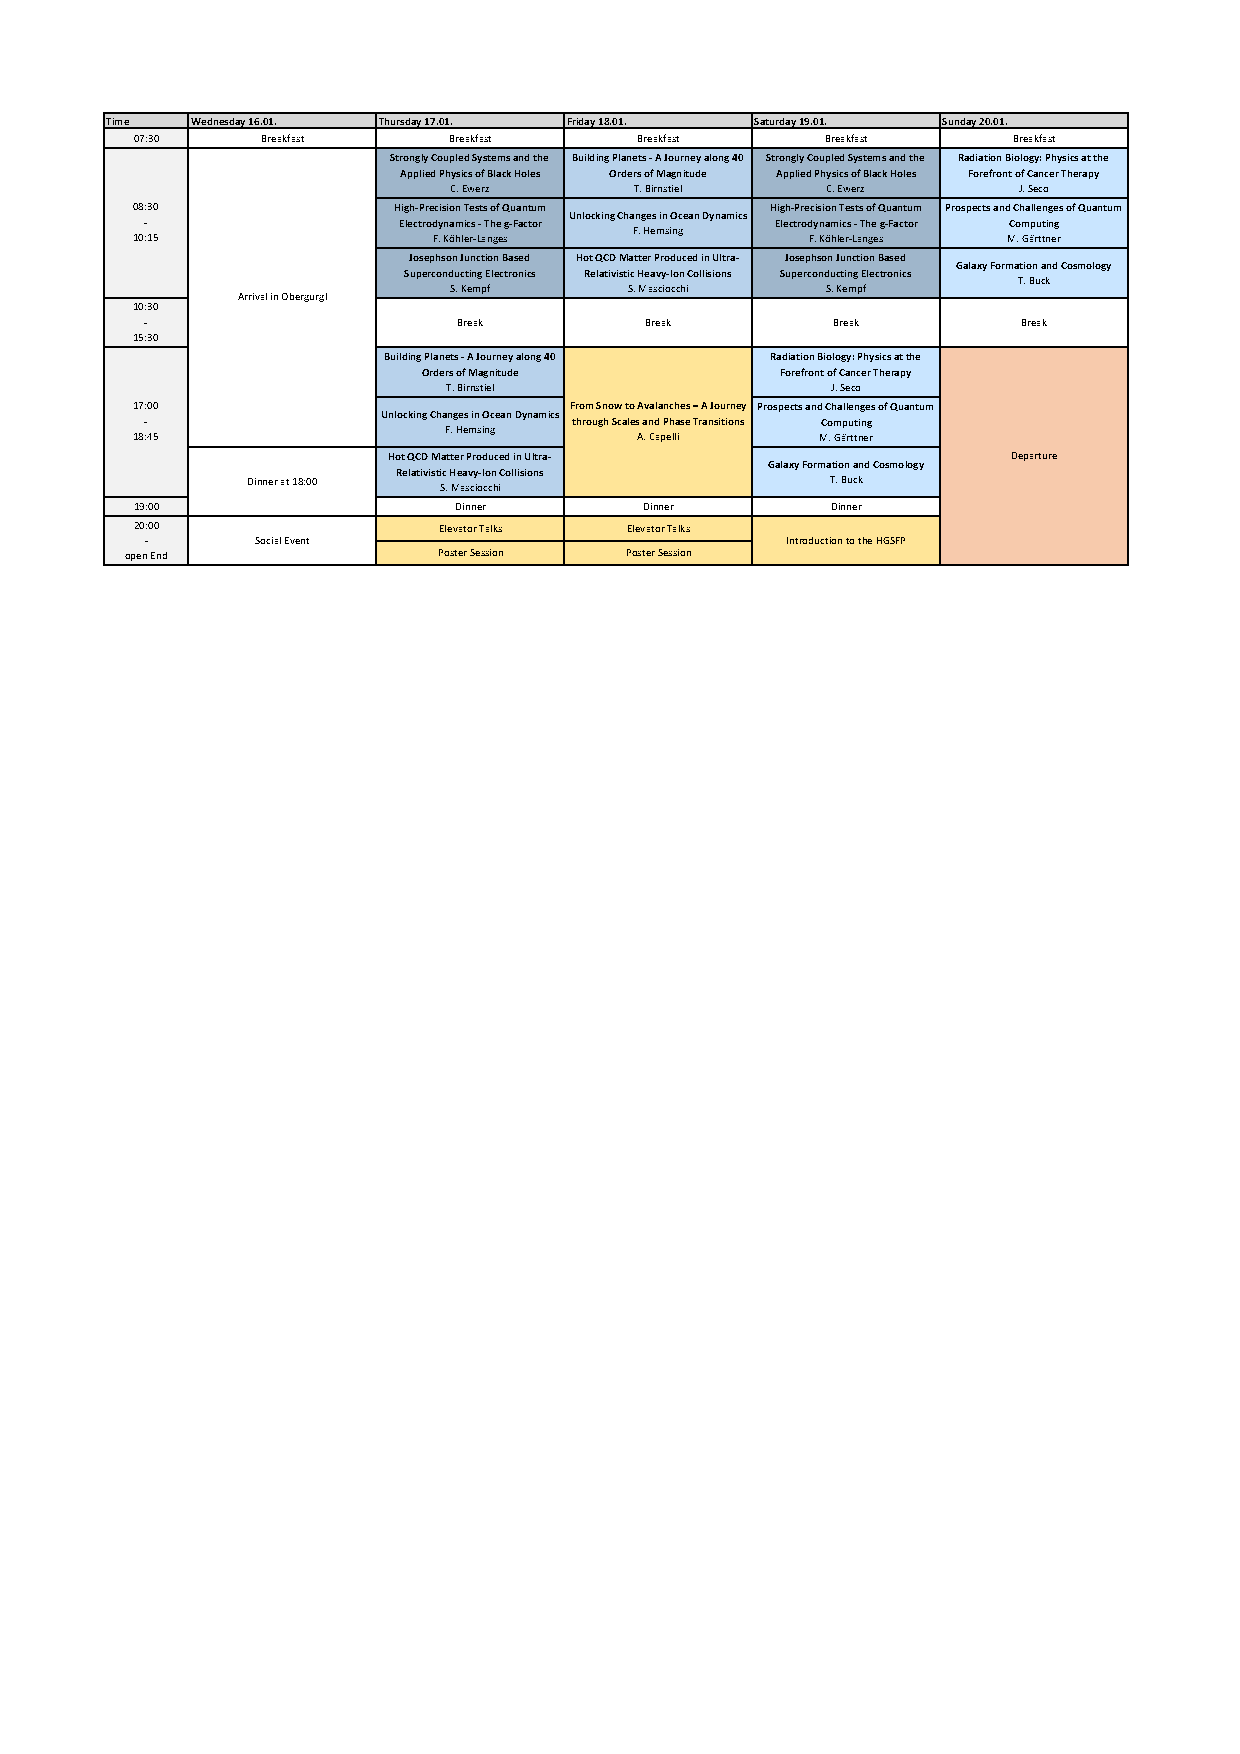
\includegraphics[scale=0.71, angle = 90 ]{figures/Program.pdf}
\end{figure}


\section*{B $\qquad$ Evaluation}

\subsection*{B1 $\qquad$ General Evaluation}
\pdfbookmark{B1 General Evaluation}{label:gevo}
\begin{figure}[h!]
  \centering
  \begin{minipage}{.48\linewidth}
    \centering
      {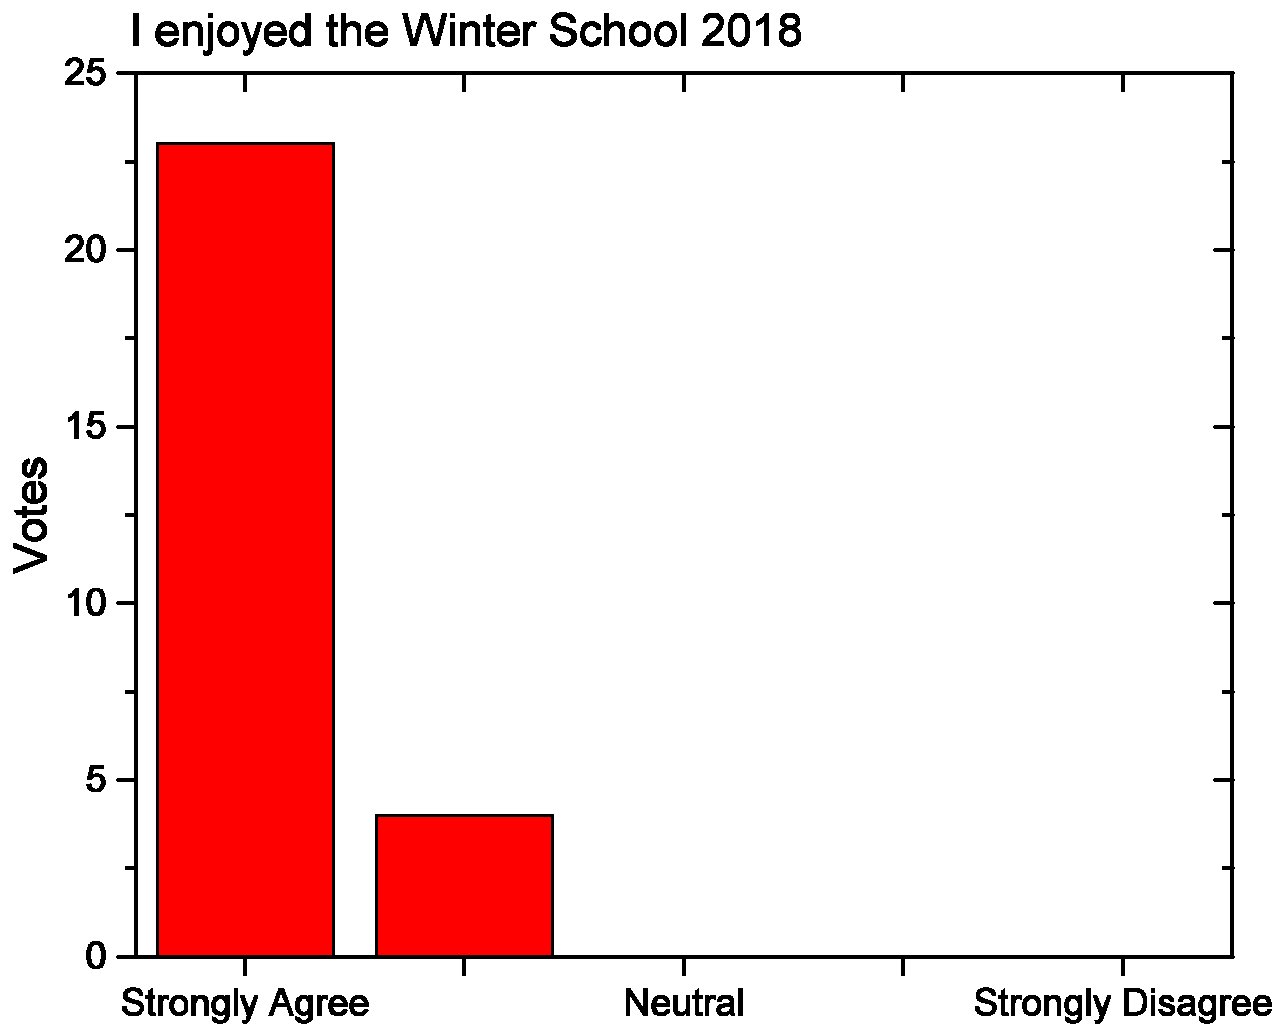
\includegraphics[height=50mm]{figures/n/Graph1.pdf}}
      {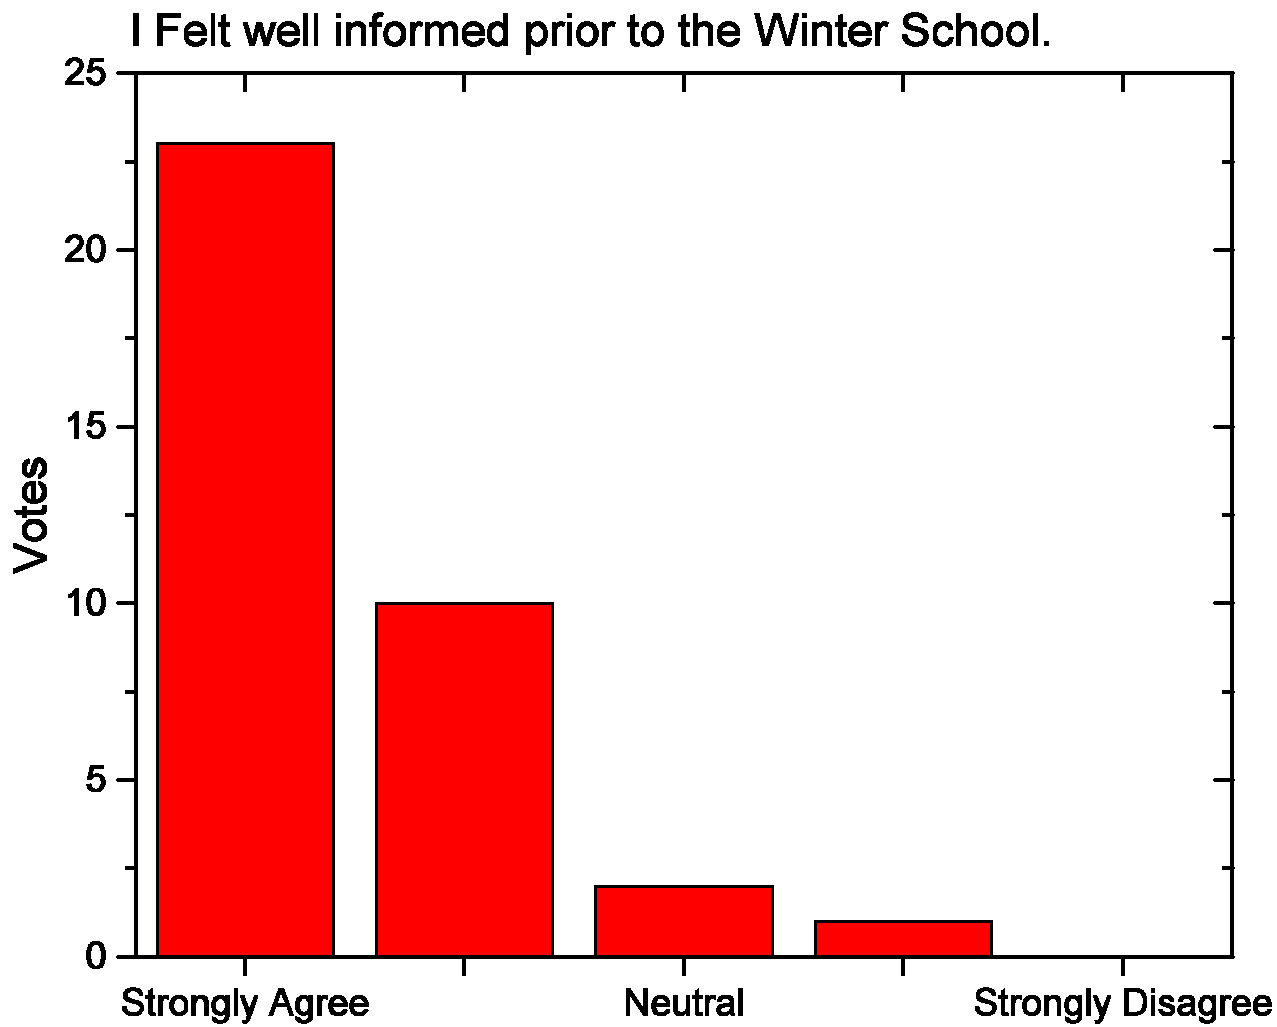
\includegraphics[height=50mm]{figures/n/Graph2.pdf}}
      {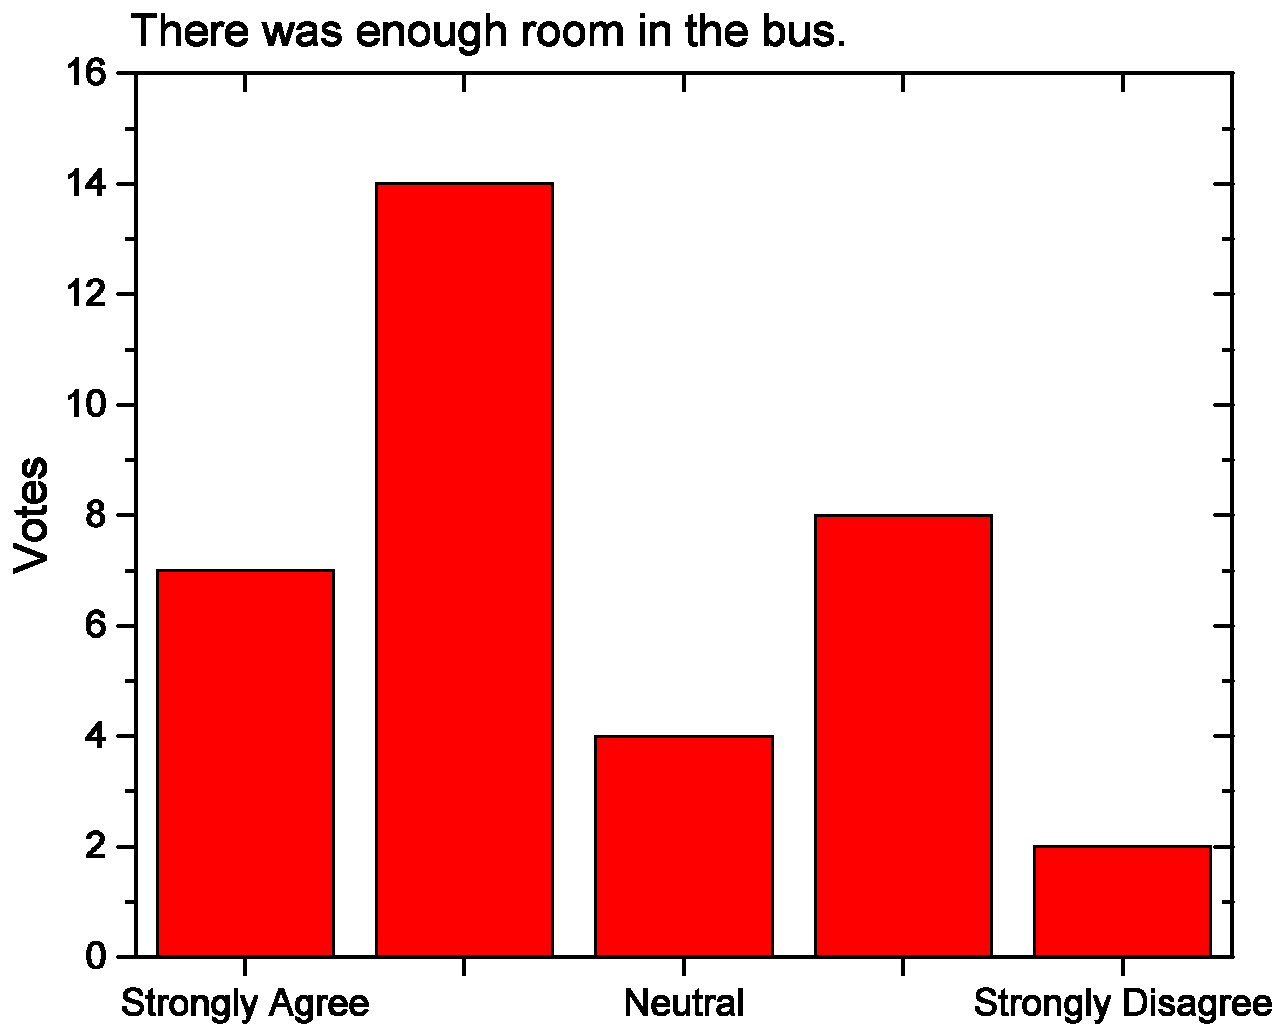
\includegraphics[height=50mm]{figures/n/Graph3.pdf}}
  \end{minipage}\quad
  \begin{minipage}{.48\linewidth}
    \centering
      {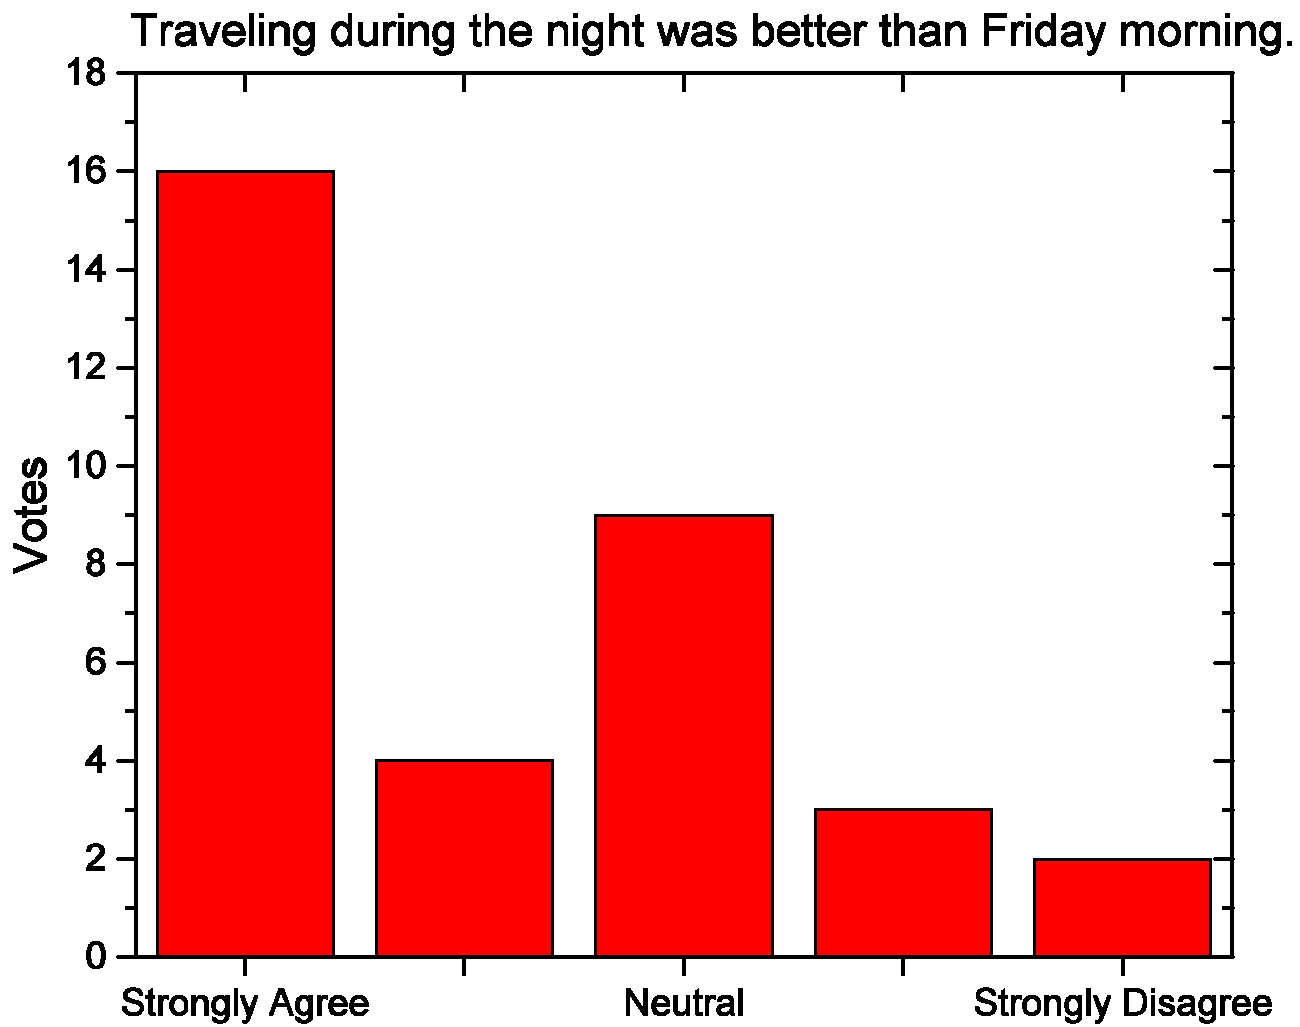
\includegraphics[height=50mm]{figures/n/Graph4.pdf}}
      {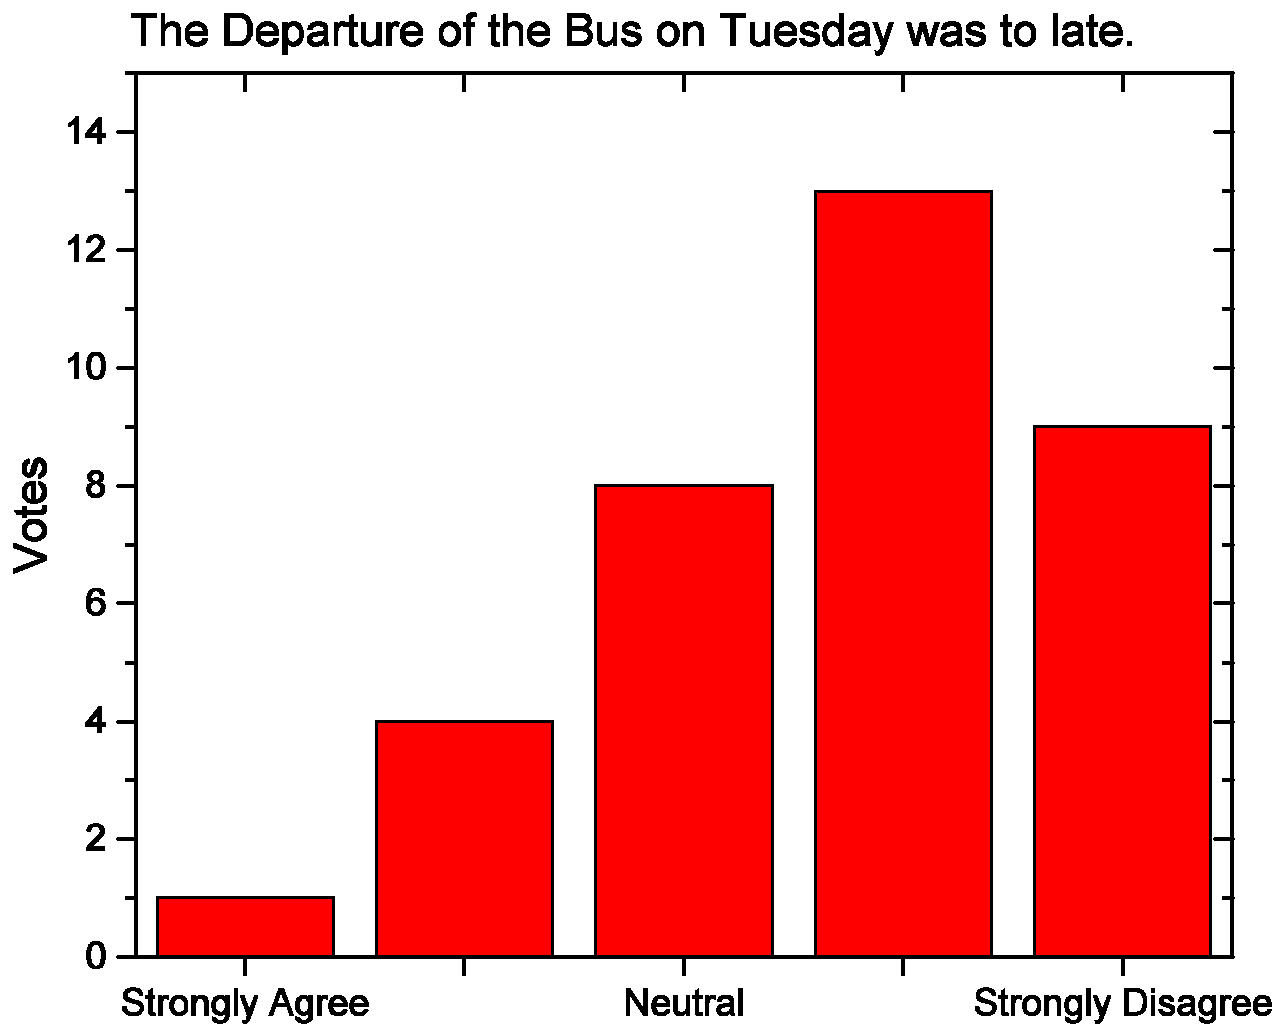
\includegraphics[height=50mm]{figures/n/Graph5.pdf}}
      {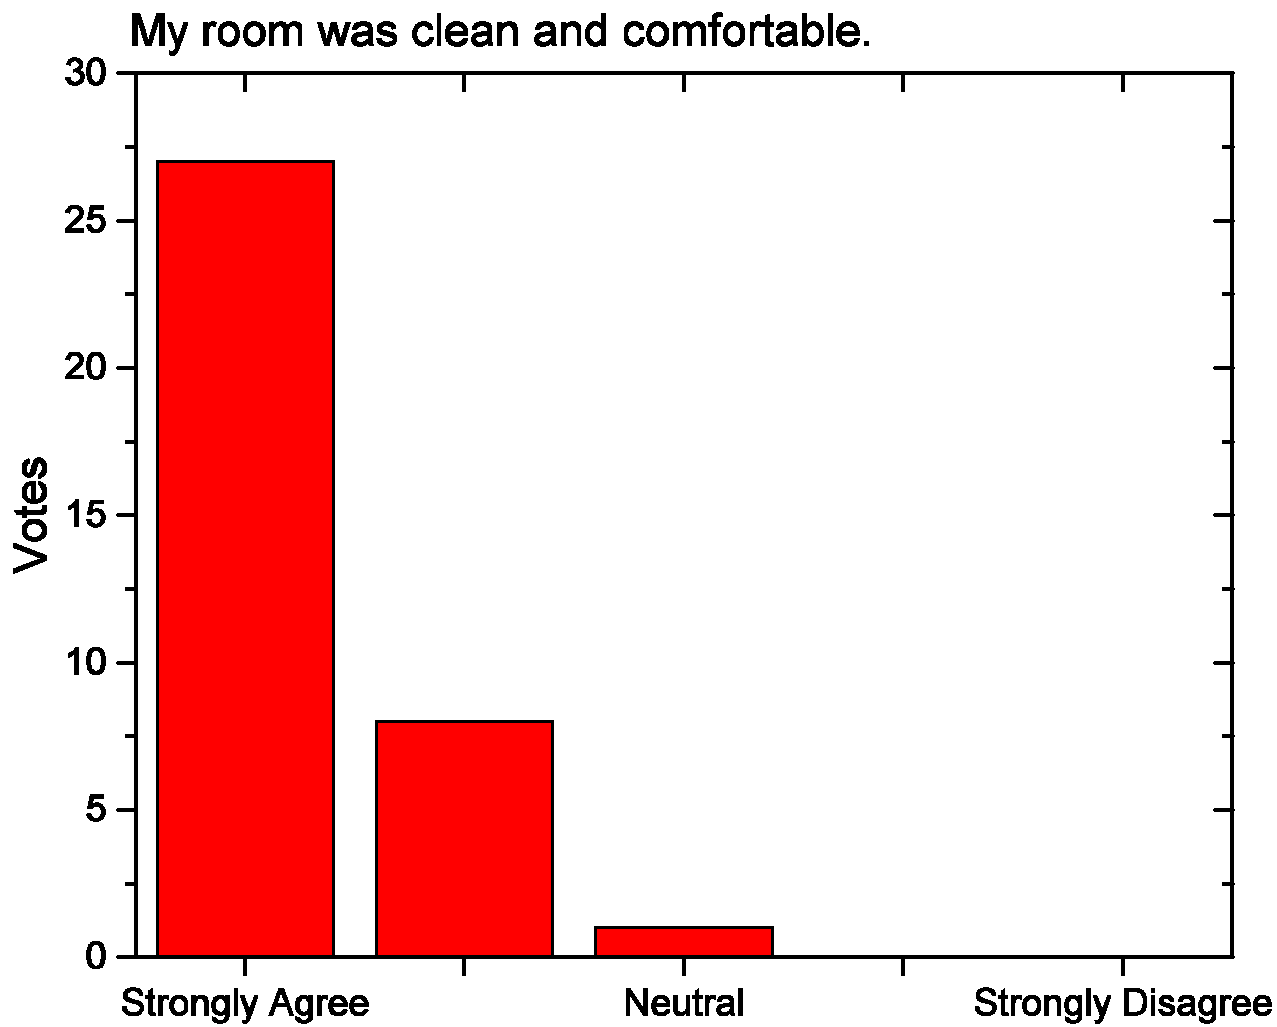
\includegraphics[height=50mm]{figures/n/Graph6.pdf}}
  \end{minipage}
\end{figure}

\begin{figure}[H]
  \centering
  \begin{minipage}{.48\linewidth}
    \centering
      {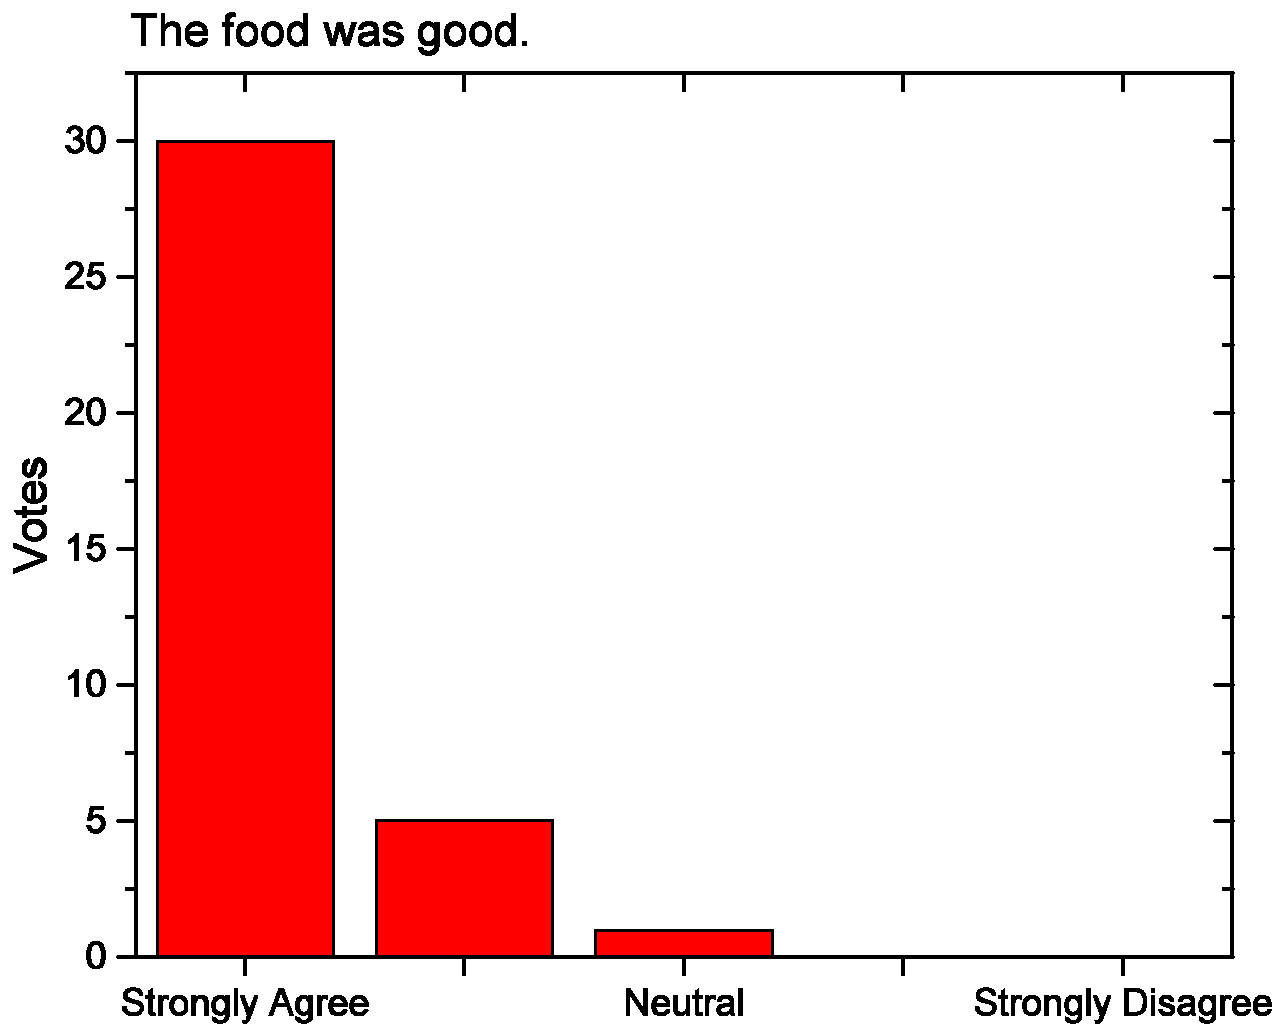
\includegraphics[height=50mm]{figures/n/Graph7.pdf}}
      {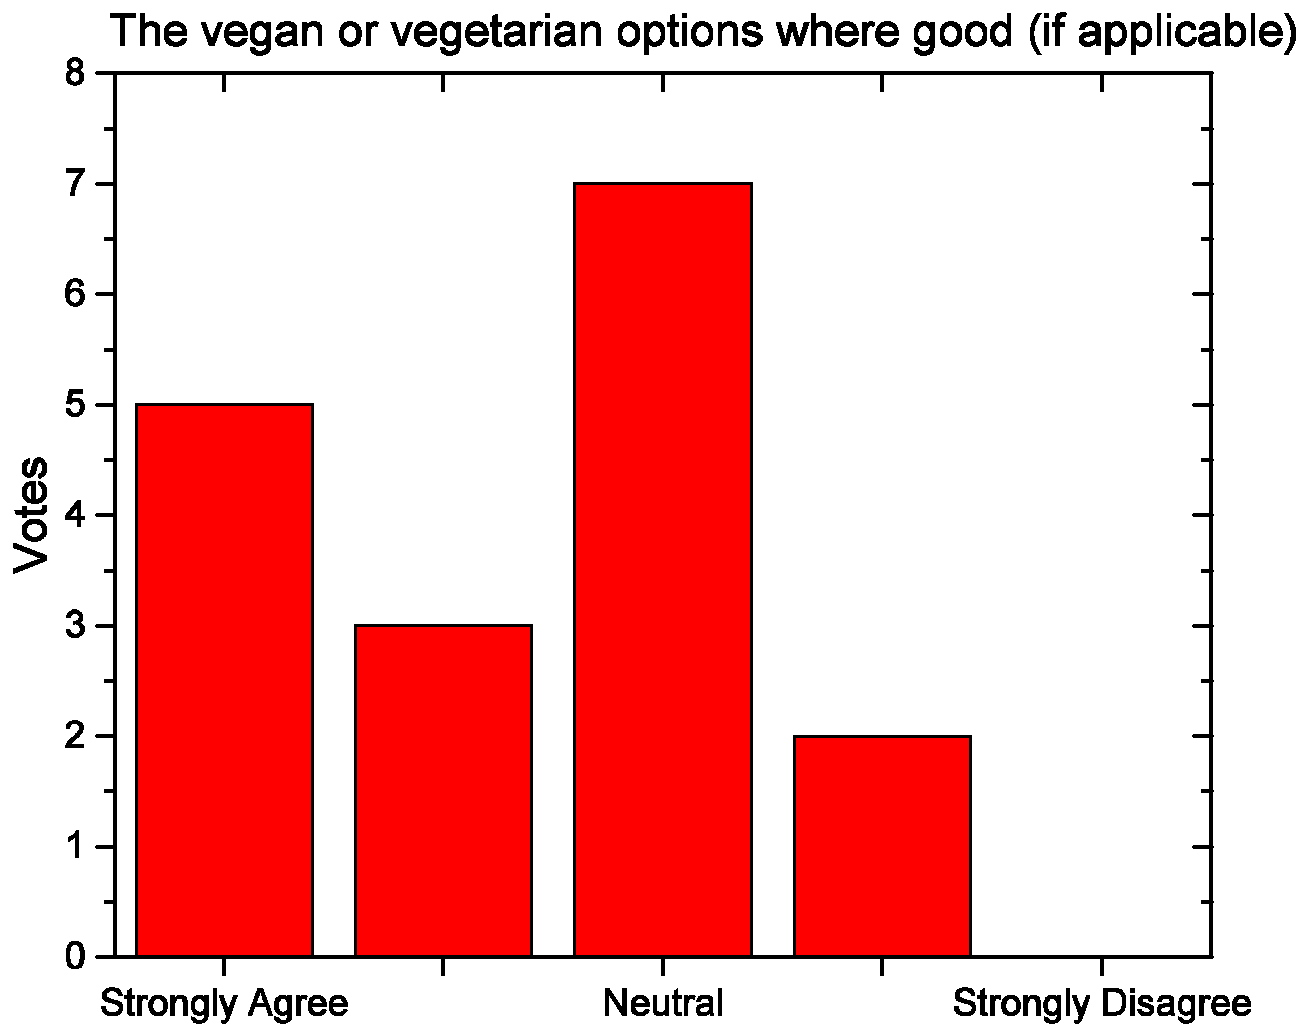
\includegraphics[height=50mm]{figures/n/Graph8.pdf}}
      {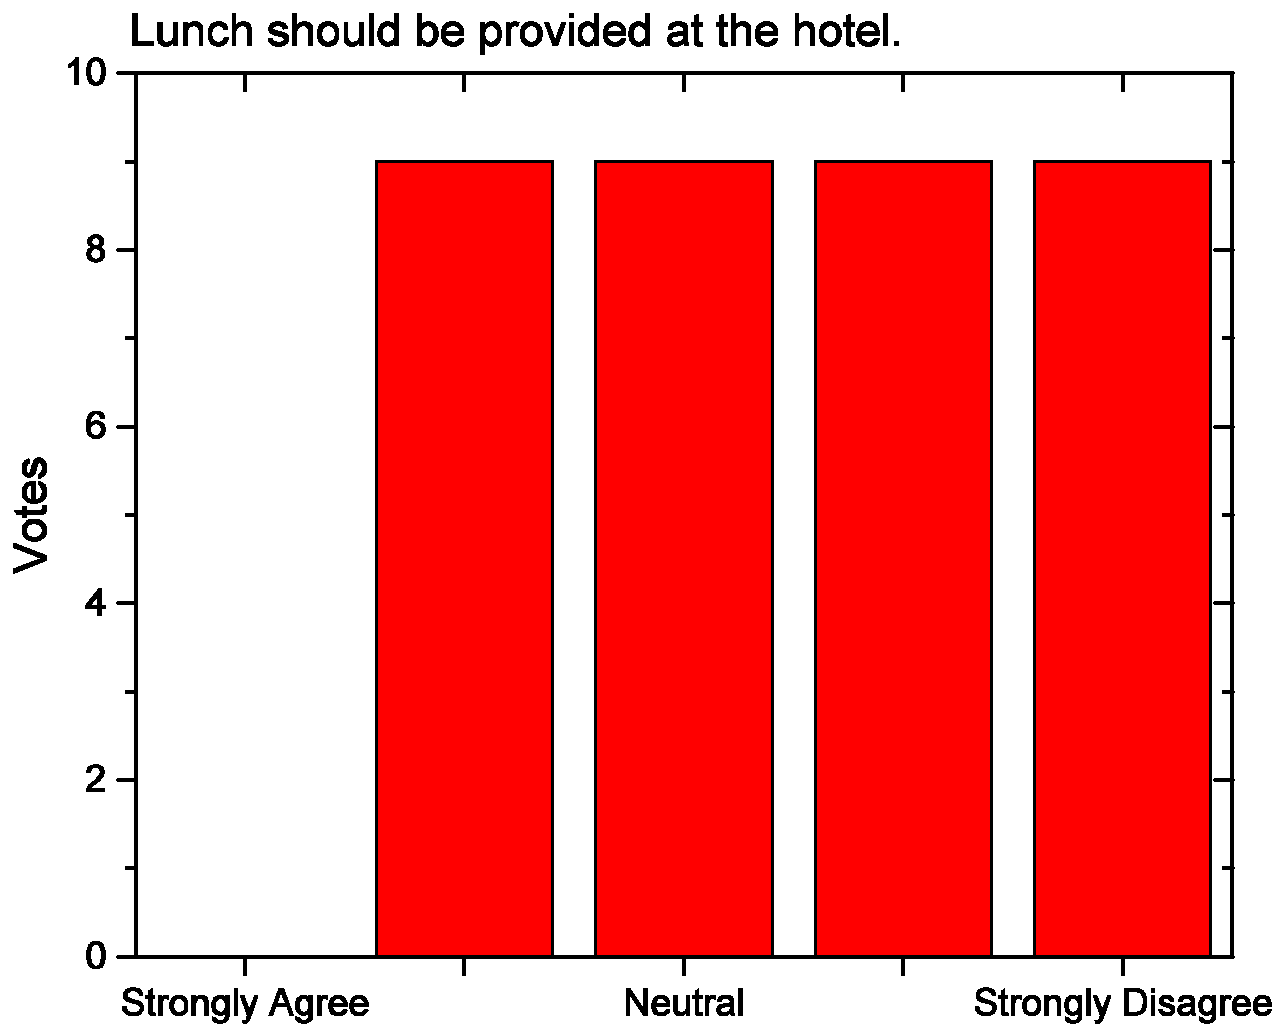
\includegraphics[height=50mm]{figures/n/Graph9.pdf}}
      {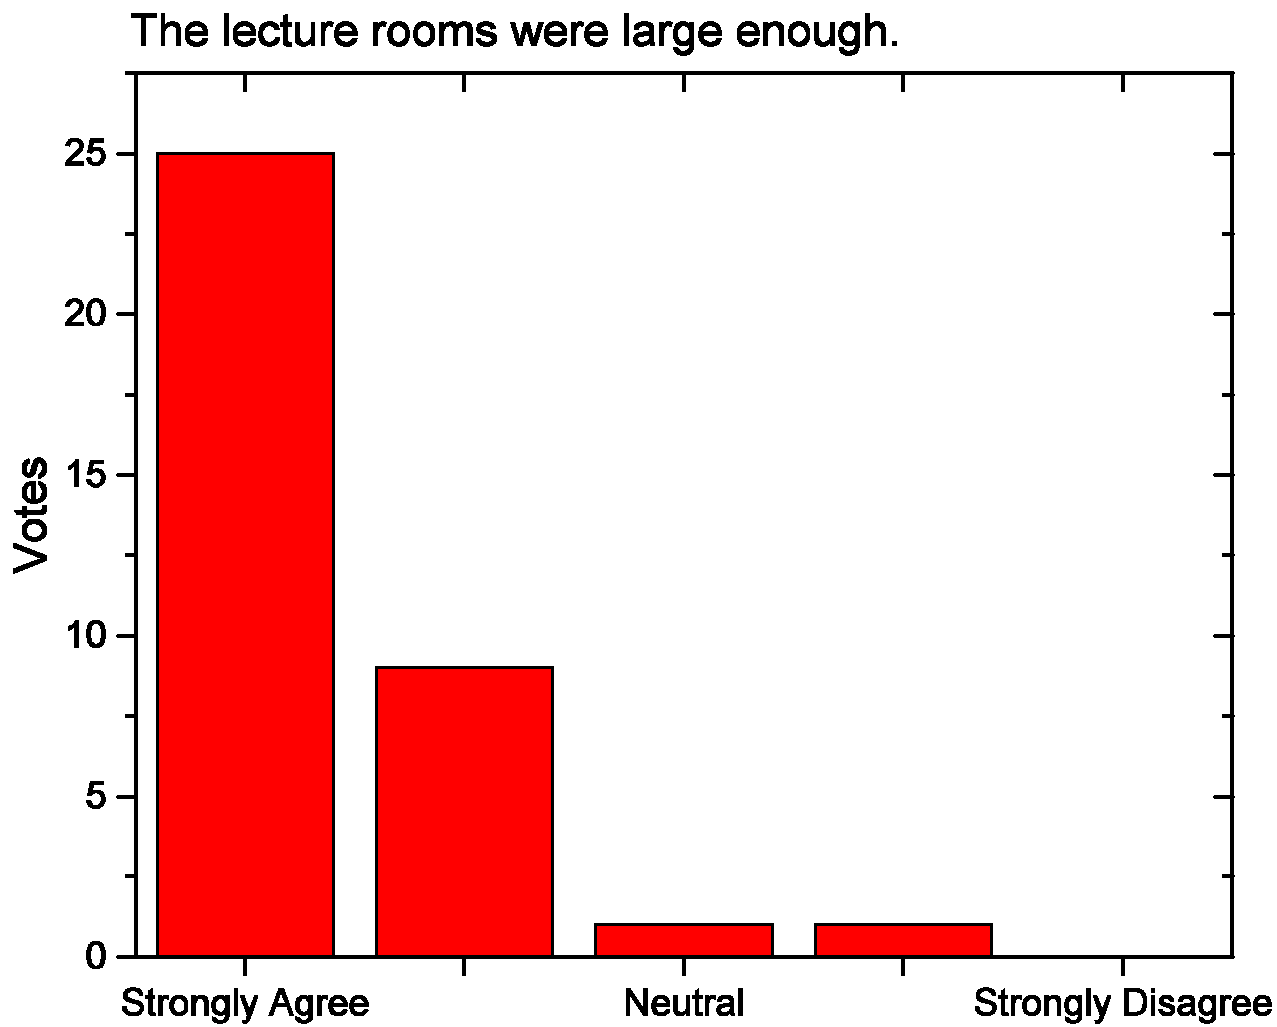
\includegraphics[height=50mm]{figures/n/Graph10.pdf}}
  \end{minipage}\quad
  \begin{minipage}{.48\linewidth}
    \centering
      {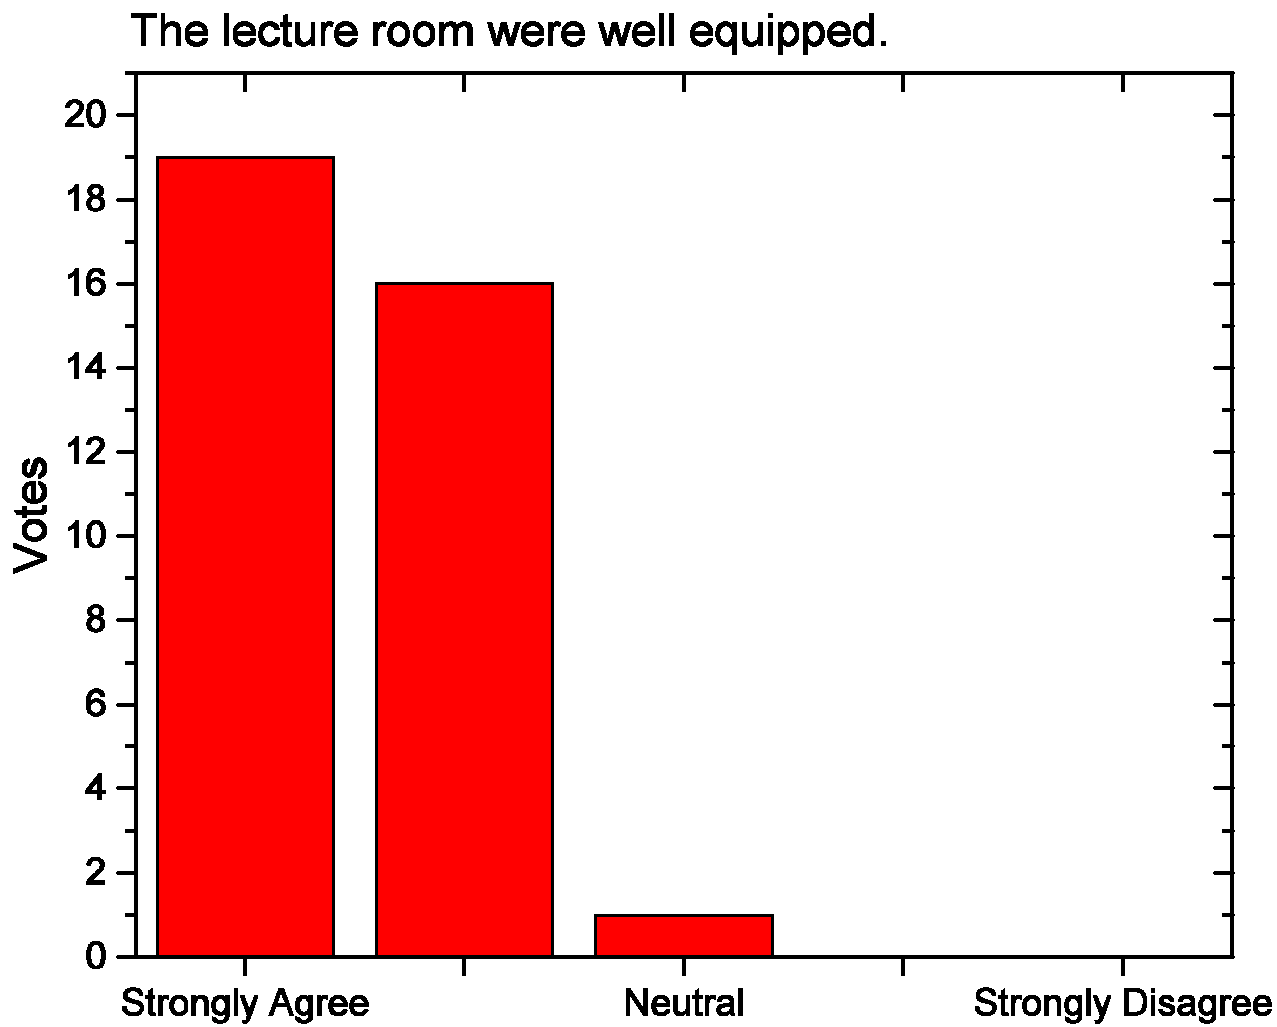
\includegraphics[height=50mm]{figures/n/Graph11.pdf}}
      {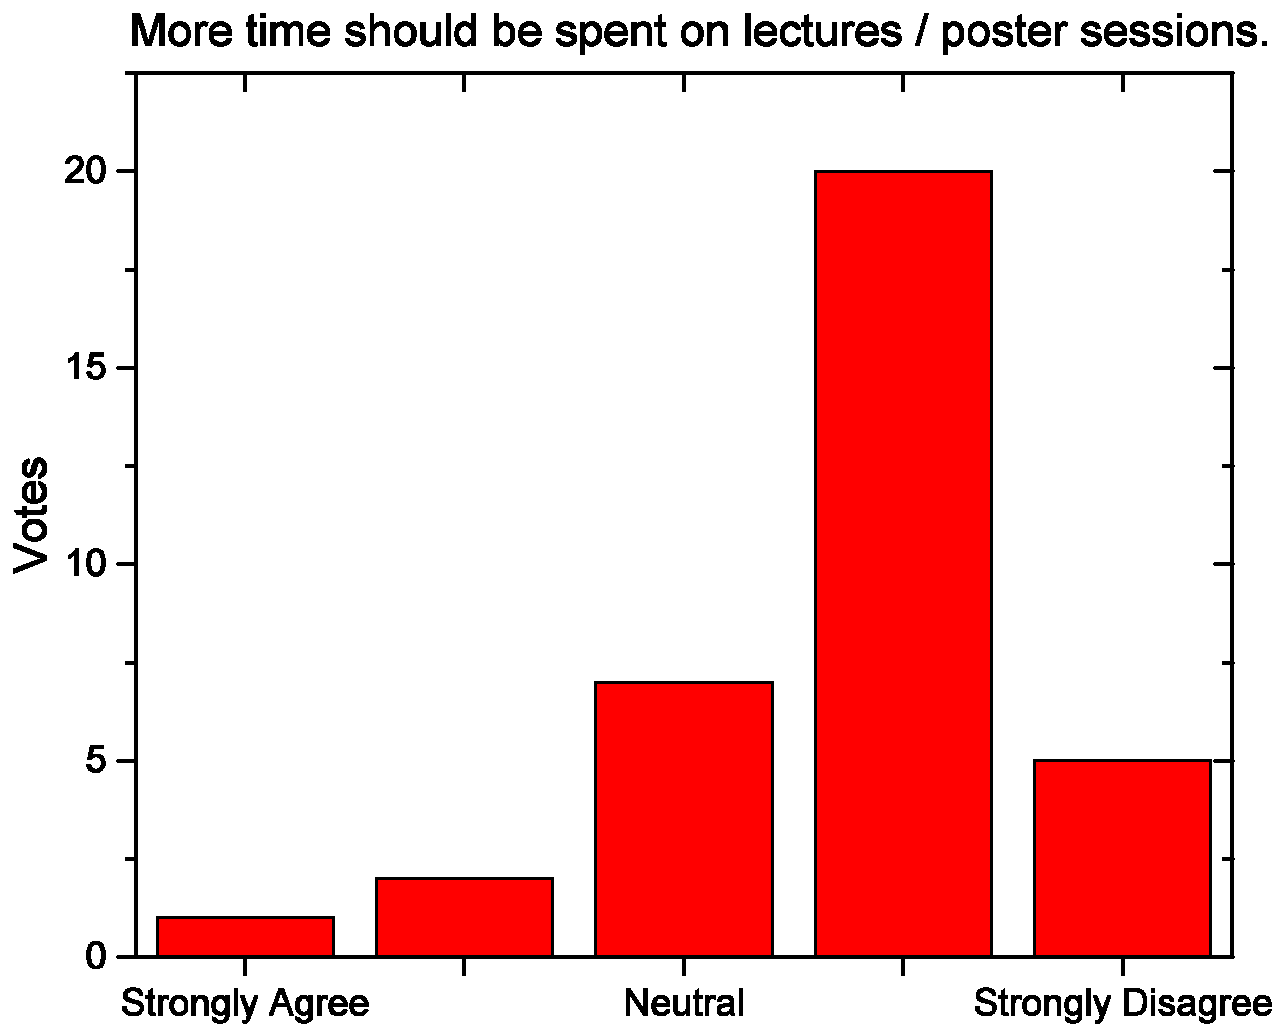
\includegraphics[height=50mm]{figures/n/Graph12.pdf}}
      {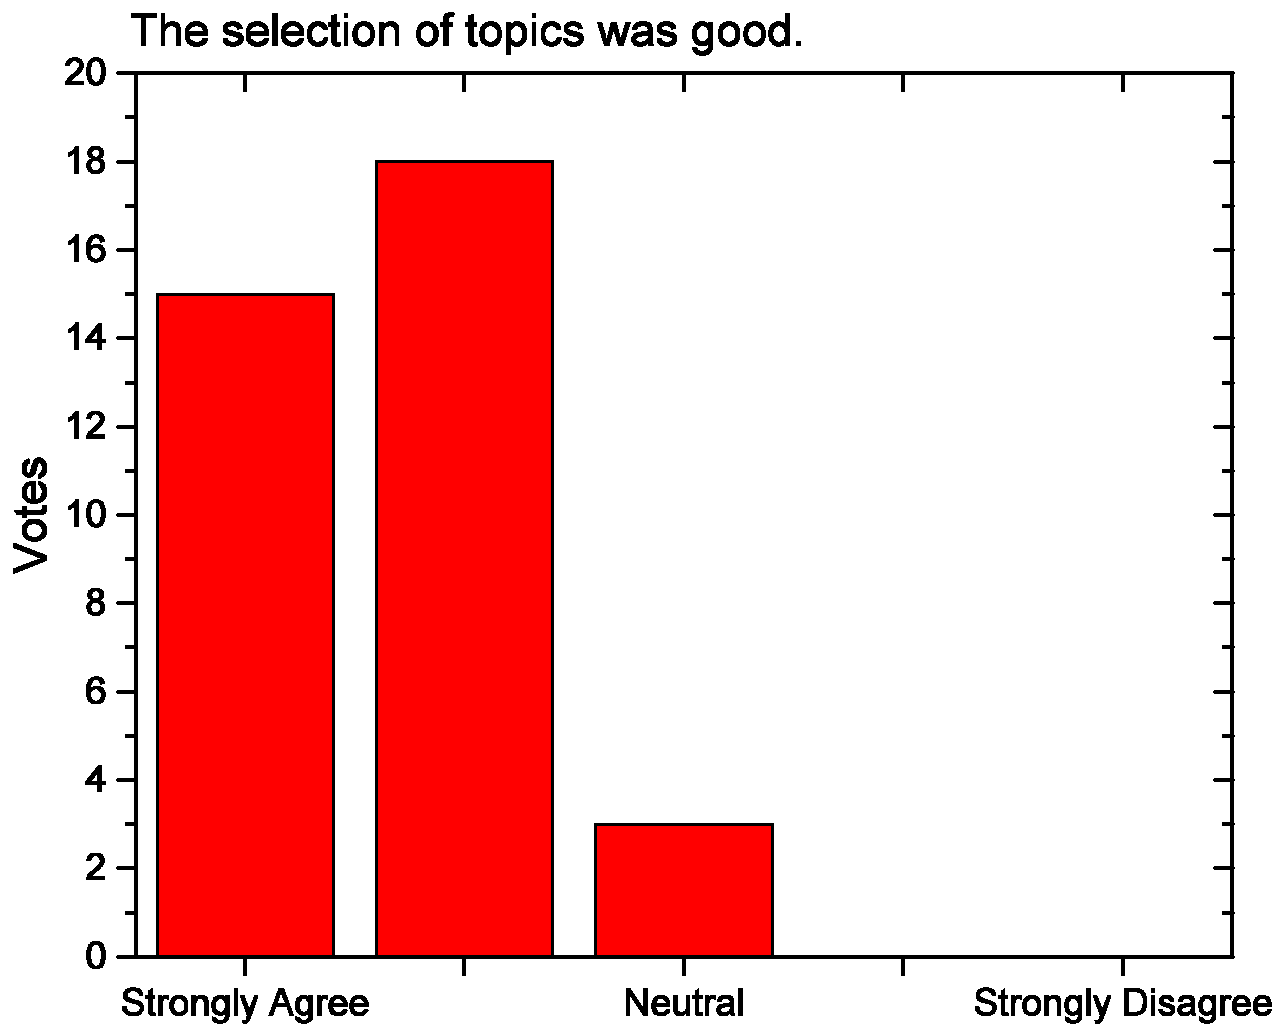
\includegraphics[height=50mm]{figures/n/Graph13.pdf}}
      {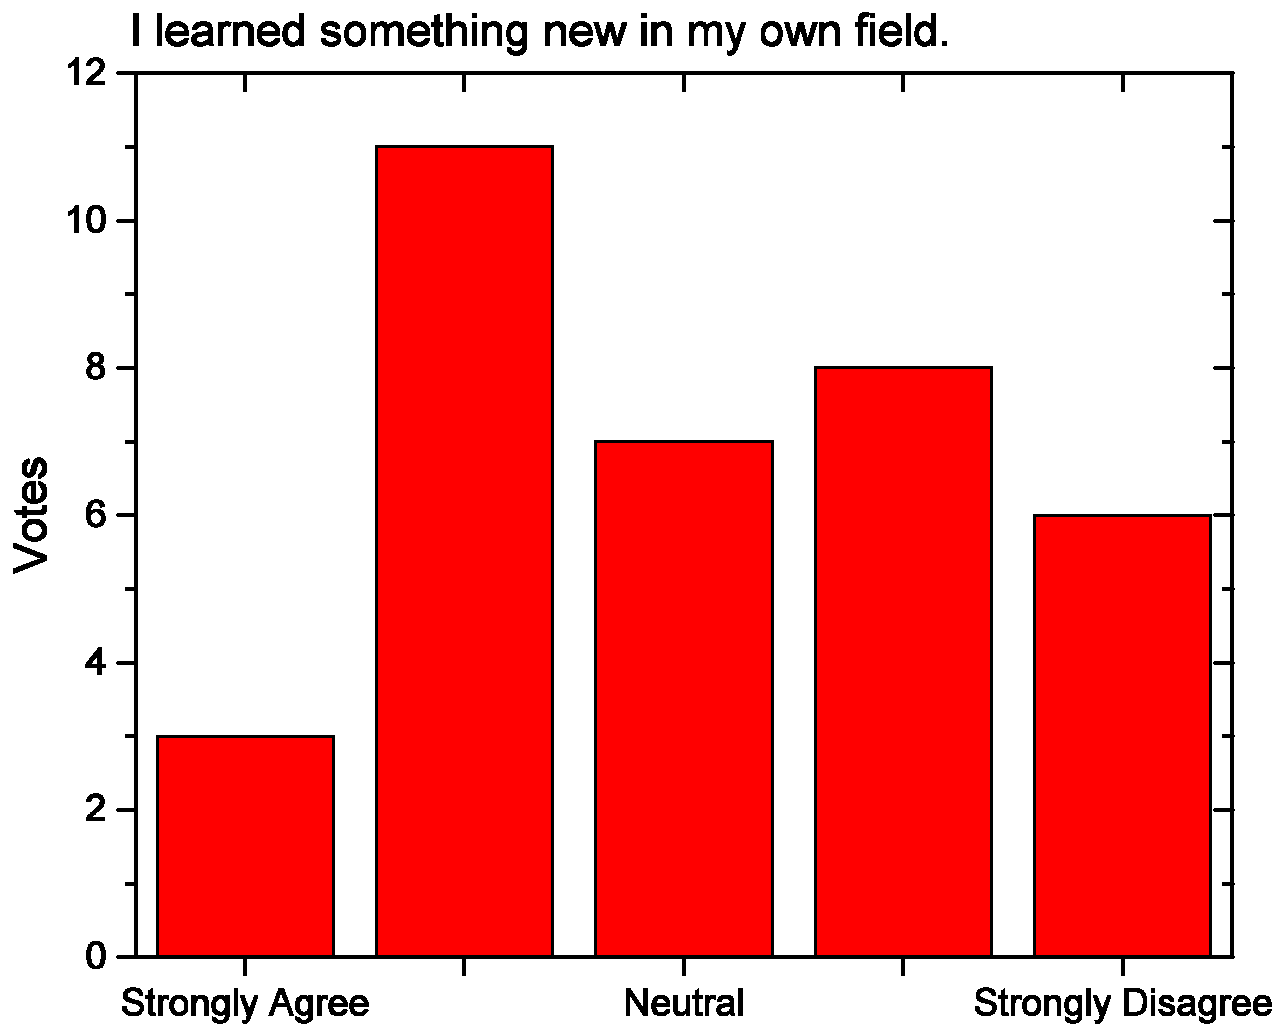
\includegraphics[height=50mm]{figures/n/Graph14.pdf}}
  \end{minipage}
\end{figure}

\begin{figure}[H]
  \centering
  \begin{minipage}{.48\linewidth}
    \centering
      {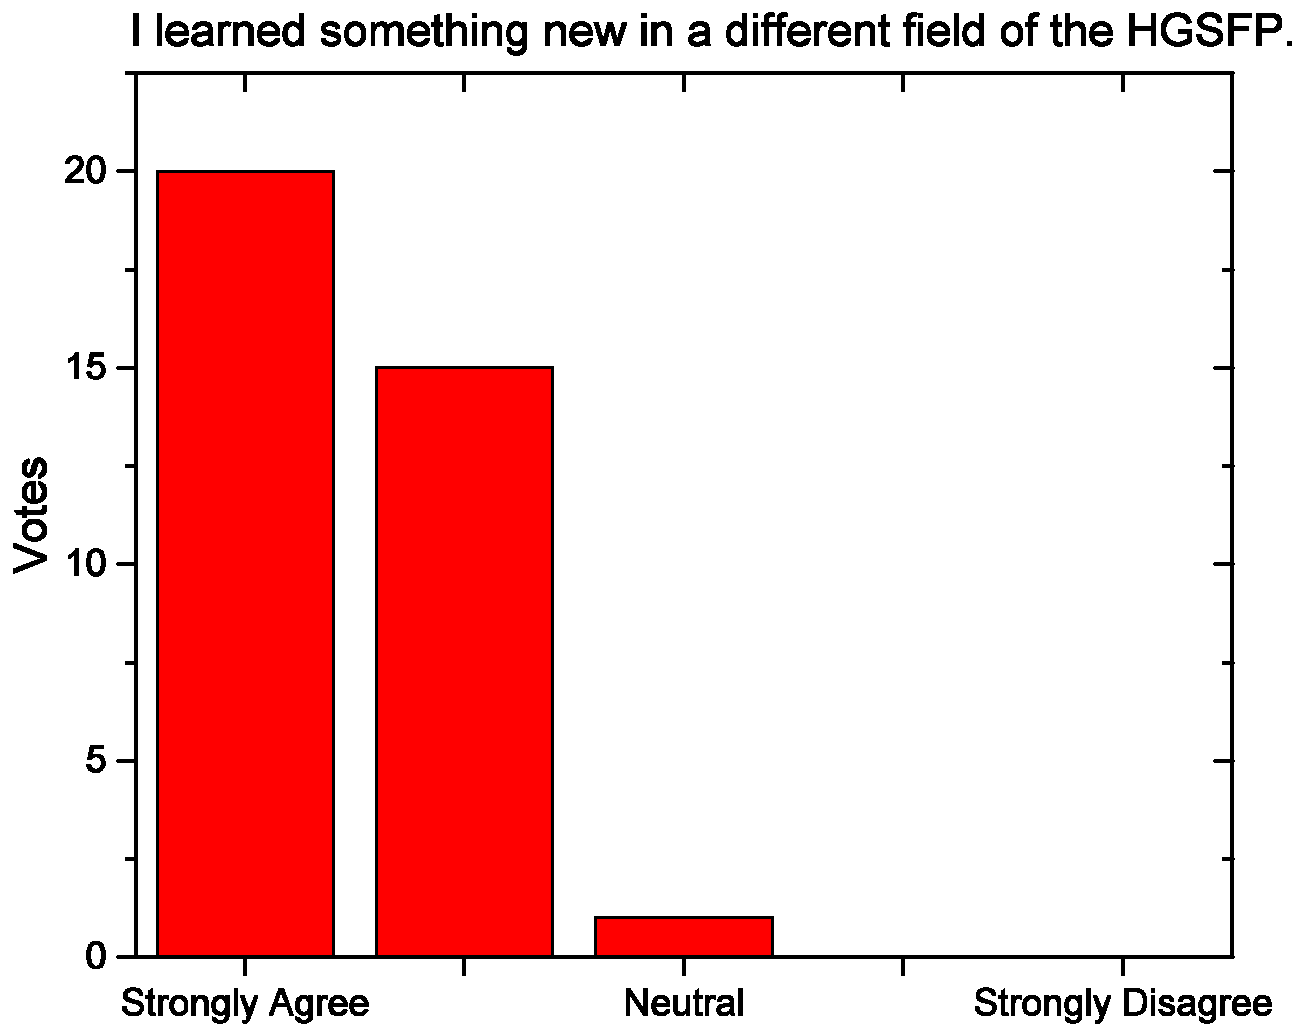
\includegraphics[height=50mm]{figures/n/Graph15.pdf}}
      {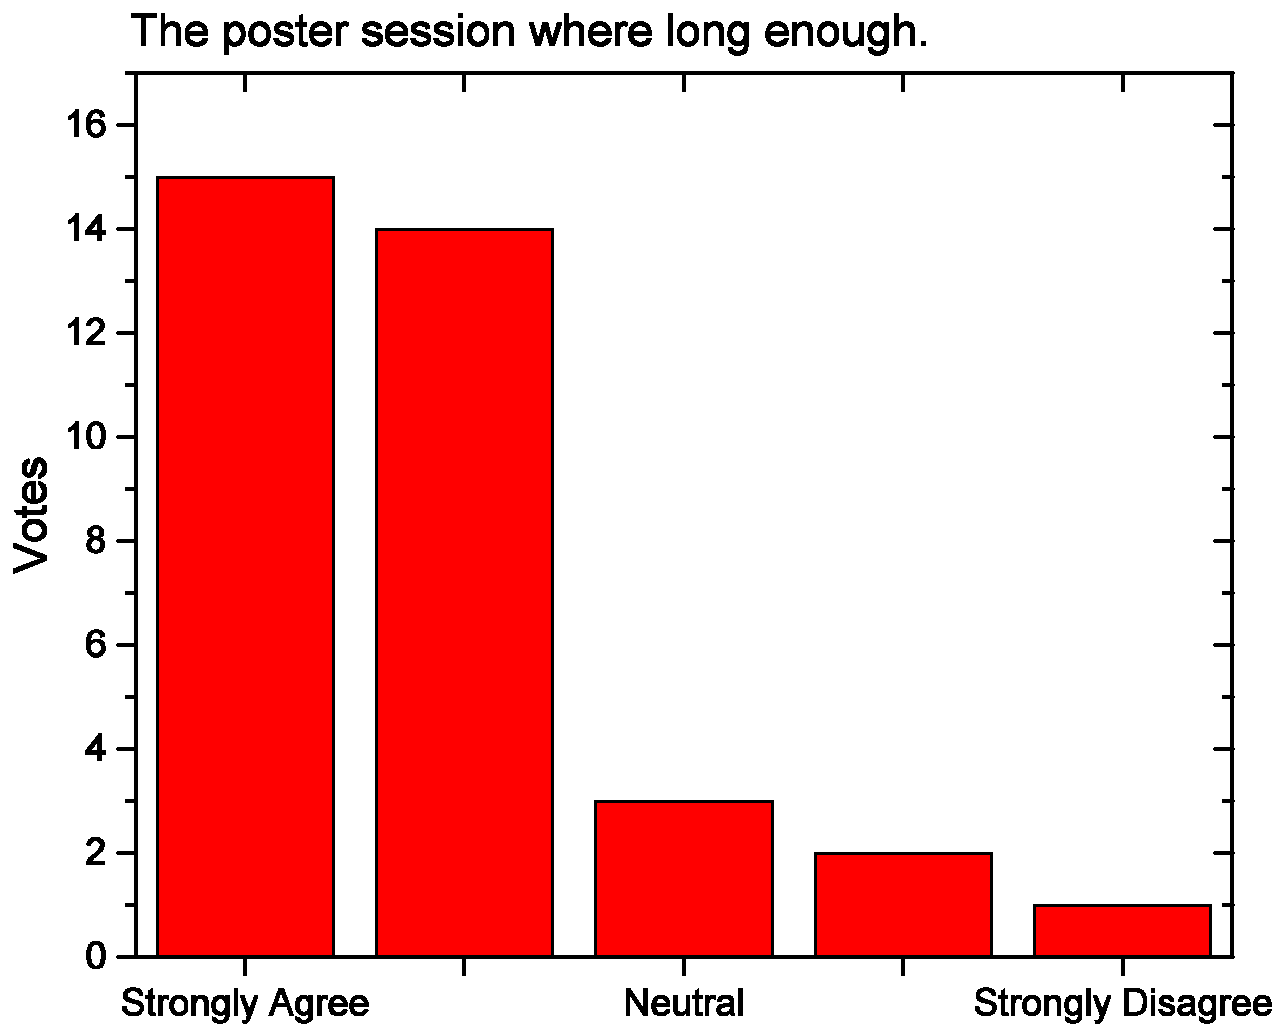
\includegraphics[height=50mm]{figures/n/Graph16.pdf}}
      {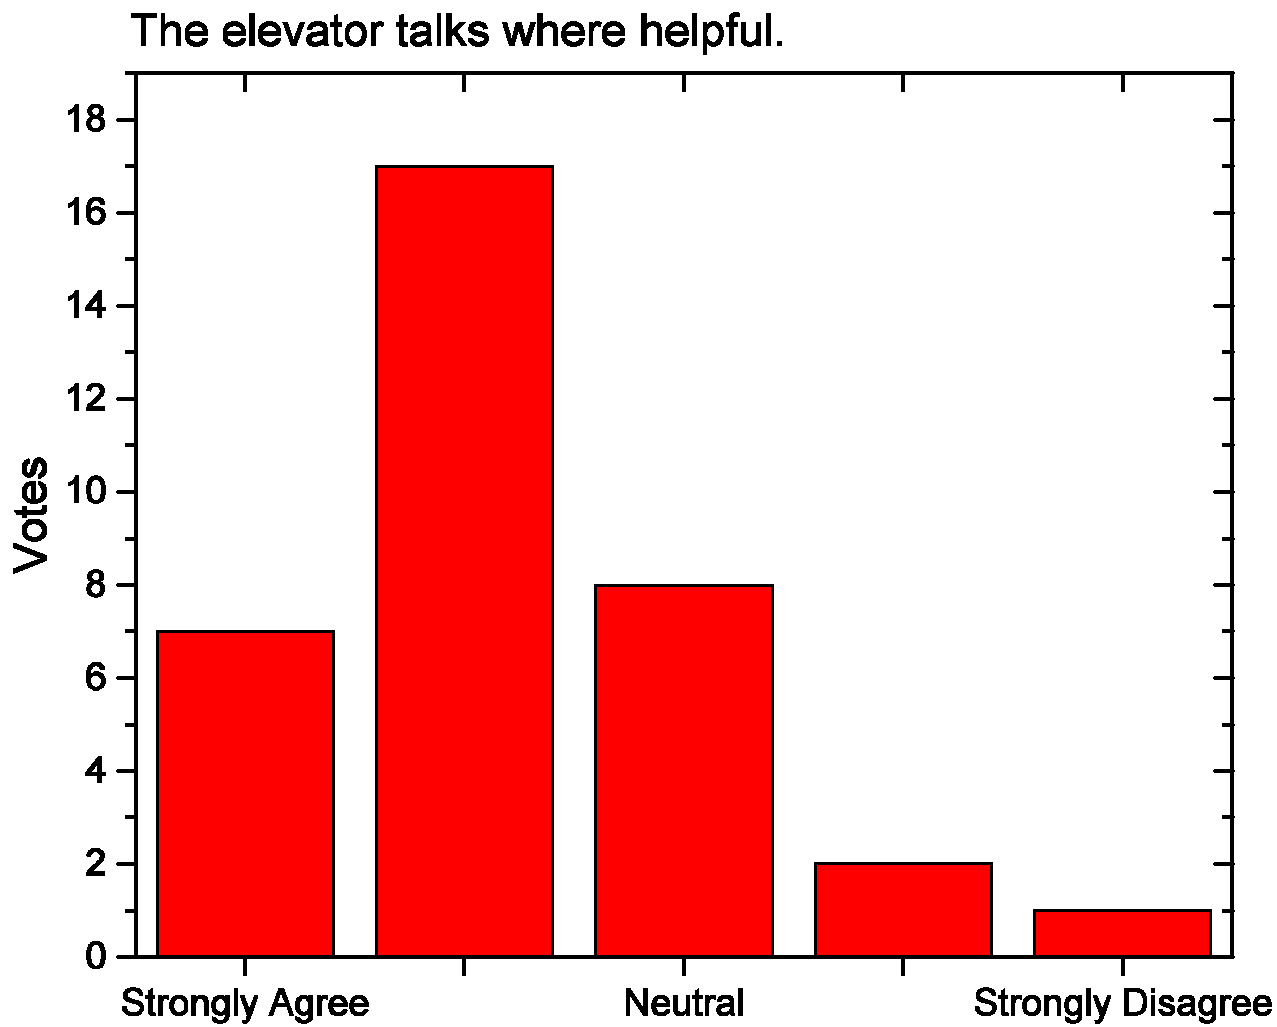
\includegraphics[height=50mm]{figures/n/Graph17.pdf}}
  \end{minipage}\quad
  \begin{minipage}{.48\linewidth}
    \centering
      {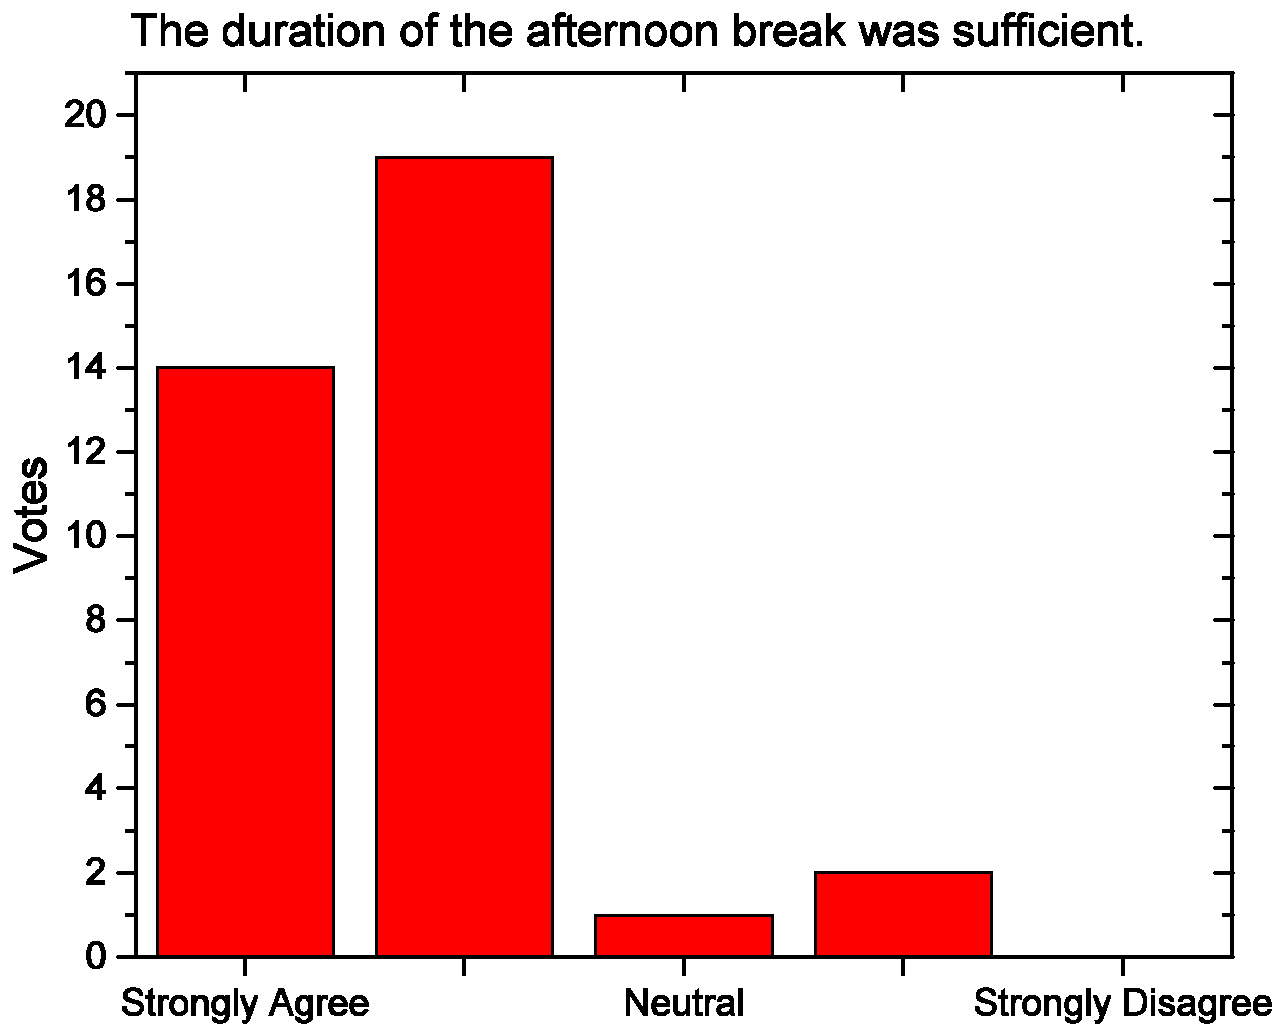
\includegraphics[height=50mm]{figures/n/Graph18.pdf}}
      {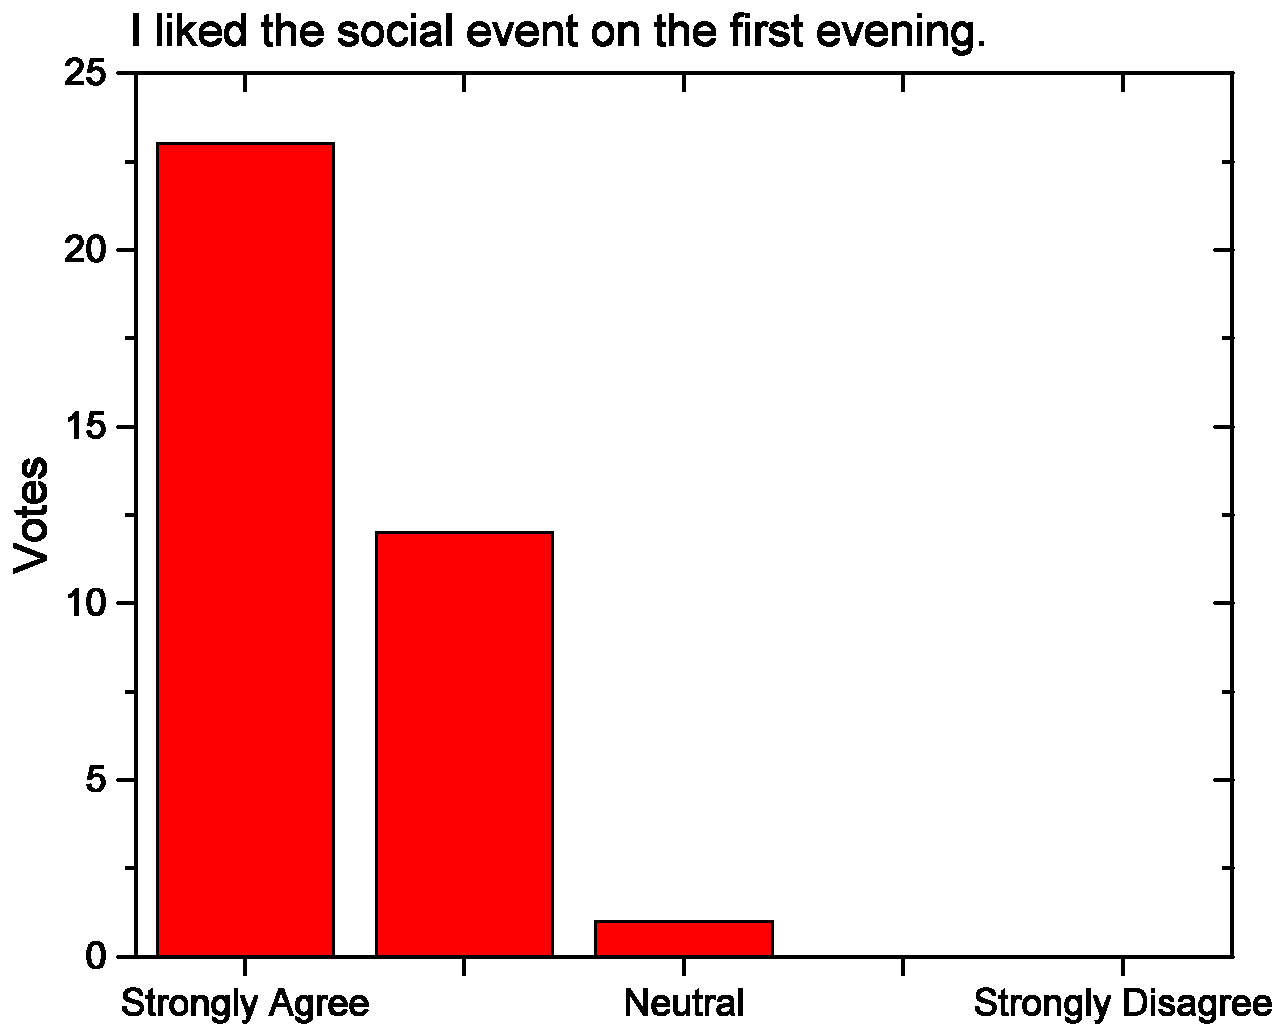
\includegraphics[height=50mm]{figures/n/Graph19.pdf}}
      {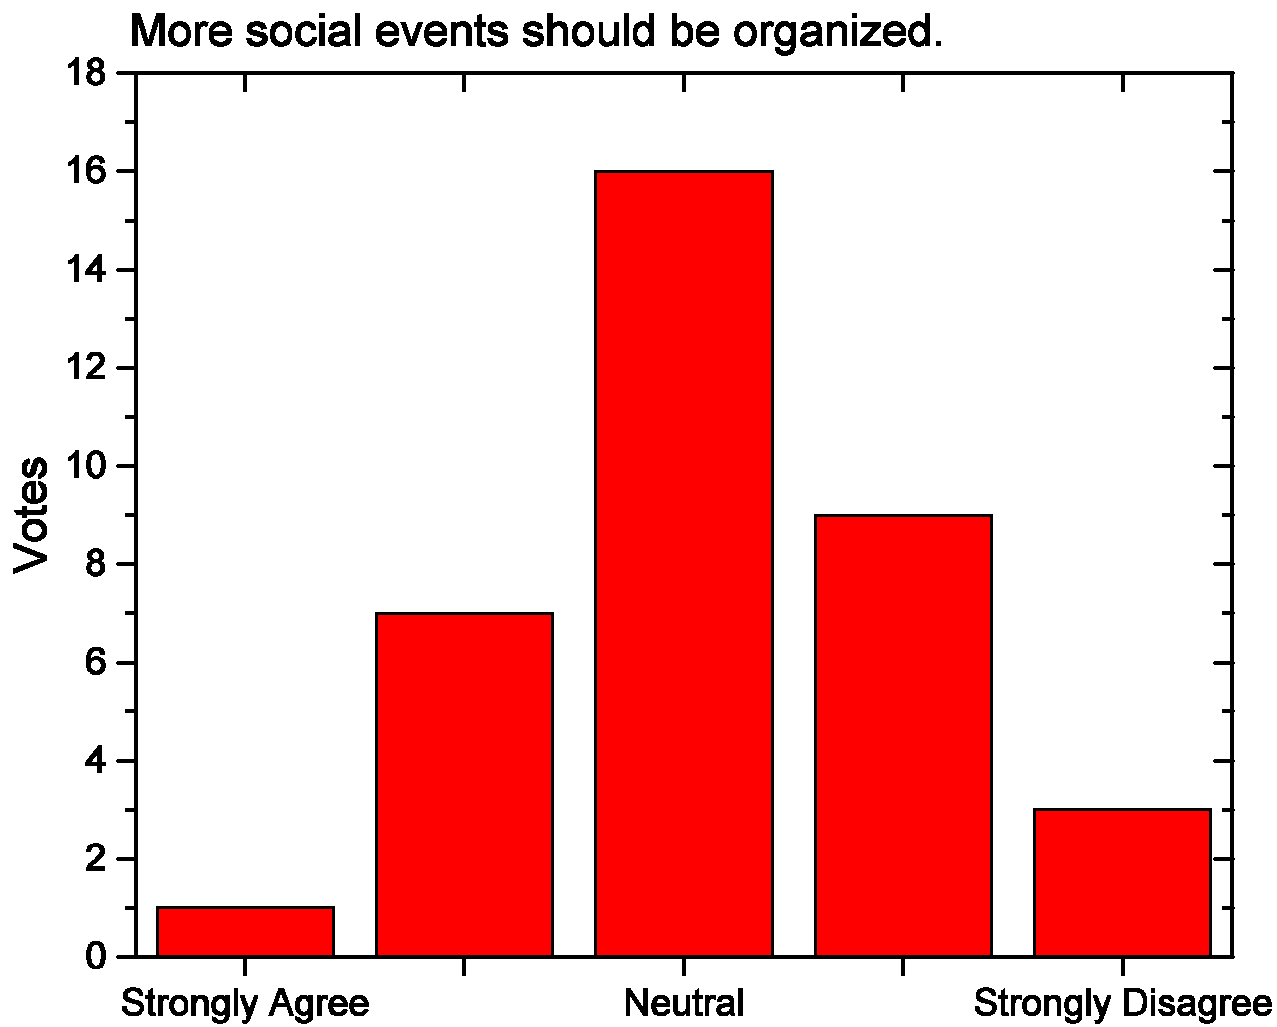
\includegraphics[height=50mm]{figures/n/Graph20.pdf}}
  \end{minipage}
\end{figure}
\subsubsection*{Comments}
\begin{itemize}
\item Great Hotel
\item Reduce the amount of parallel sessions.
\item More time for breakfast by starting lectures at 9.
\item Telegram group was a nice idea.
\item Do HGSFP introduction lecture on first day.
\item Second social event on the last day would be great.
\end{itemize}

\clearpage
\subsection*{B2 $\qquad$ Lecture Evaluations}

\subsubsection{Philipp Prei{\ss}  --- Quantum Simulation with Ultracold Atoms }
\pdfbookmark{B2 Philipp Prei{\ss}}{label:pp}
\begin{figure}[h!]
  \centering
  \begin{minipage}{.48\linewidth}
    \centering
      {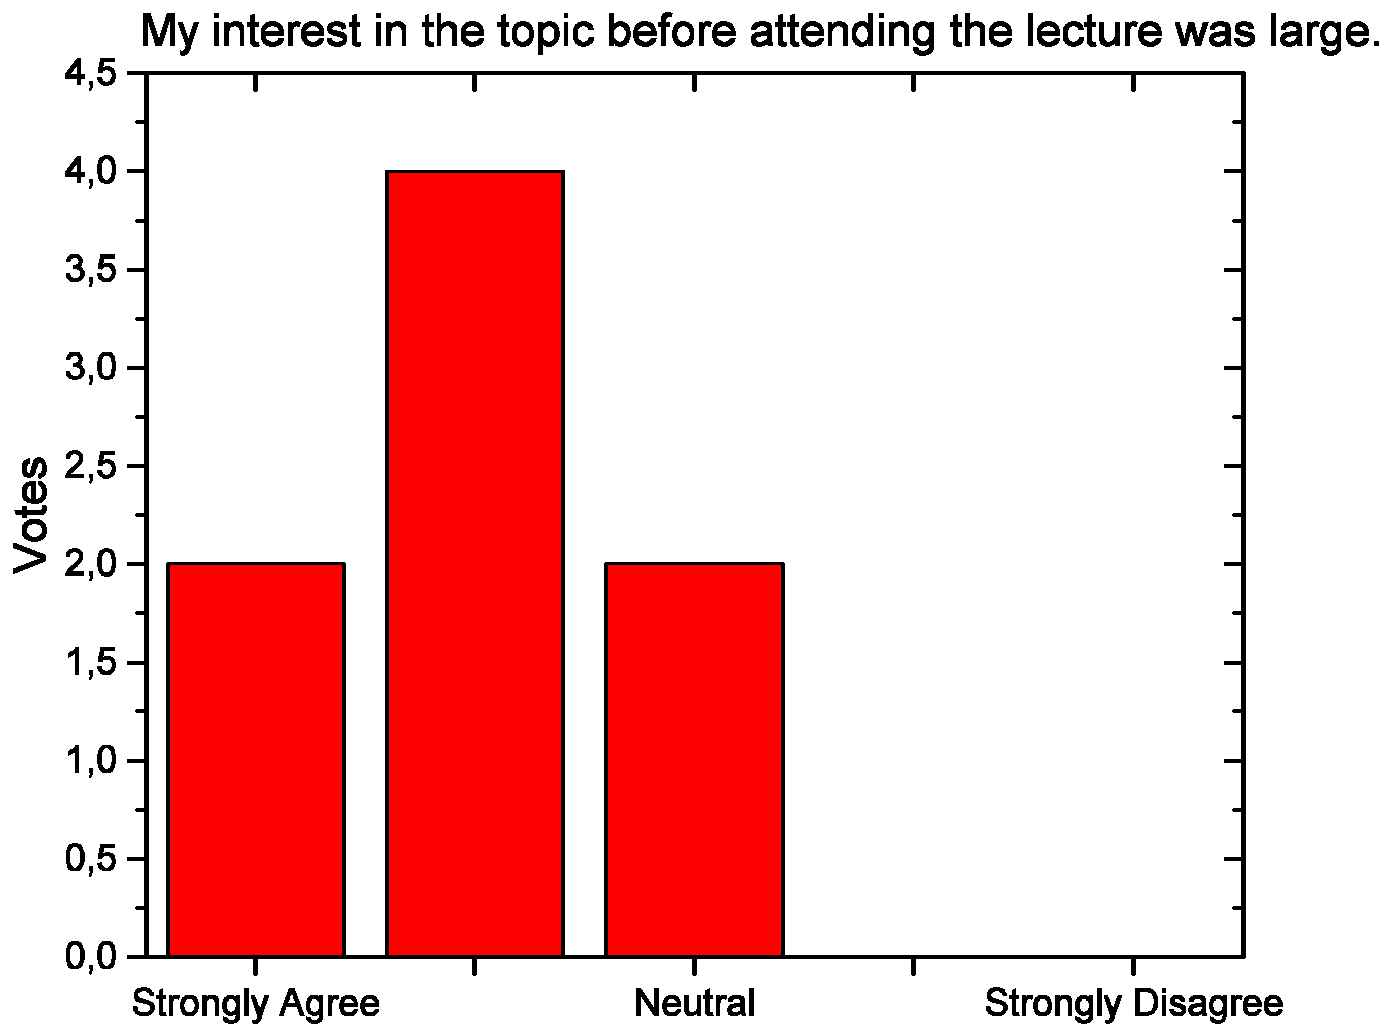
\includegraphics[height=50mm]{figures/n/Graph21.pdf}}
      {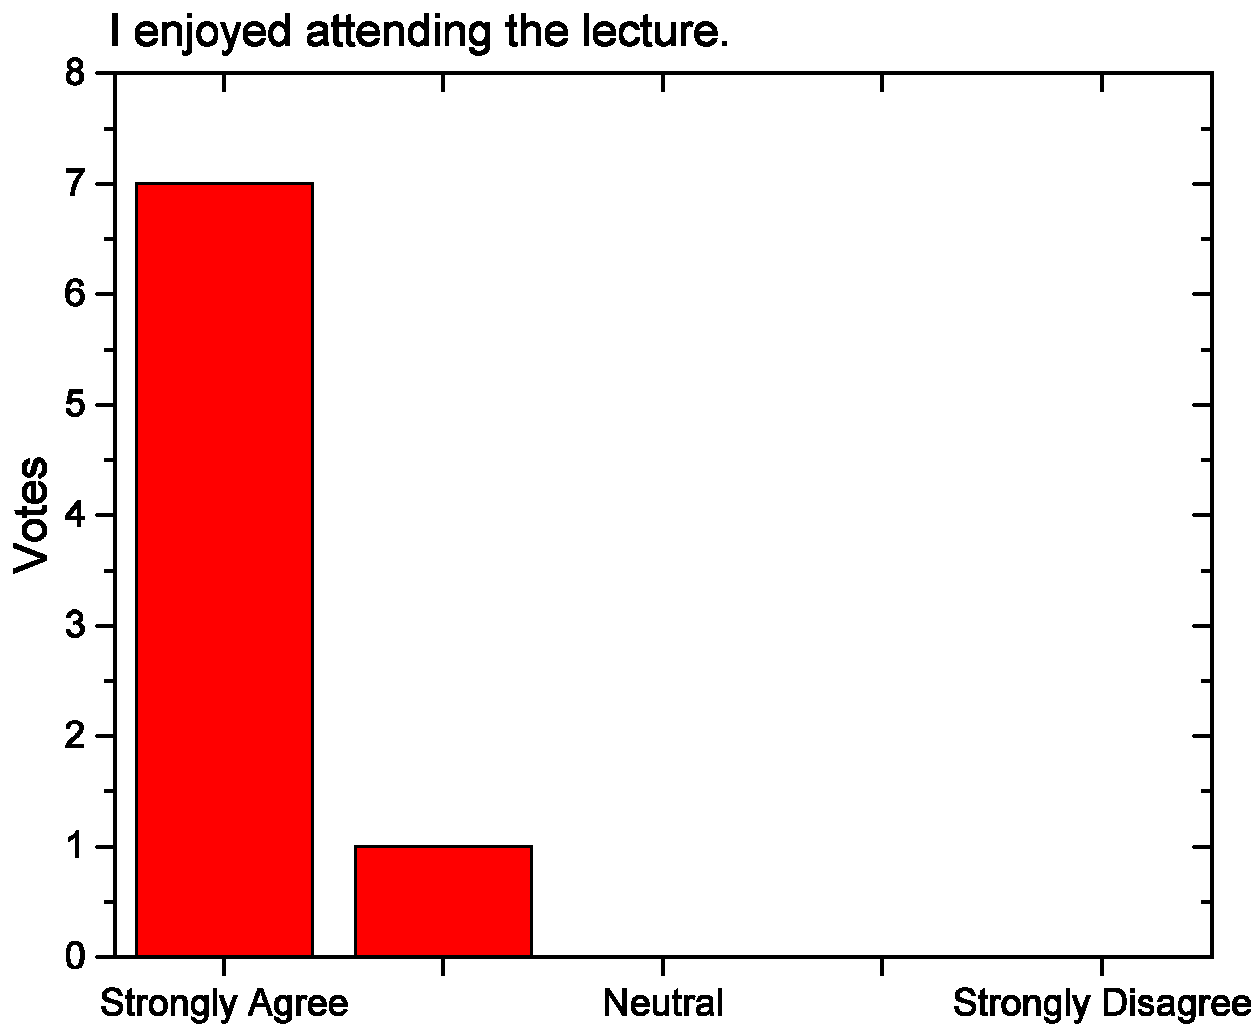
\includegraphics[height=50mm]{figures/n/Graph22.pdf}}
      {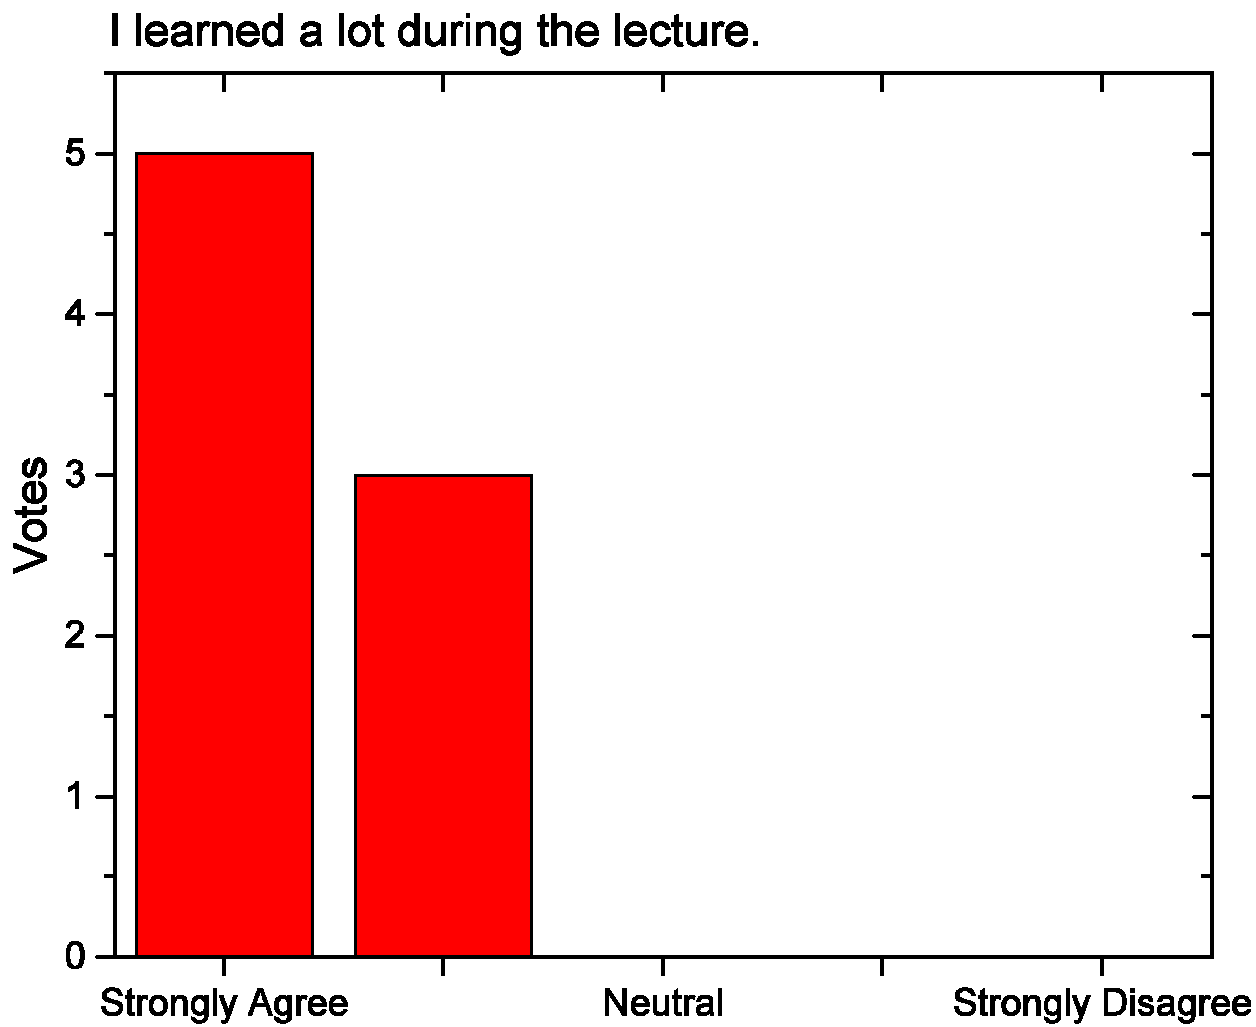
\includegraphics[height=50mm]{figures/n/Graph23.pdf}}
  \end{minipage}\quad
  \begin{minipage}{.48\linewidth}
    \centering
      {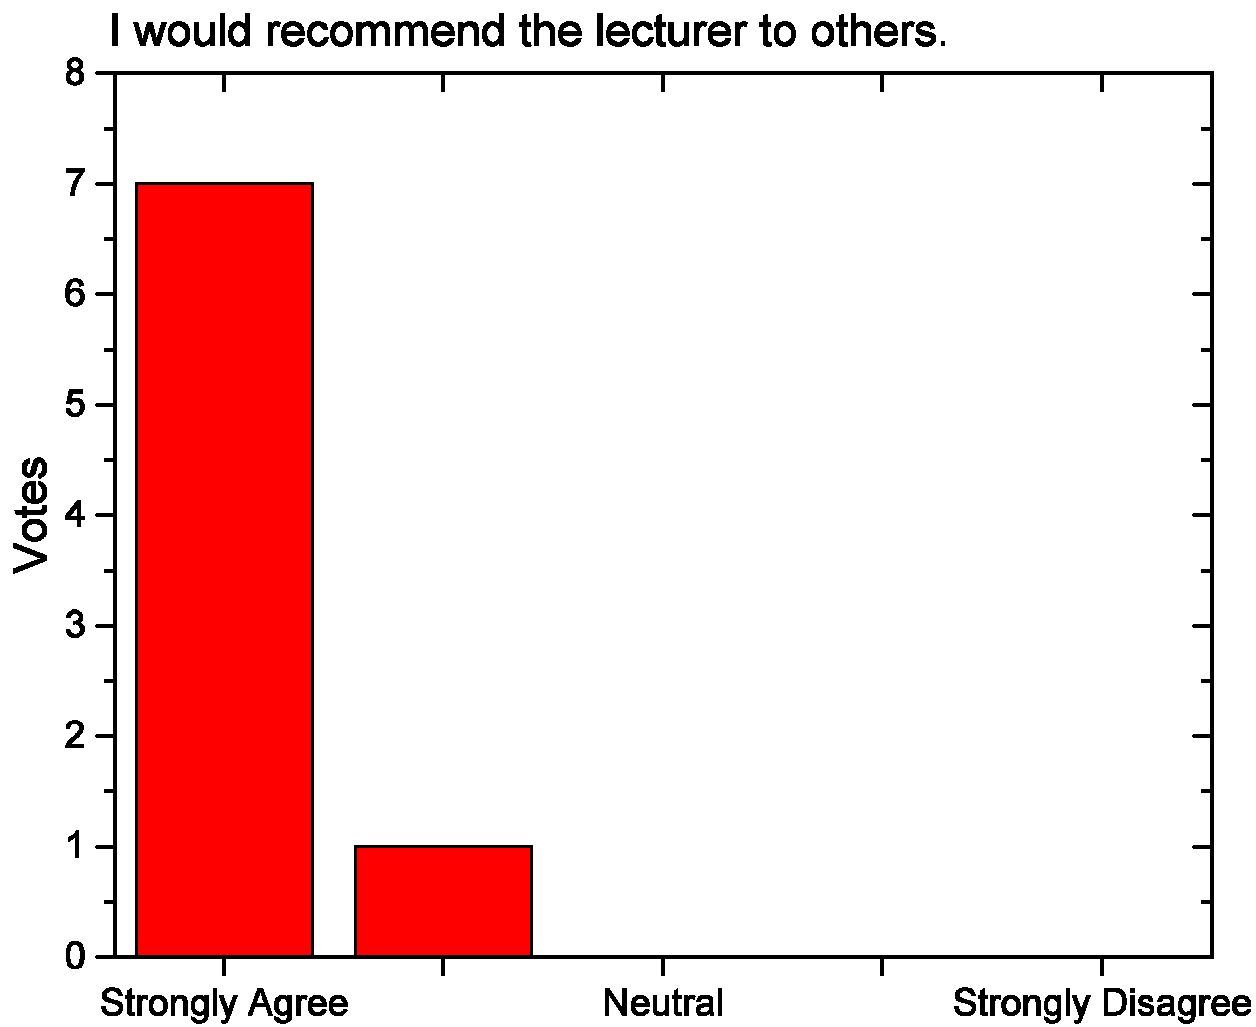
\includegraphics[height=50mm]{figures/n/Graph24.pdf}}
      {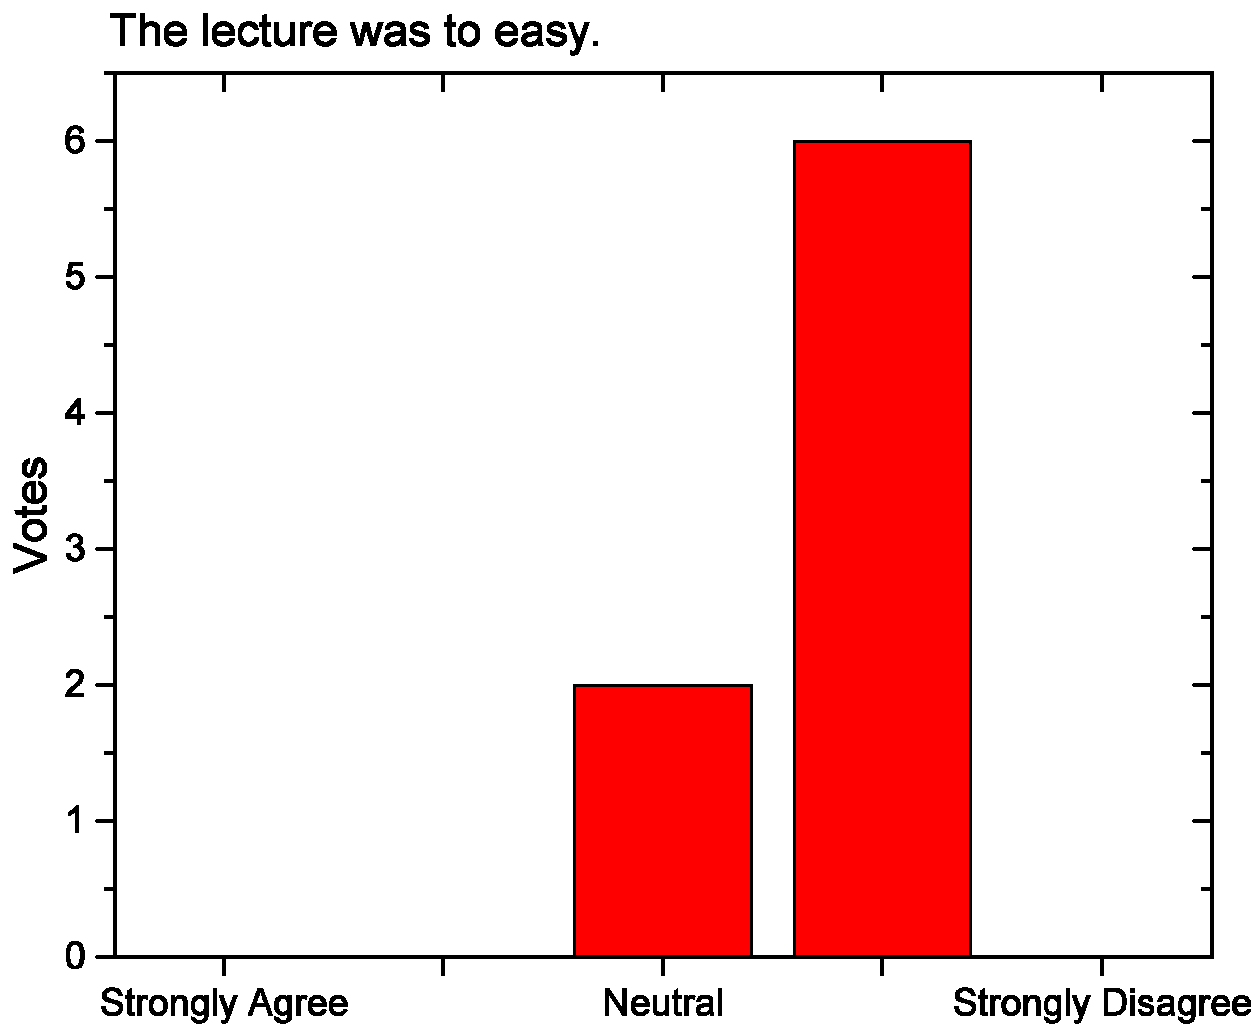
\includegraphics[height=50mm]{figures/n/Graph25.pdf}}
      {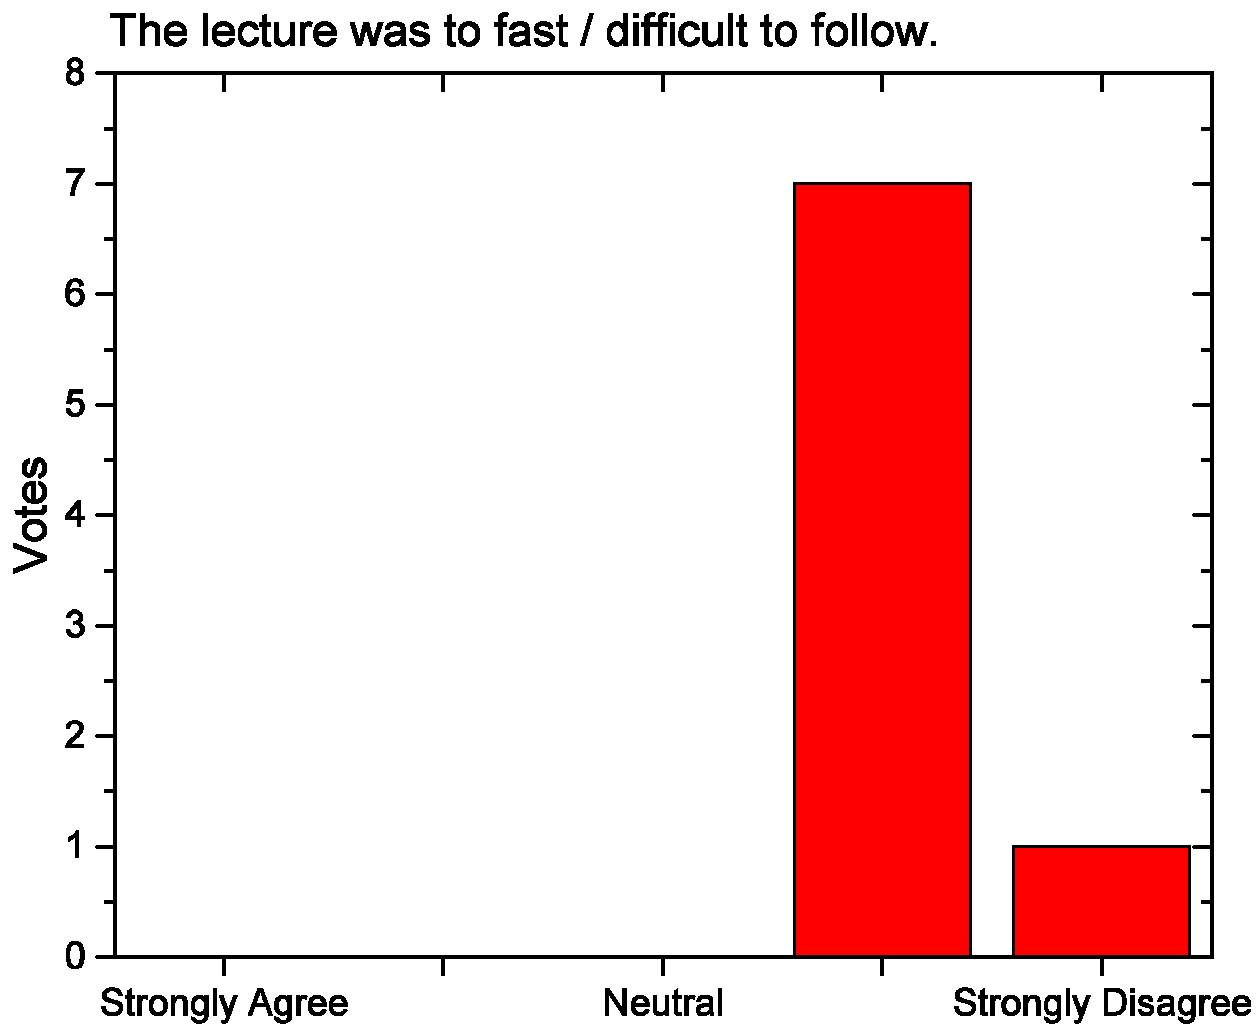
\includegraphics[height=50mm]{figures/n/Graph26.pdf}}
  \end{minipage}
\end{figure}

\begin{figure}[H]
  \begin{minipage}{.48\linewidth}
    \centering
      {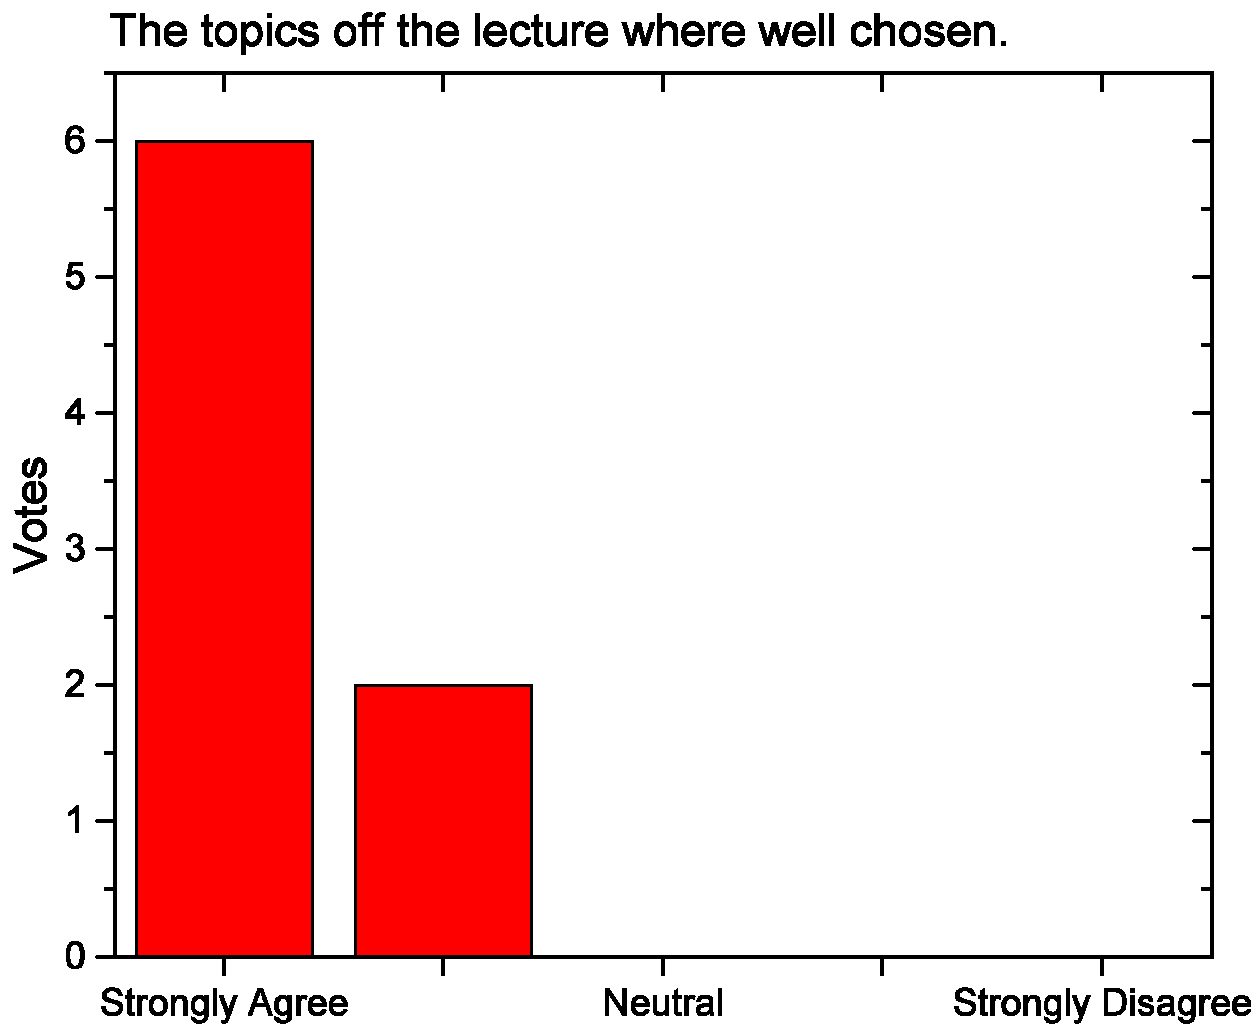
\includegraphics[height=50mm]{figures/n/Graph27.pdf}}
      {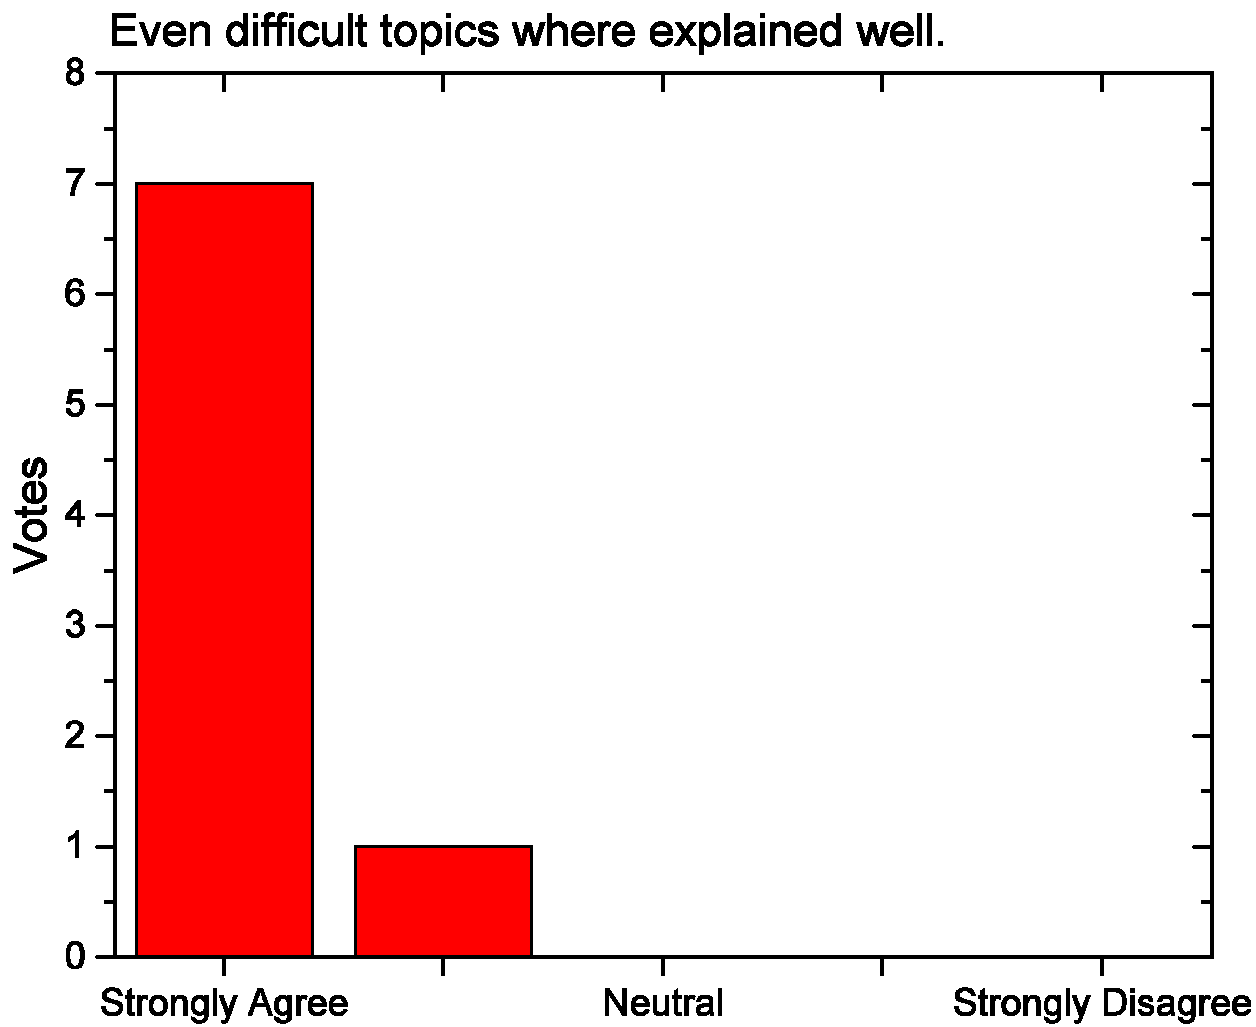
\includegraphics[height=50mm]{figures/n/Graph28.pdf}}
  \end{minipage}\quad
  \begin{minipage}{.48\linewidth}
    \centering
      {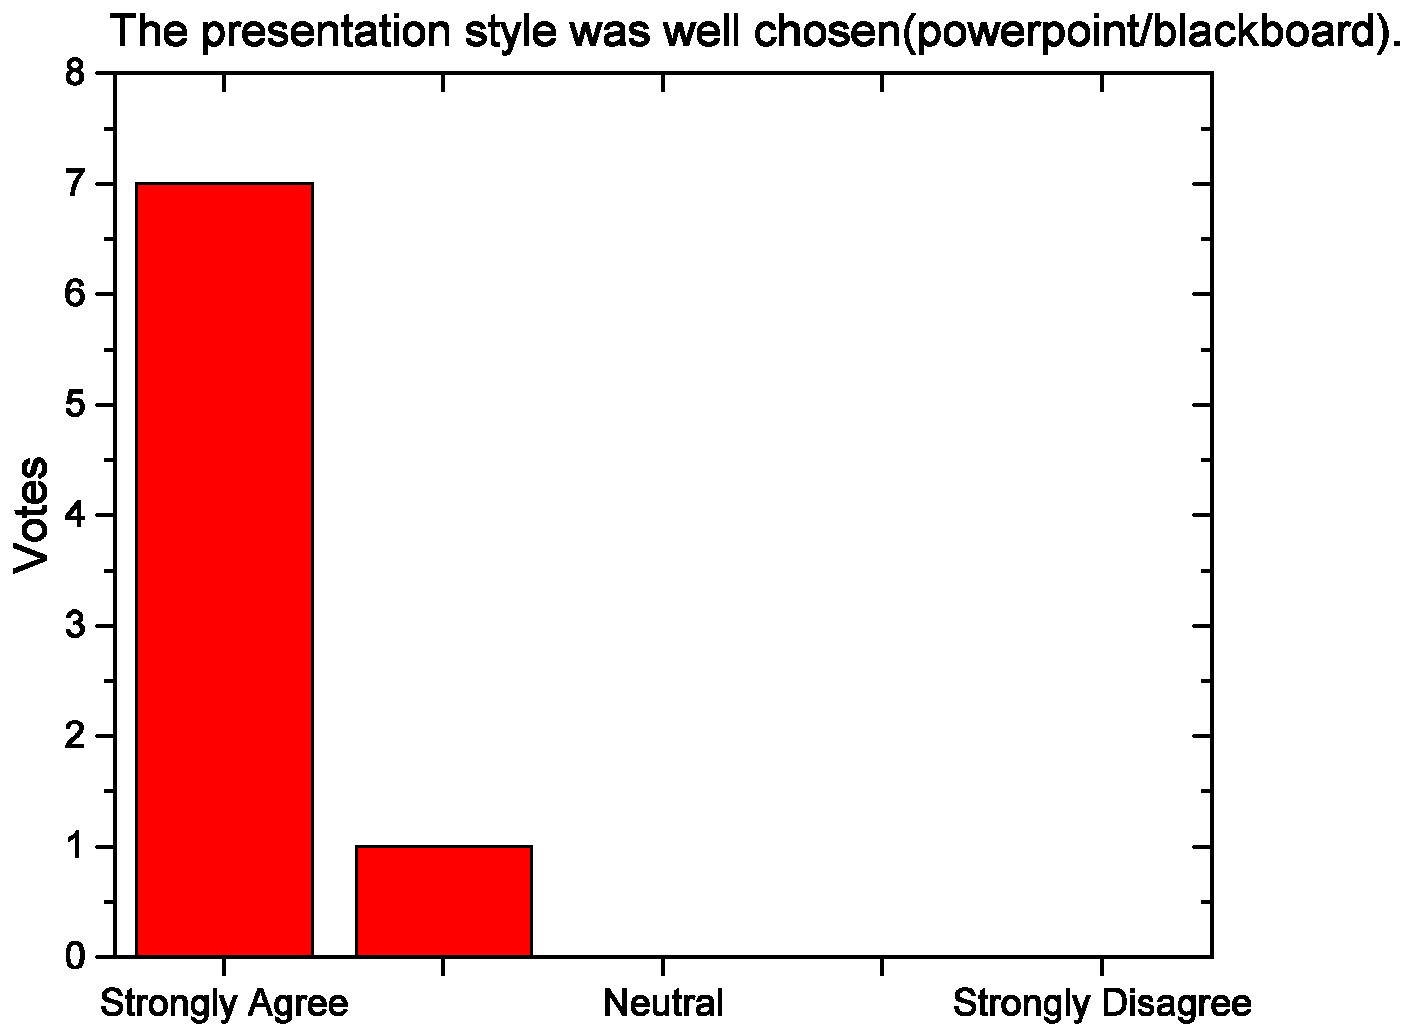
\includegraphics[height=50mm]{figures/n/Graph29.pdf}}
      {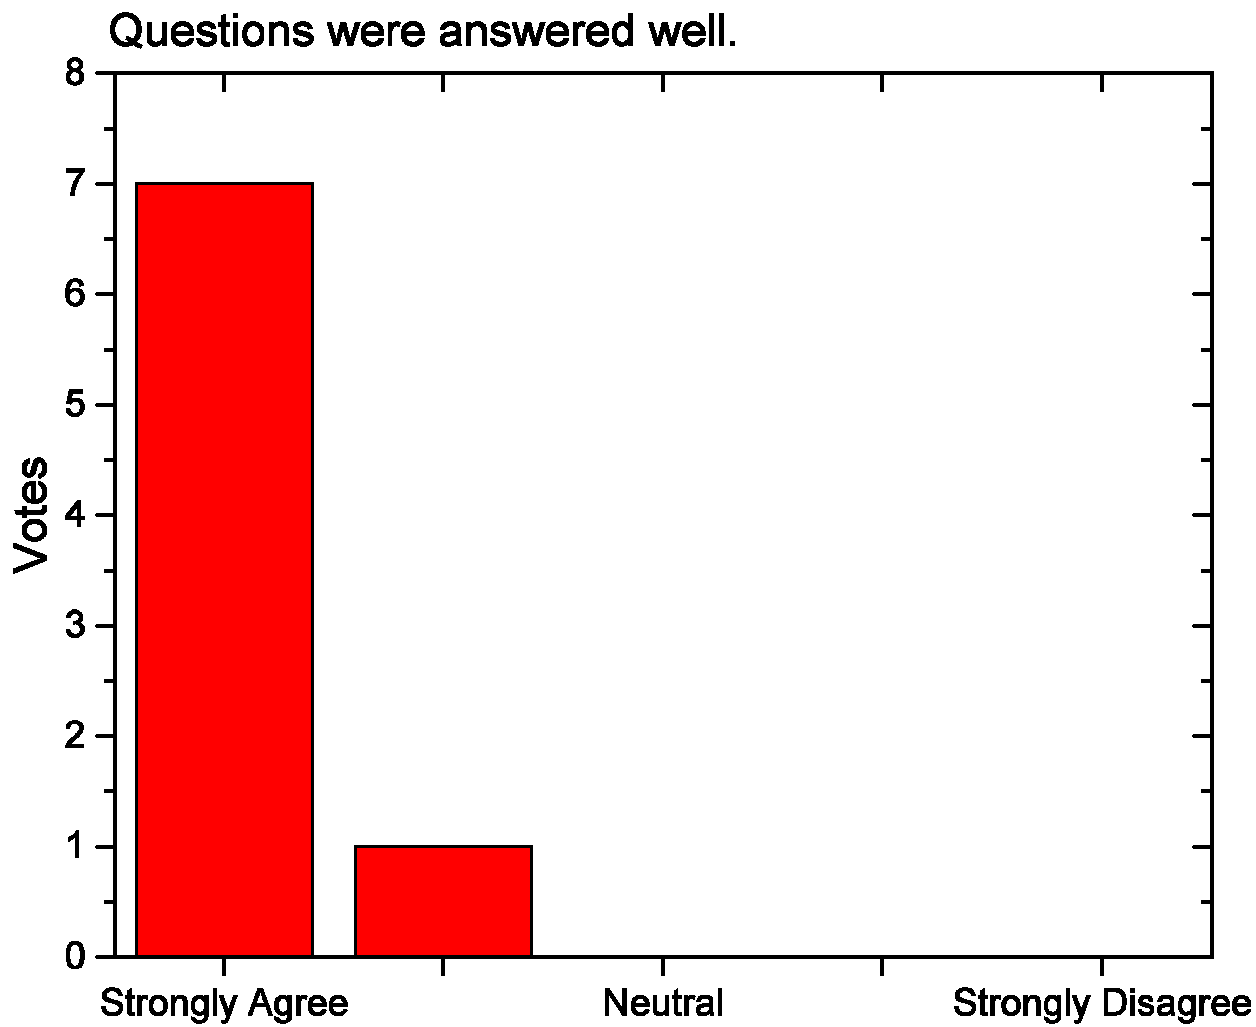
\includegraphics[height=50mm]{figures/n/Graph30.pdf}}
  \end{minipage}
\end{figure}

\subsubsection*{Comments}
-


\clearpage
\subsubsection{Genevieve Parmentier  --- Fascinating aspects of globular star clusters }
\pdfbookmark{B2 Genevieve Parmentier}{label:gp}
\begin{figure}[h!]
  \centering
  \begin{minipage}{.48\linewidth}
    \centering
      {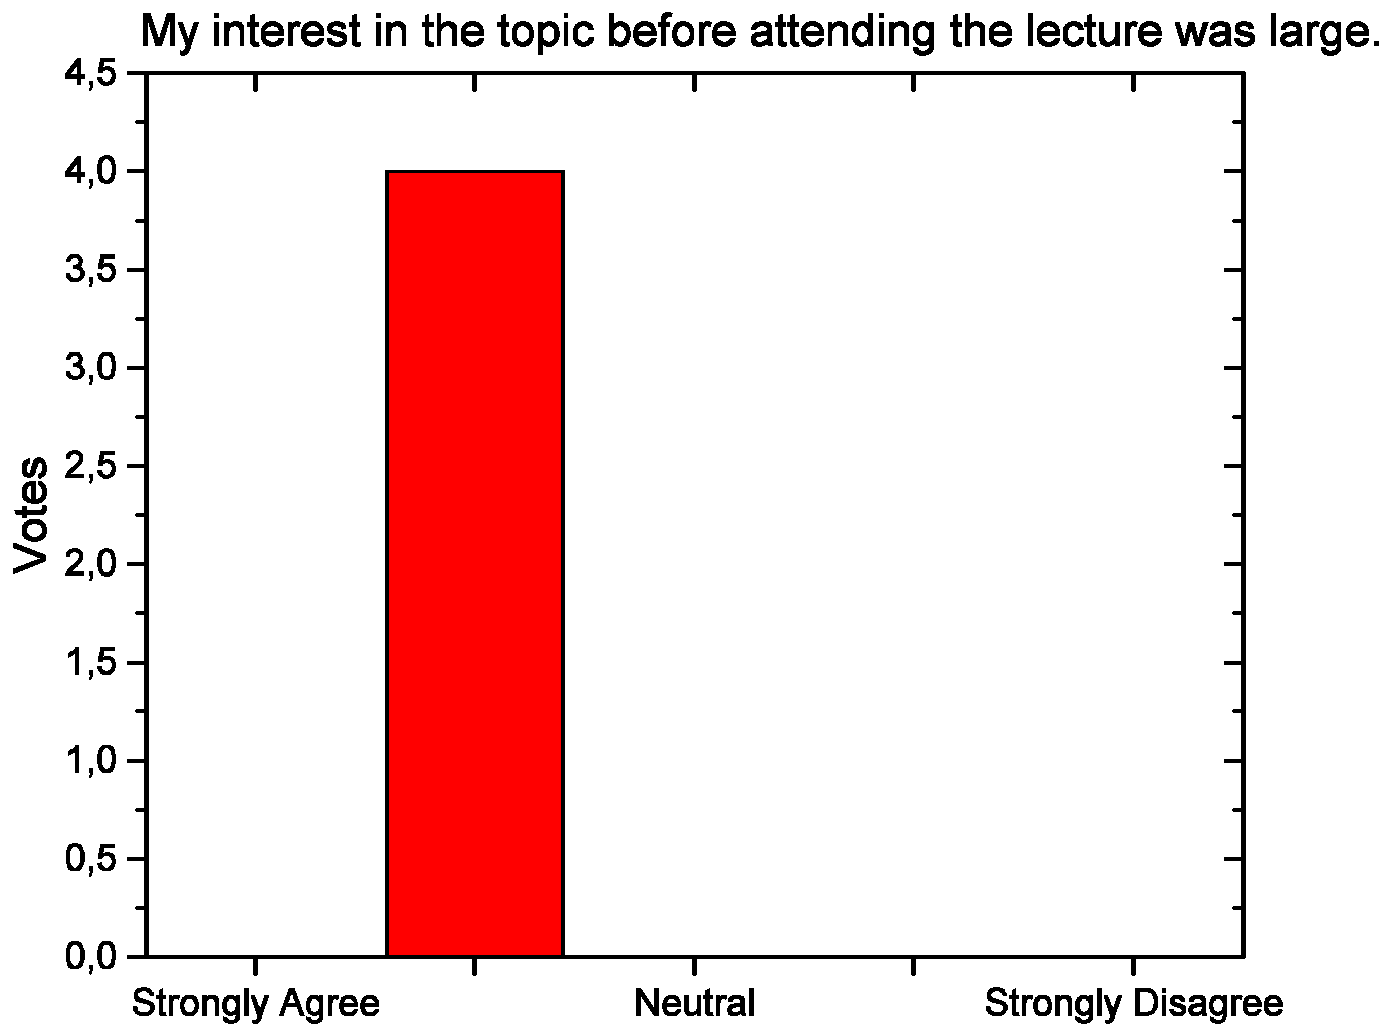
\includegraphics[height=50mm]{figures/n/Graph31.pdf}}
      {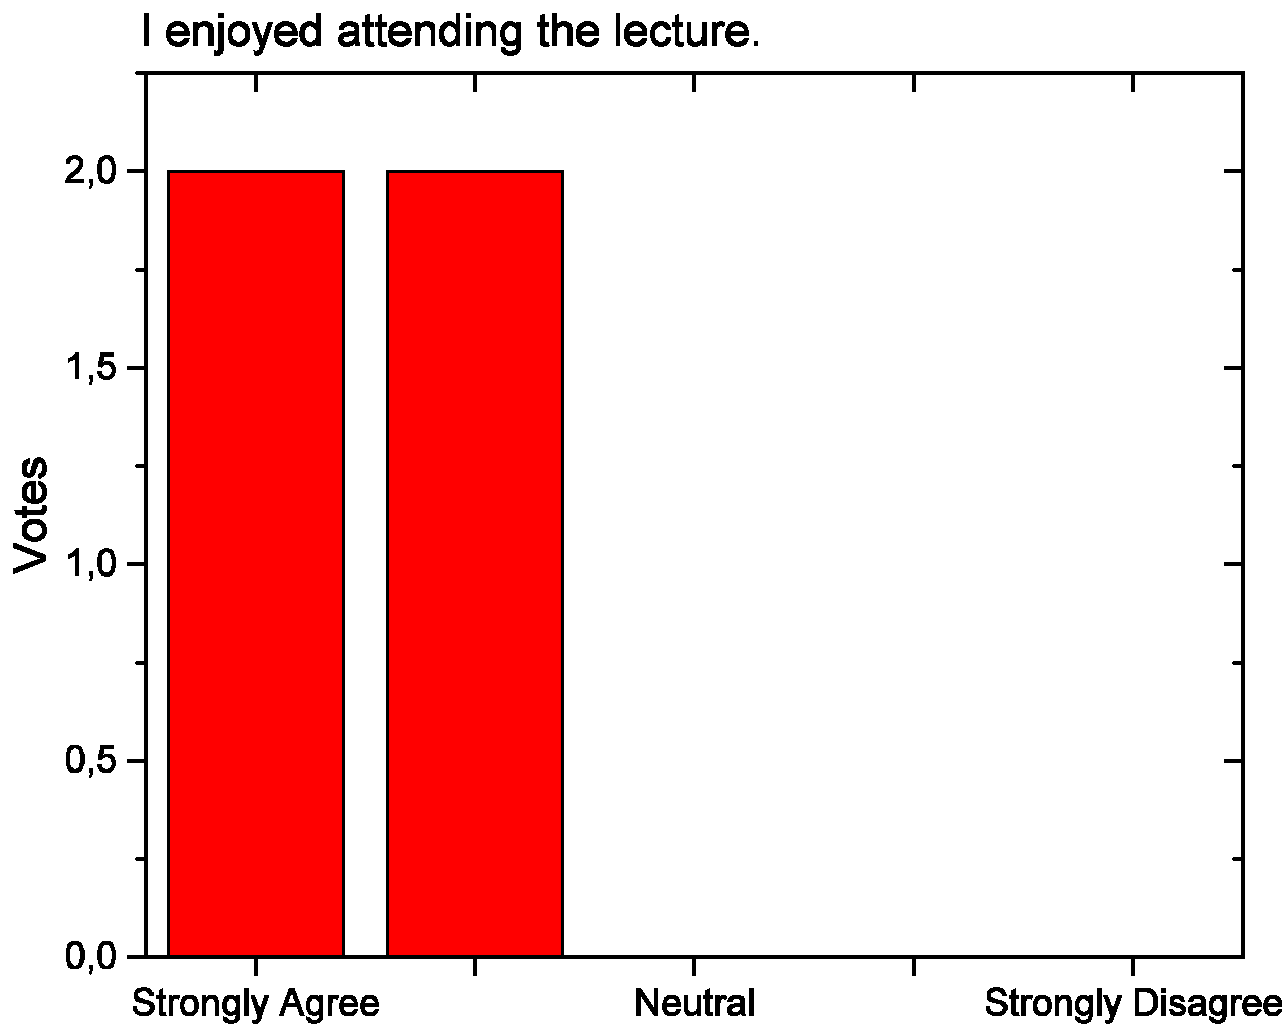
\includegraphics[height=50mm]{figures/n/Graph32.pdf}}
      {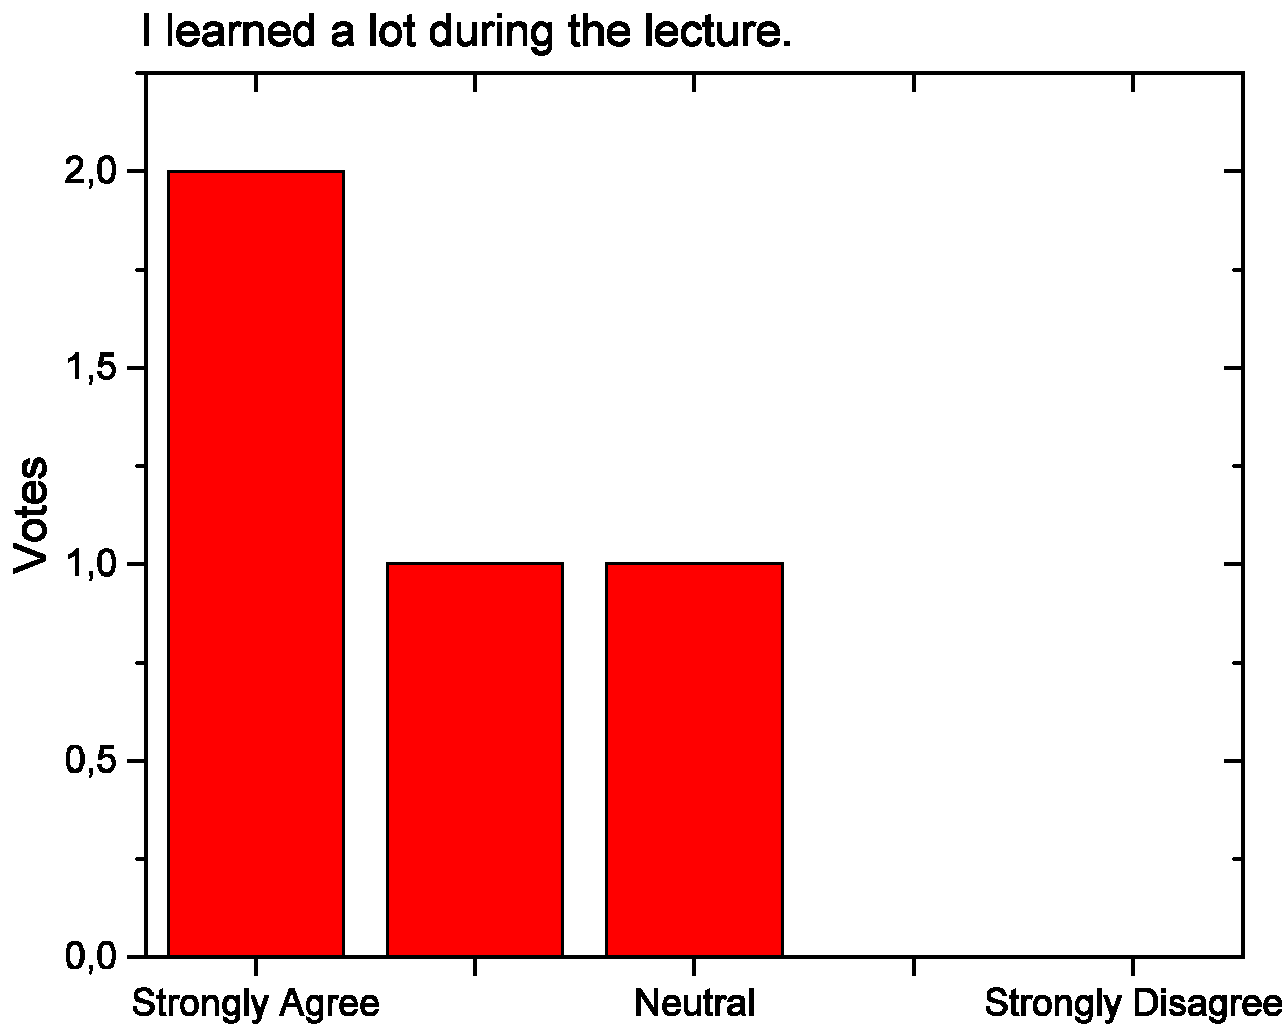
\includegraphics[height=50mm]{figures/n/Graph33.pdf}}
  \end{minipage}\quad
  \begin{minipage}{.48\linewidth}
    \centering
      {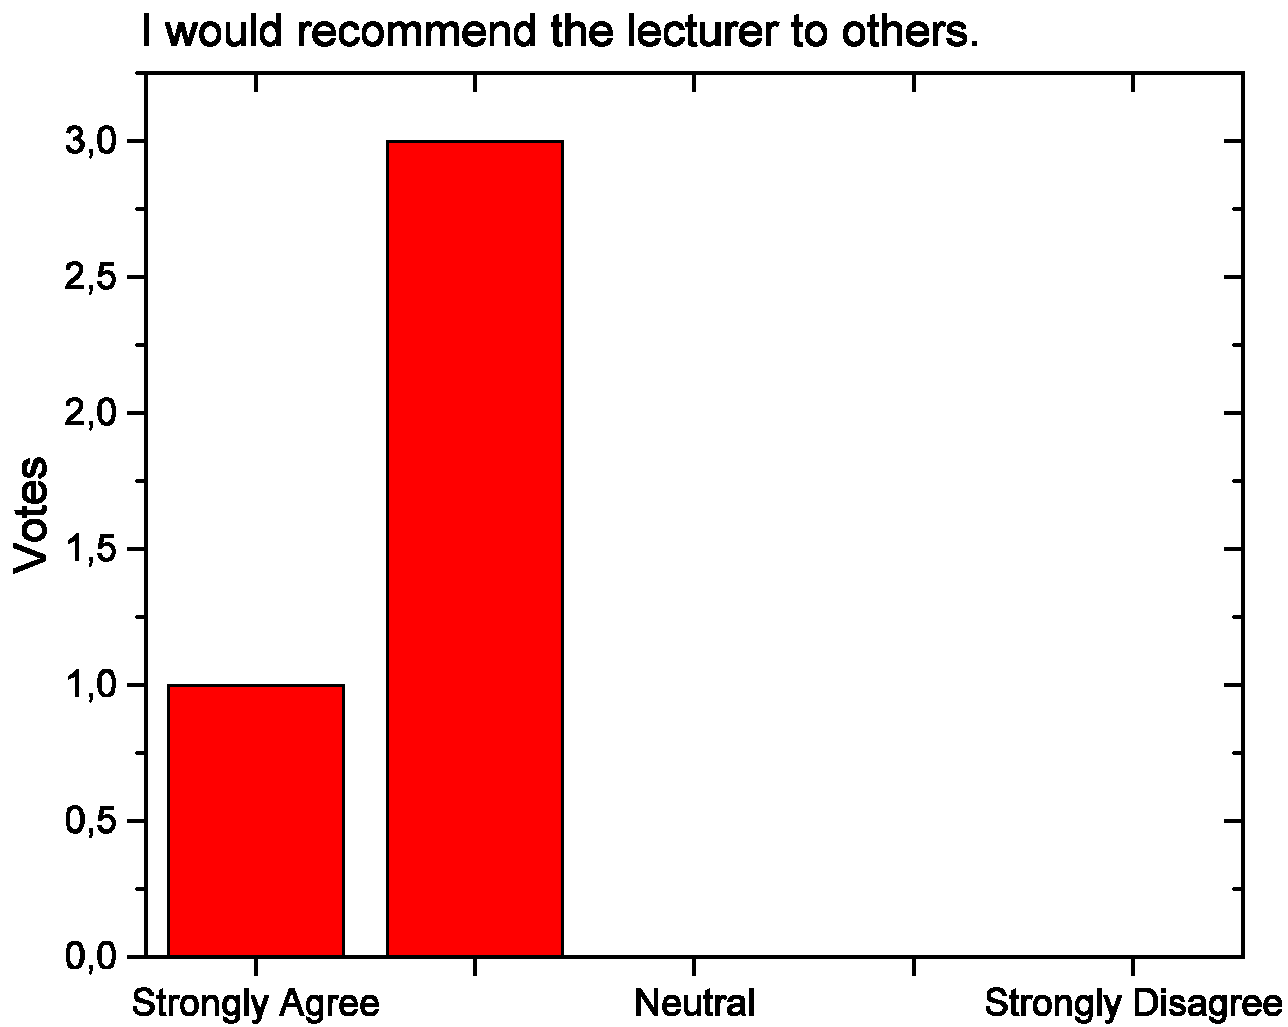
\includegraphics[height=50mm]{figures/n/Graph34.pdf}}
      {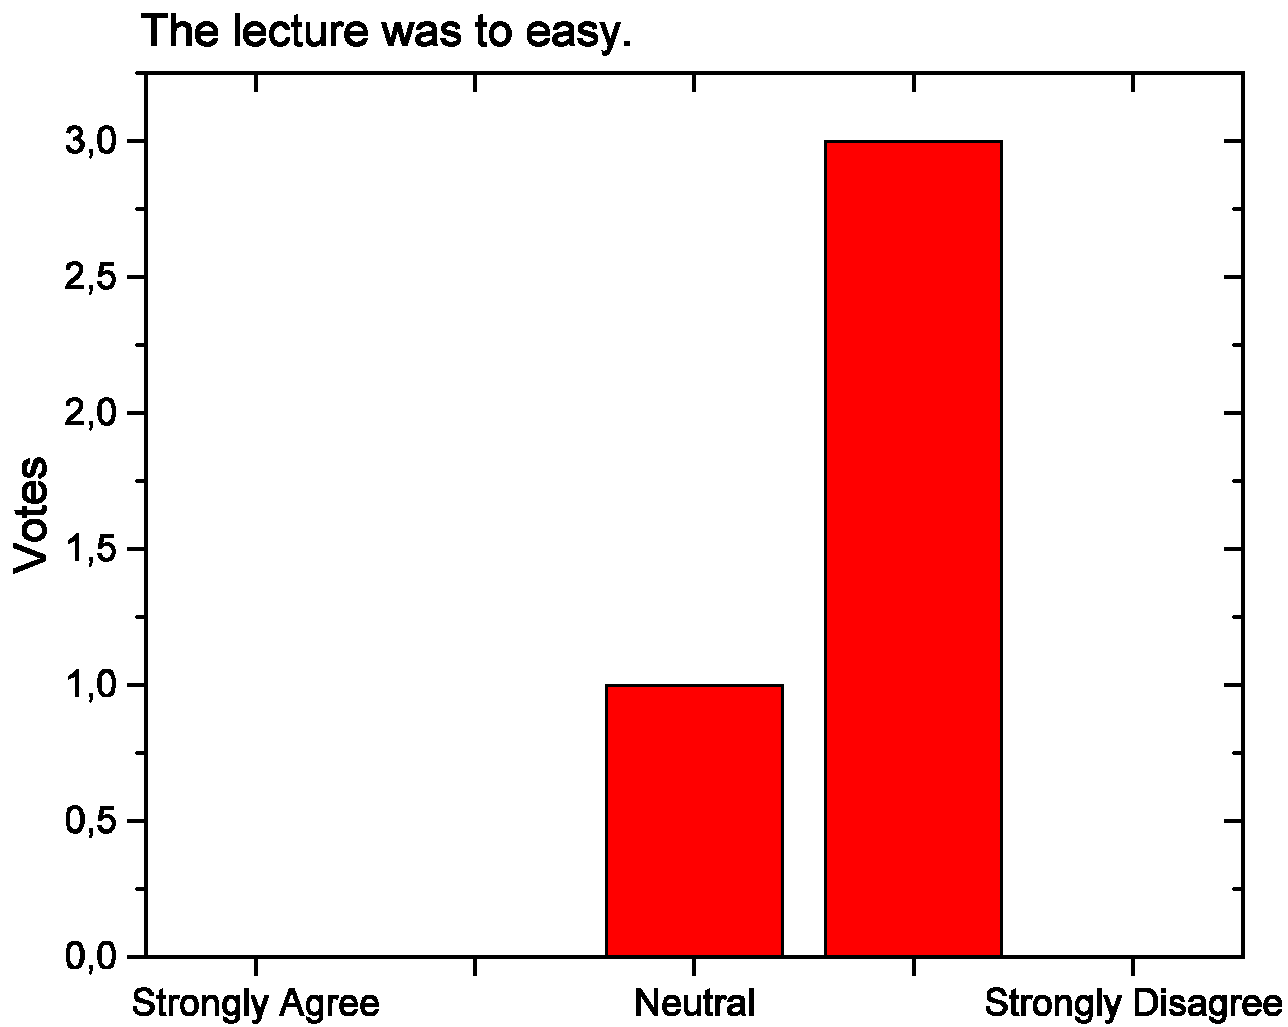
\includegraphics[height=50mm]{figures/n/Graph35.pdf}}
      {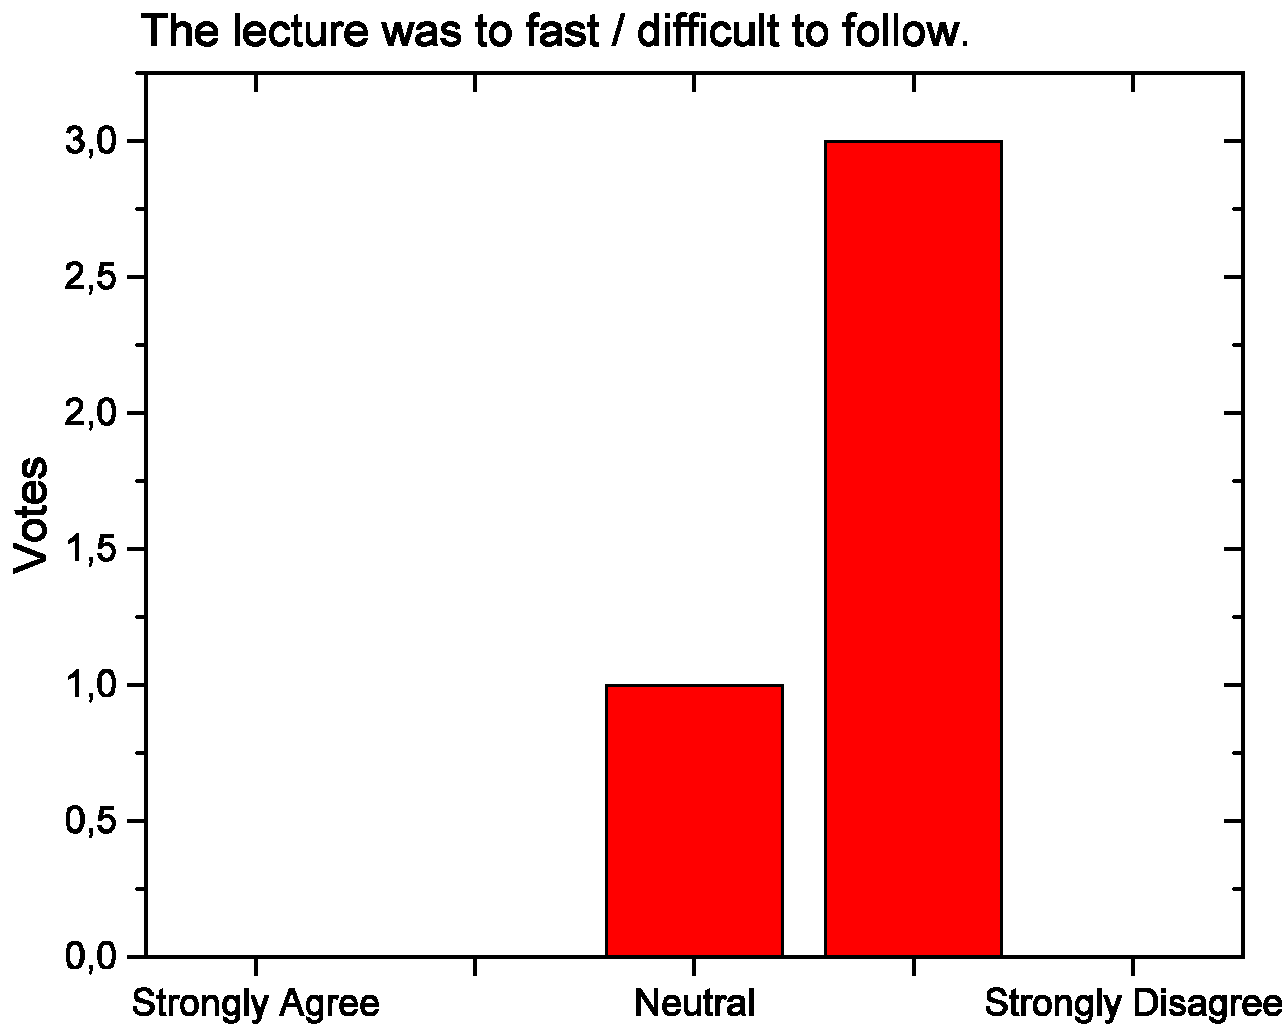
\includegraphics[height=50mm]{figures/n/Graph36.pdf}}
  \end{minipage}
\end{figure}

\begin{figure}[H]
  \begin{minipage}{.48\linewidth}
    \centering
      {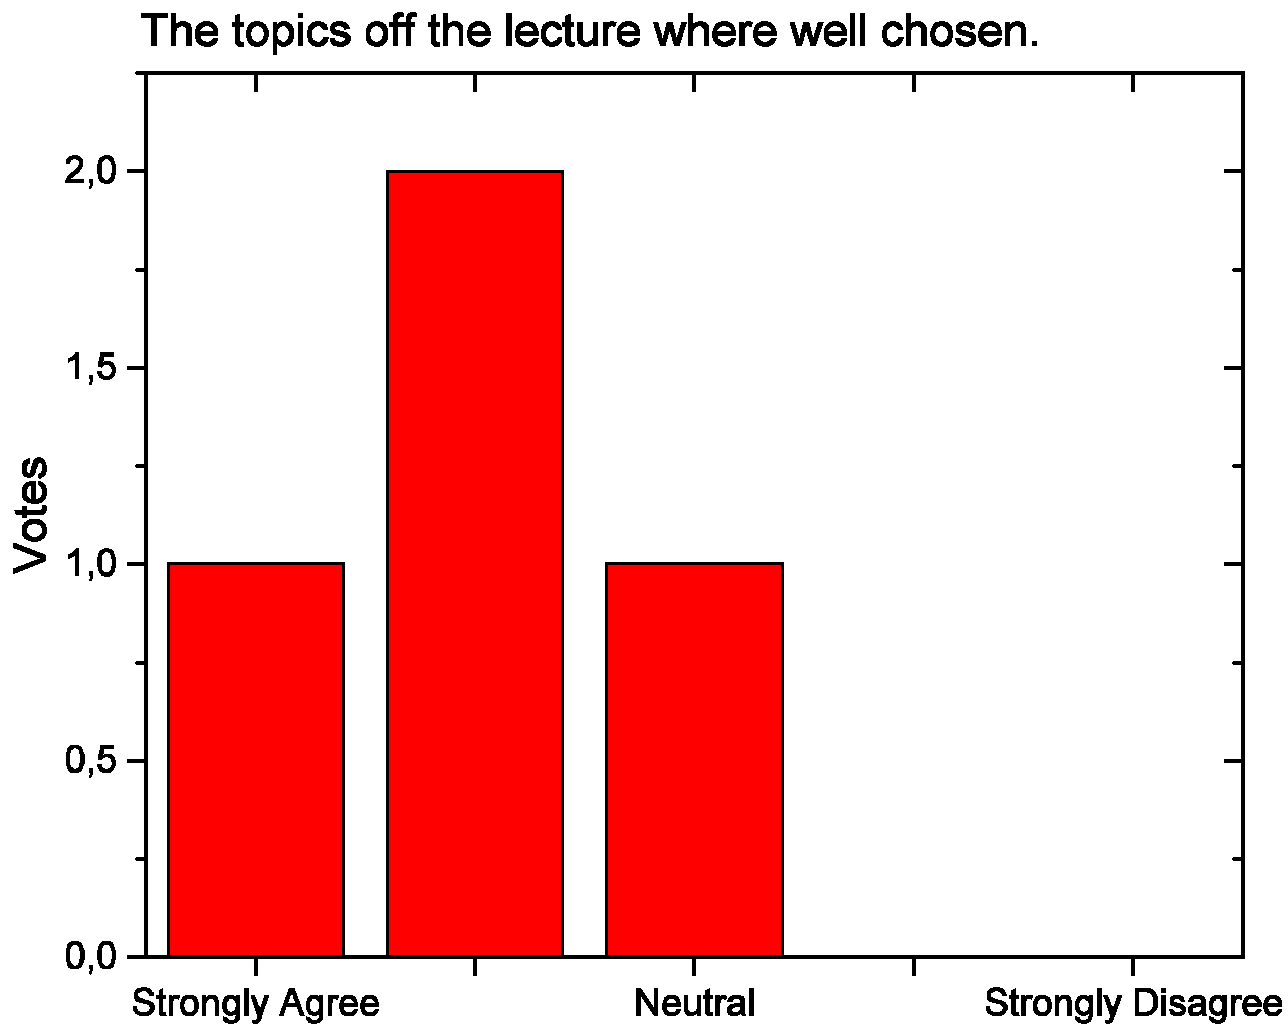
\includegraphics[height=50mm]{figures/n/Graph37.pdf}}
      {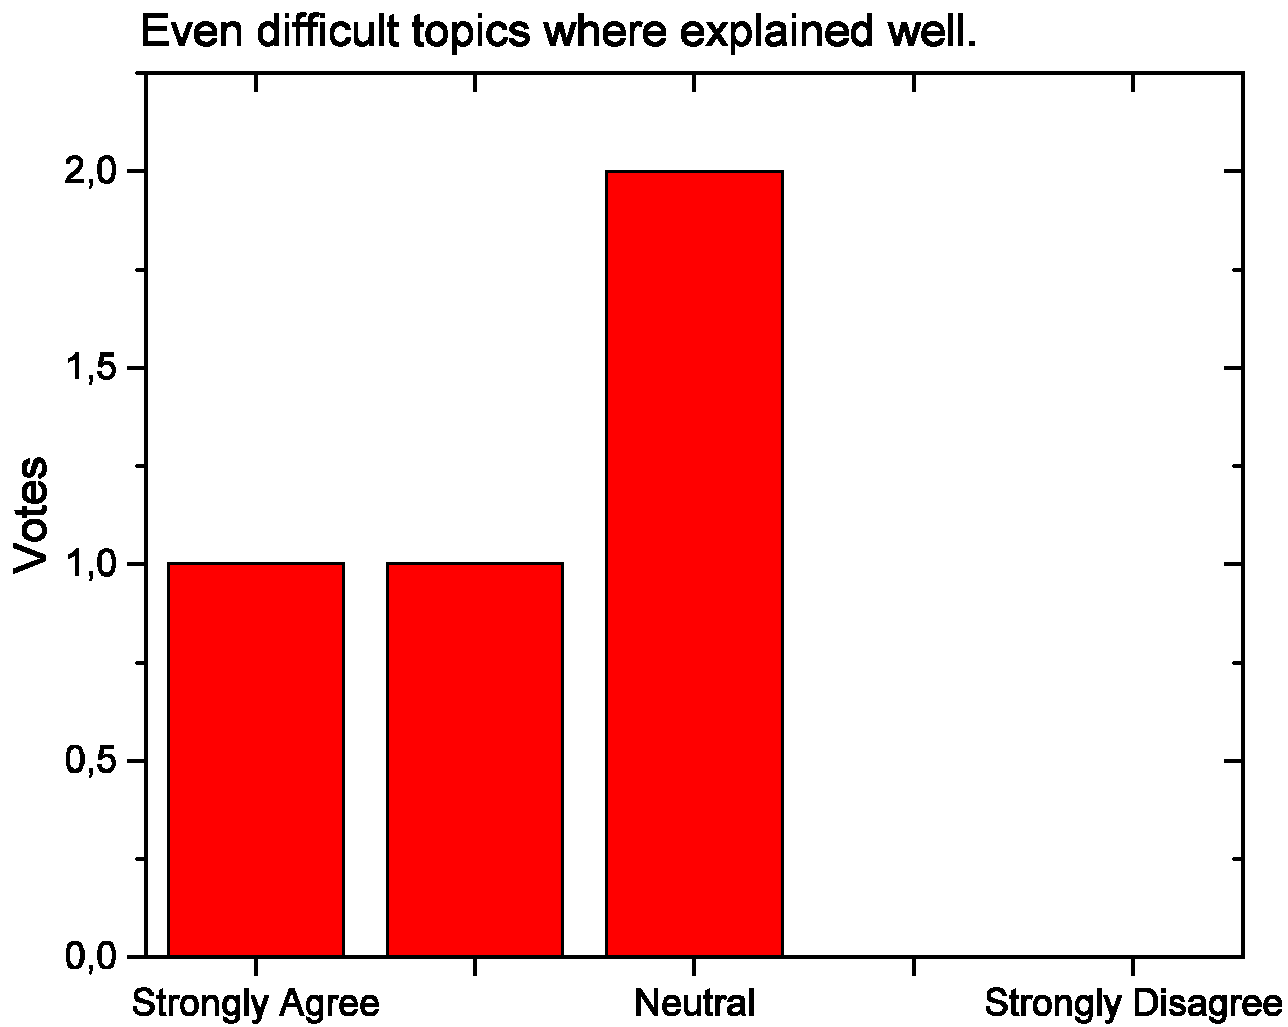
\includegraphics[height=50mm]{figures/n/Graph38.pdf}}
  \end{minipage}\quad
  \begin{minipage}{.48\linewidth}
    \centering
      {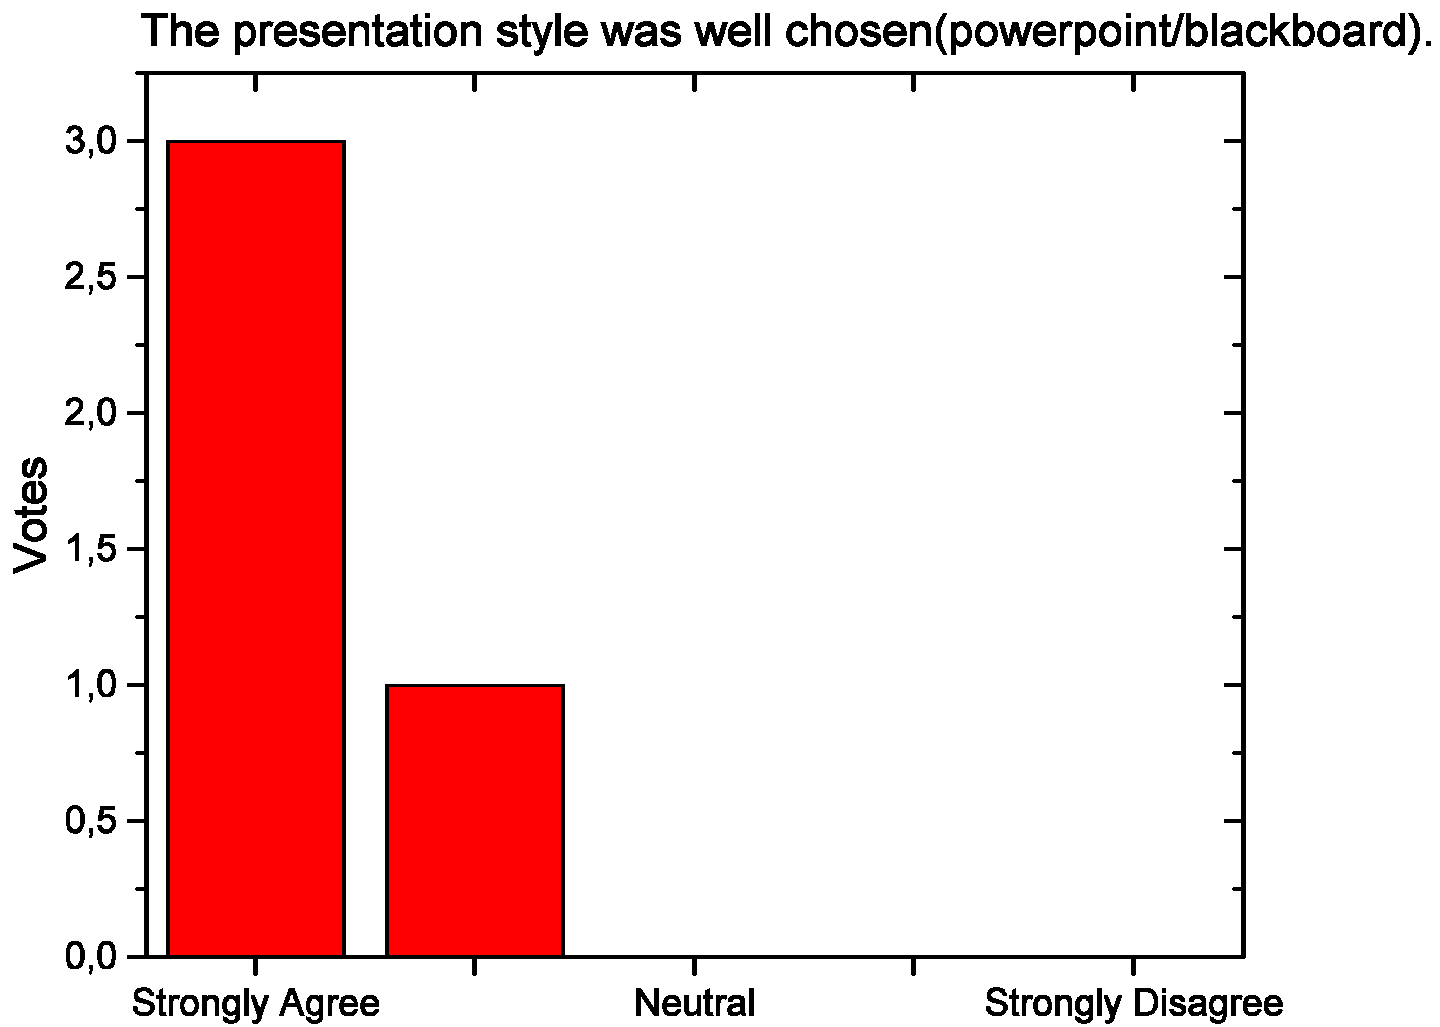
\includegraphics[height=50mm]{figures/n/Graph39.pdf}}
      {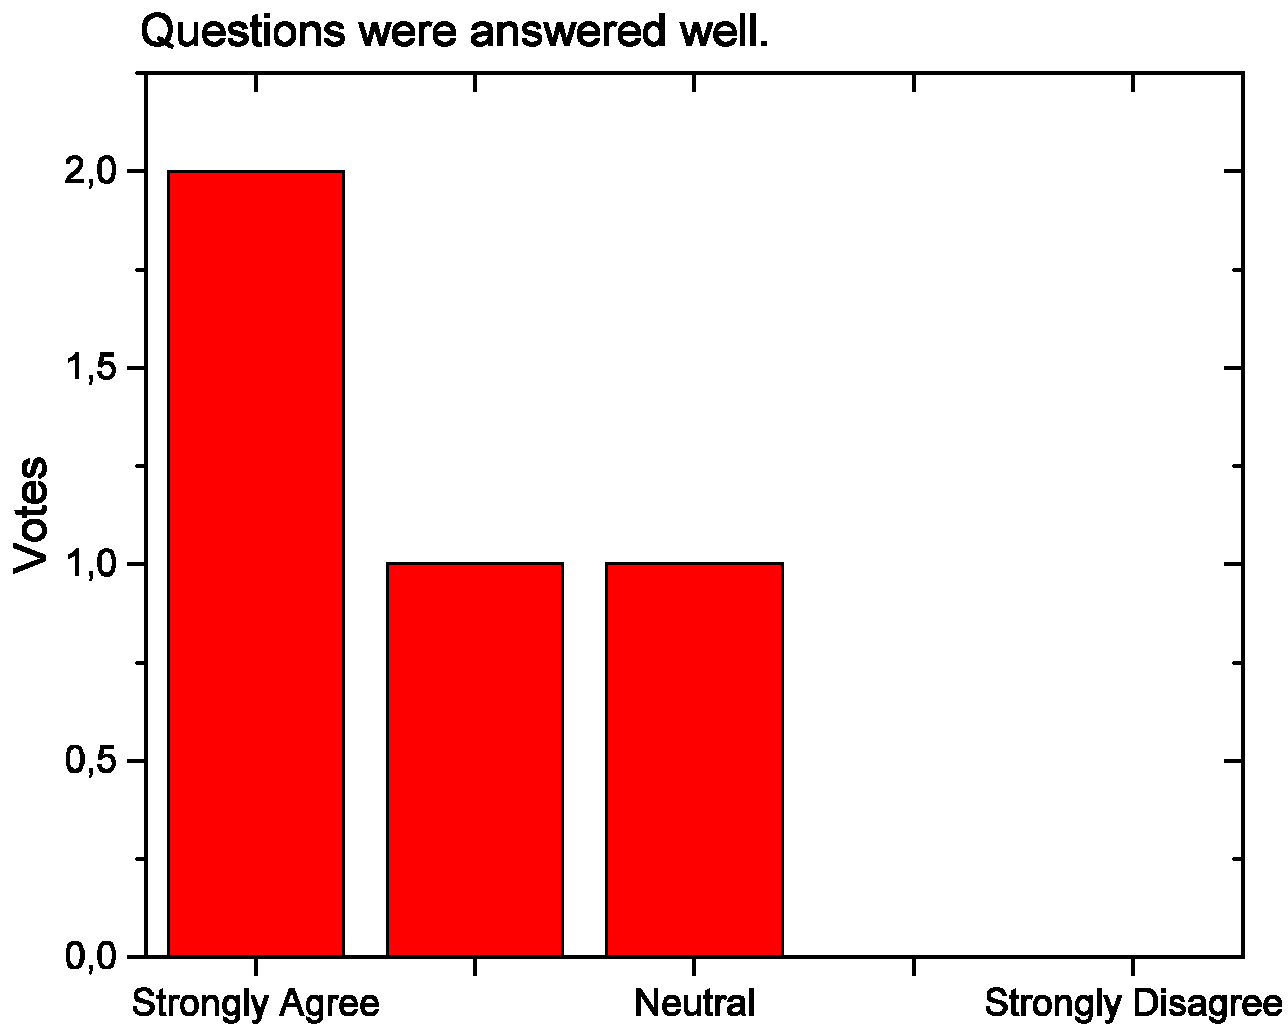
\includegraphics[height=50mm]{figures/n/Graph40.pdf}}
  \end{minipage}
\end{figure}
\subsubsection*{Comments}
-
\newpage

\subsubsection{Zoltan Harman  --- Quantum electrodynamics of bound systems}
\pdfbookmark{B2 Zoltan Harman}{label:zh}
\begin{figure}[h!]
  \centering
  \begin{minipage}{.48\linewidth}
    \centering
      {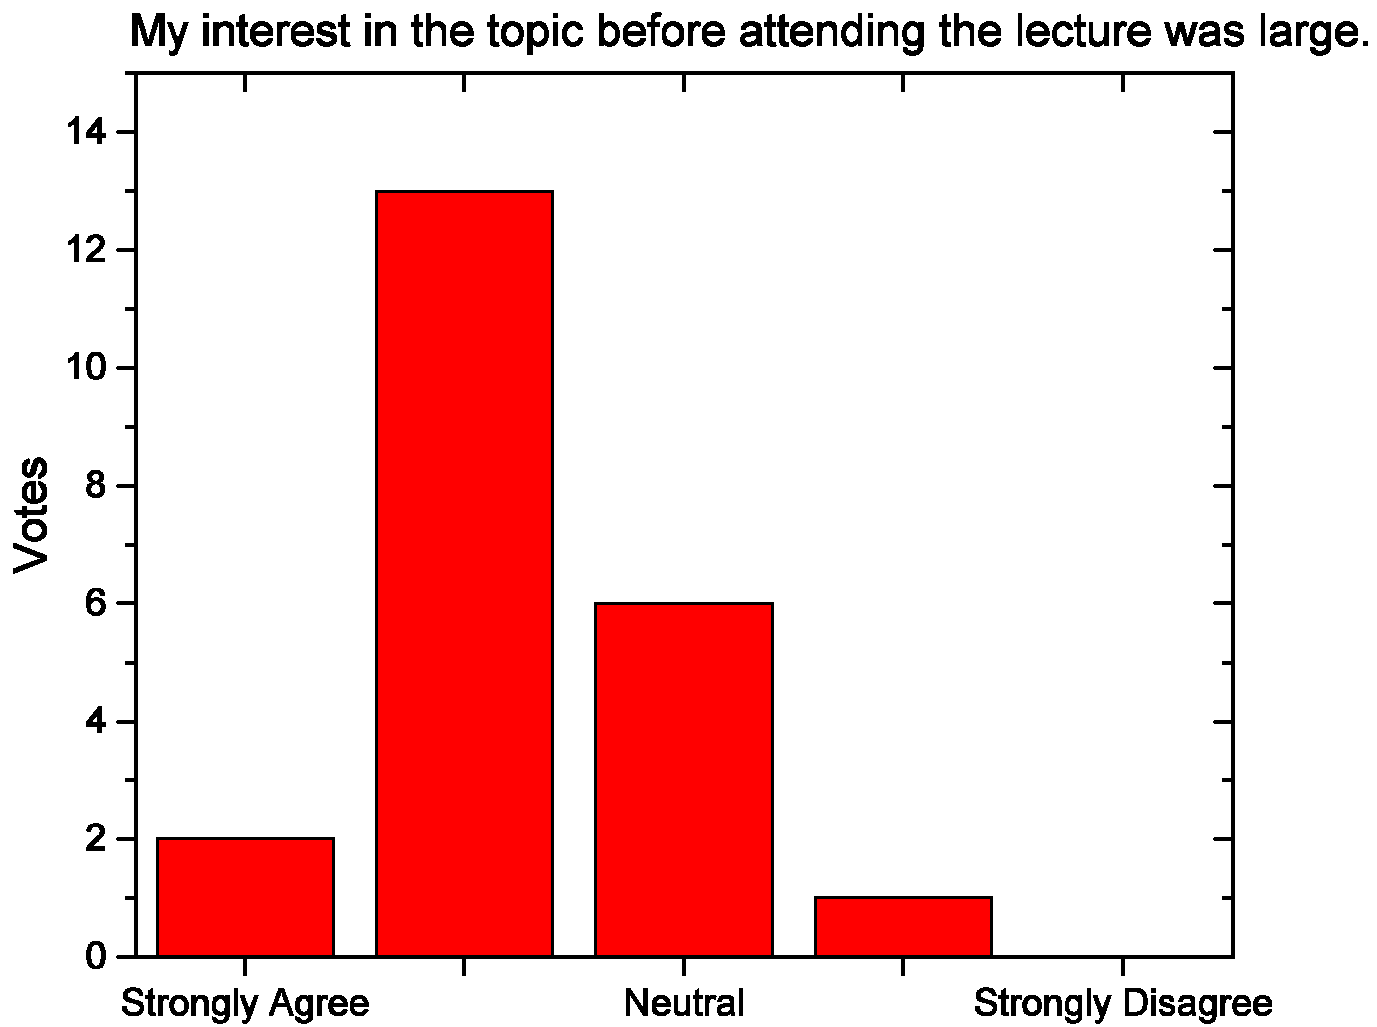
\includegraphics[height=50mm]{figures/n/Graph41.pdf}}
      {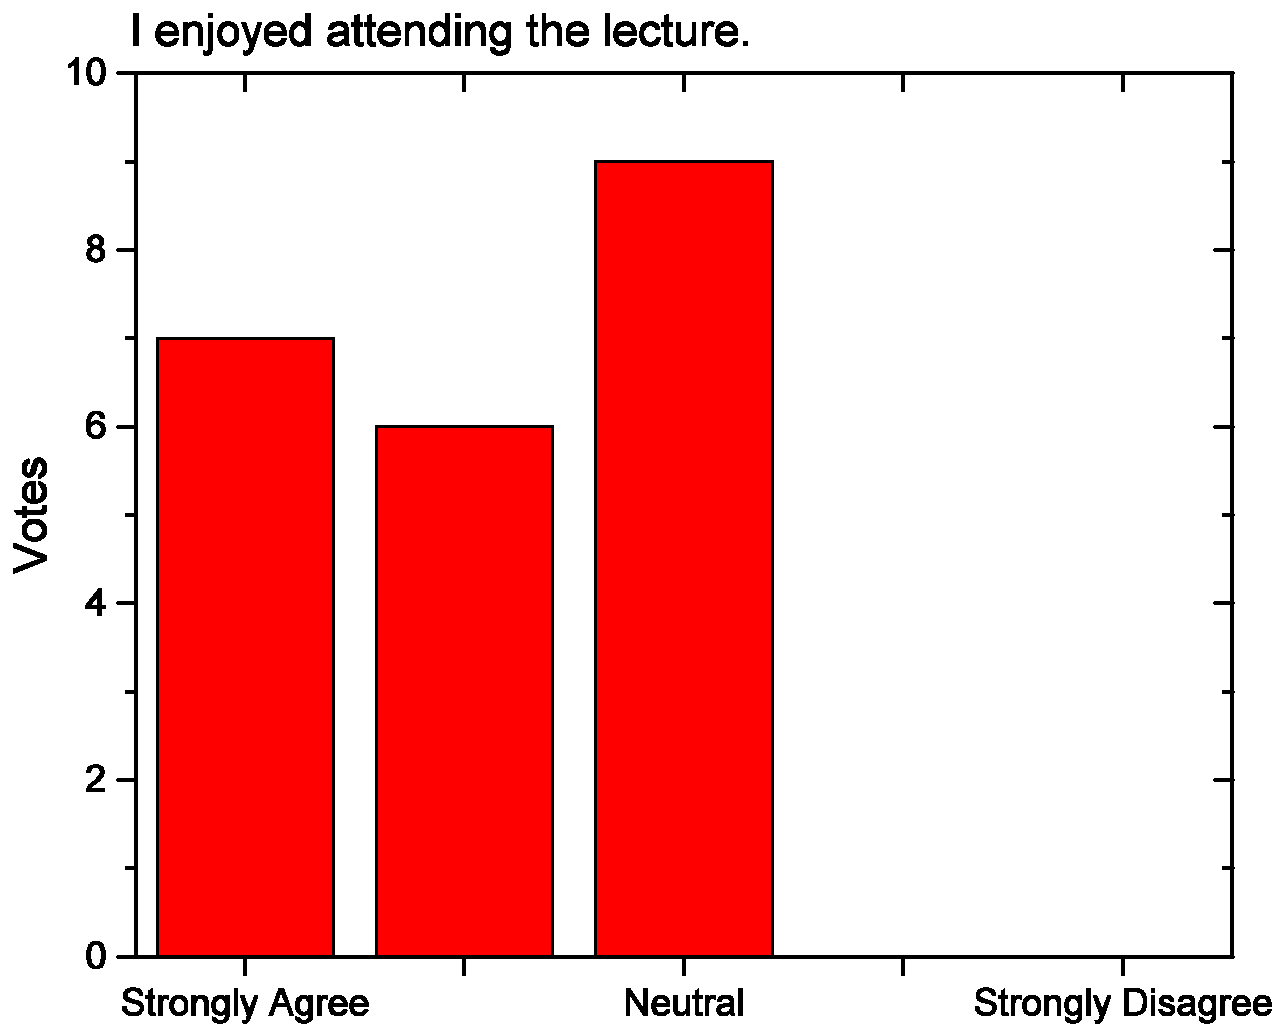
\includegraphics[height=50mm]{figures/n/Graph42.pdf}}
      {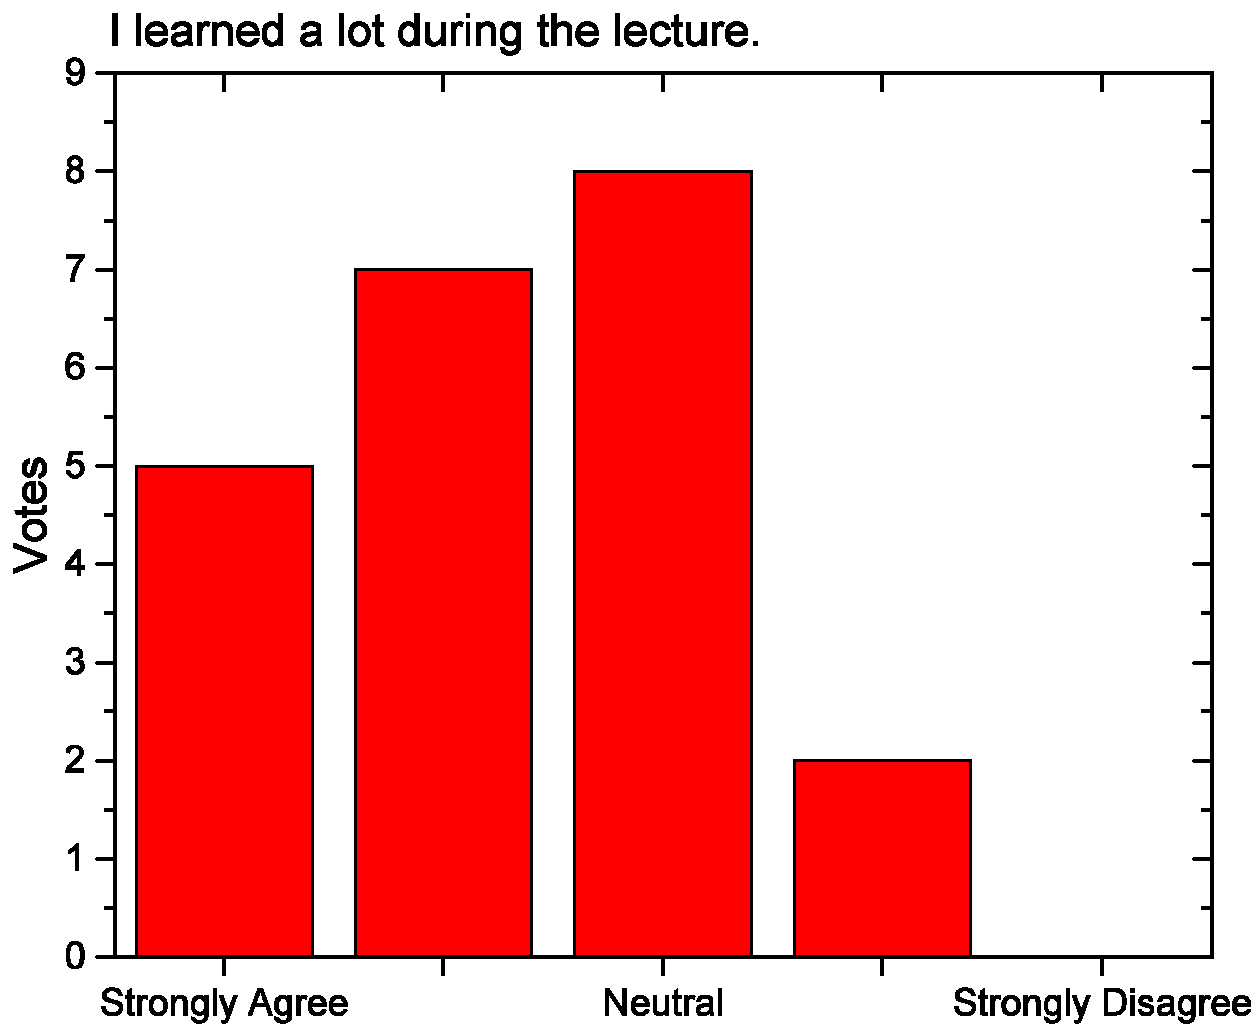
\includegraphics[height=50mm]{figures/n/Graph43.pdf}}
  \end{minipage}\quad
  \begin{minipage}{.48\linewidth}
    \centering
      {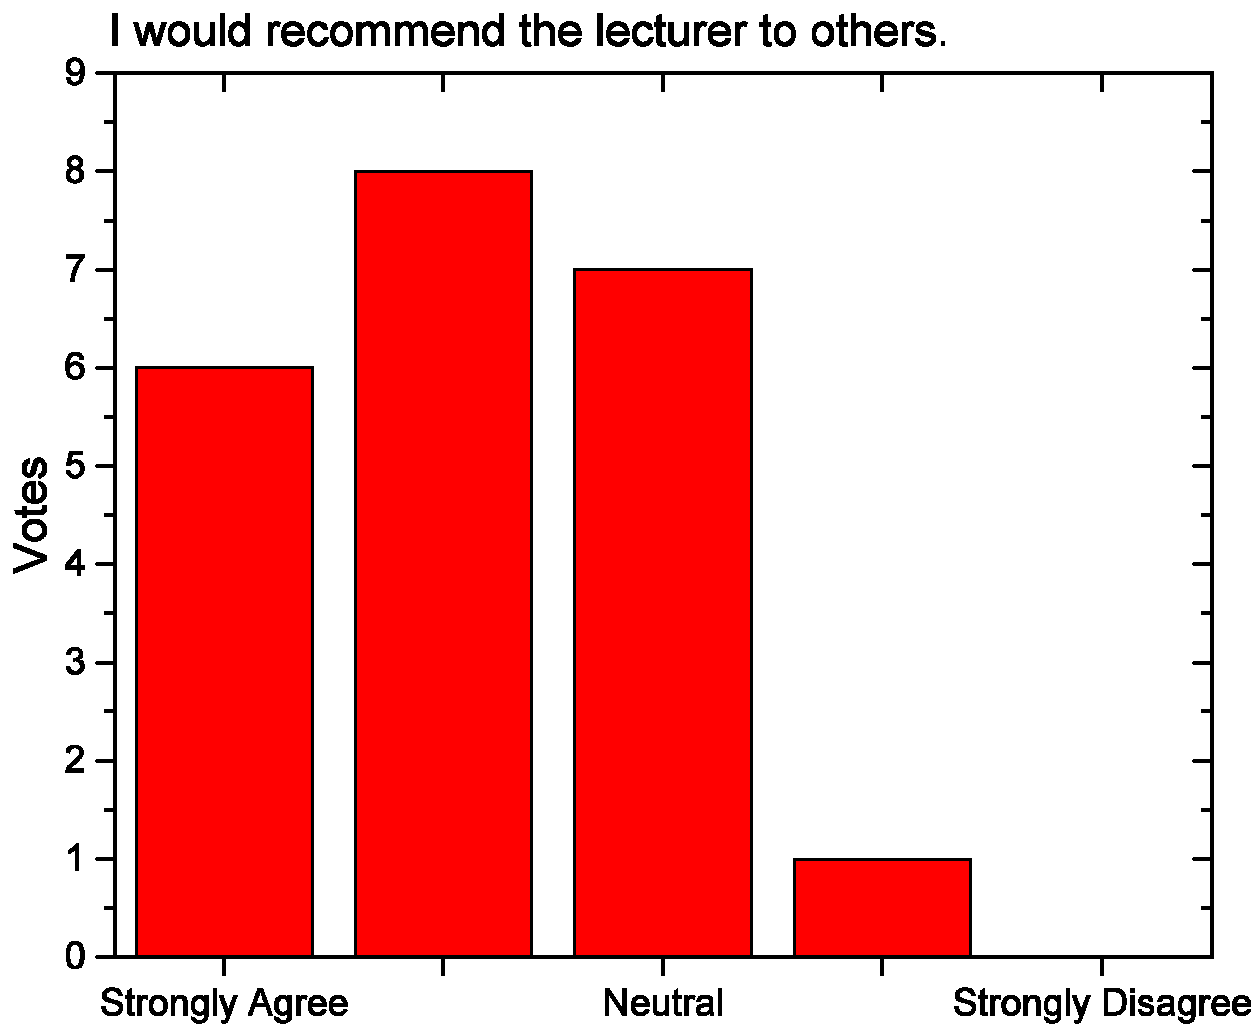
\includegraphics[height=50mm]{figures/n/Graph44.pdf}}
      {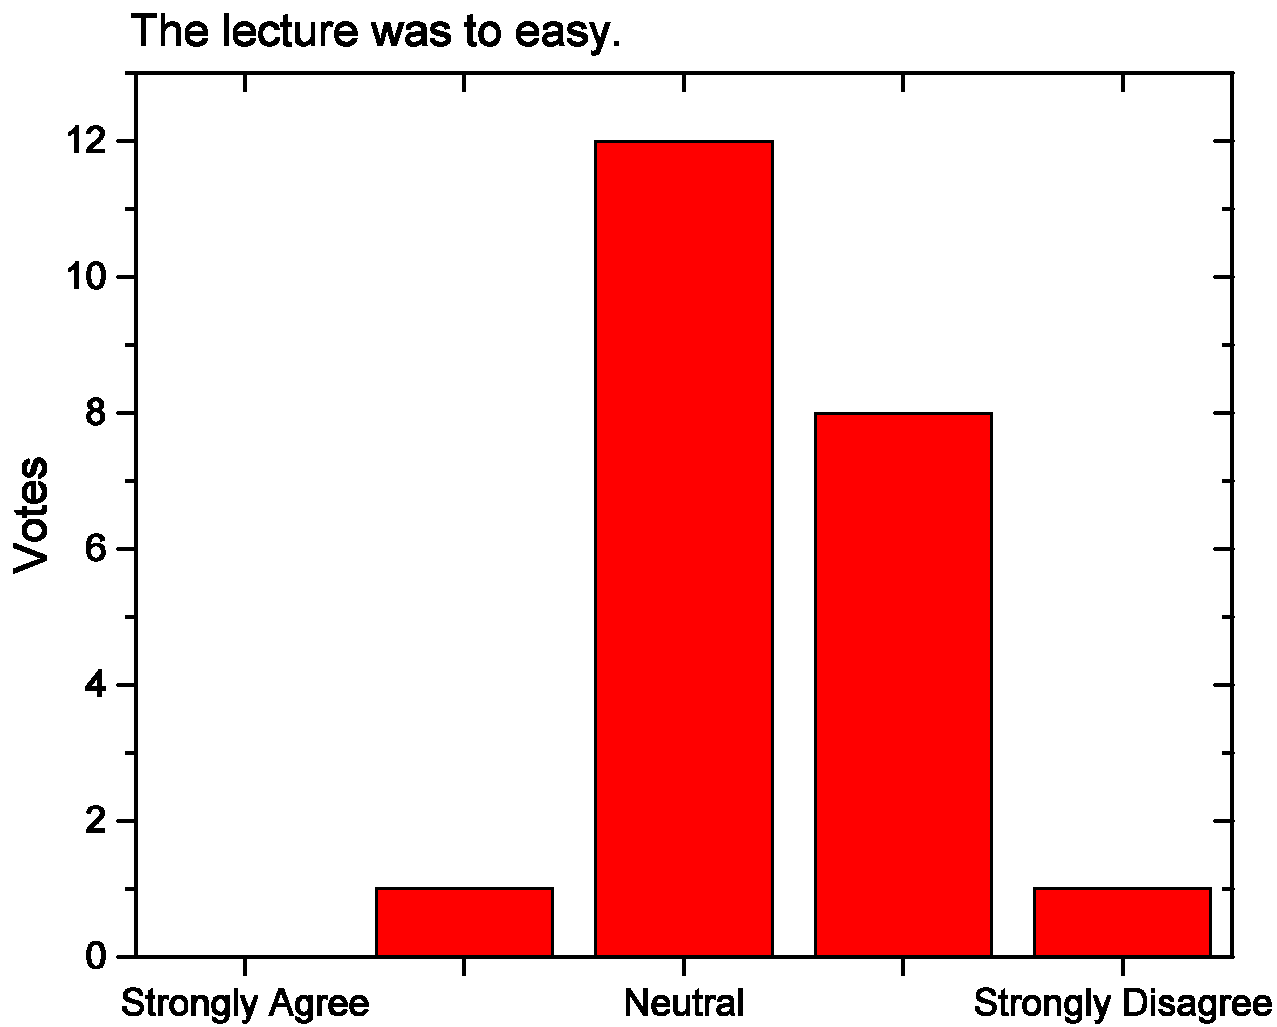
\includegraphics[height=50mm]{figures/n/Graph45.pdf}}
      {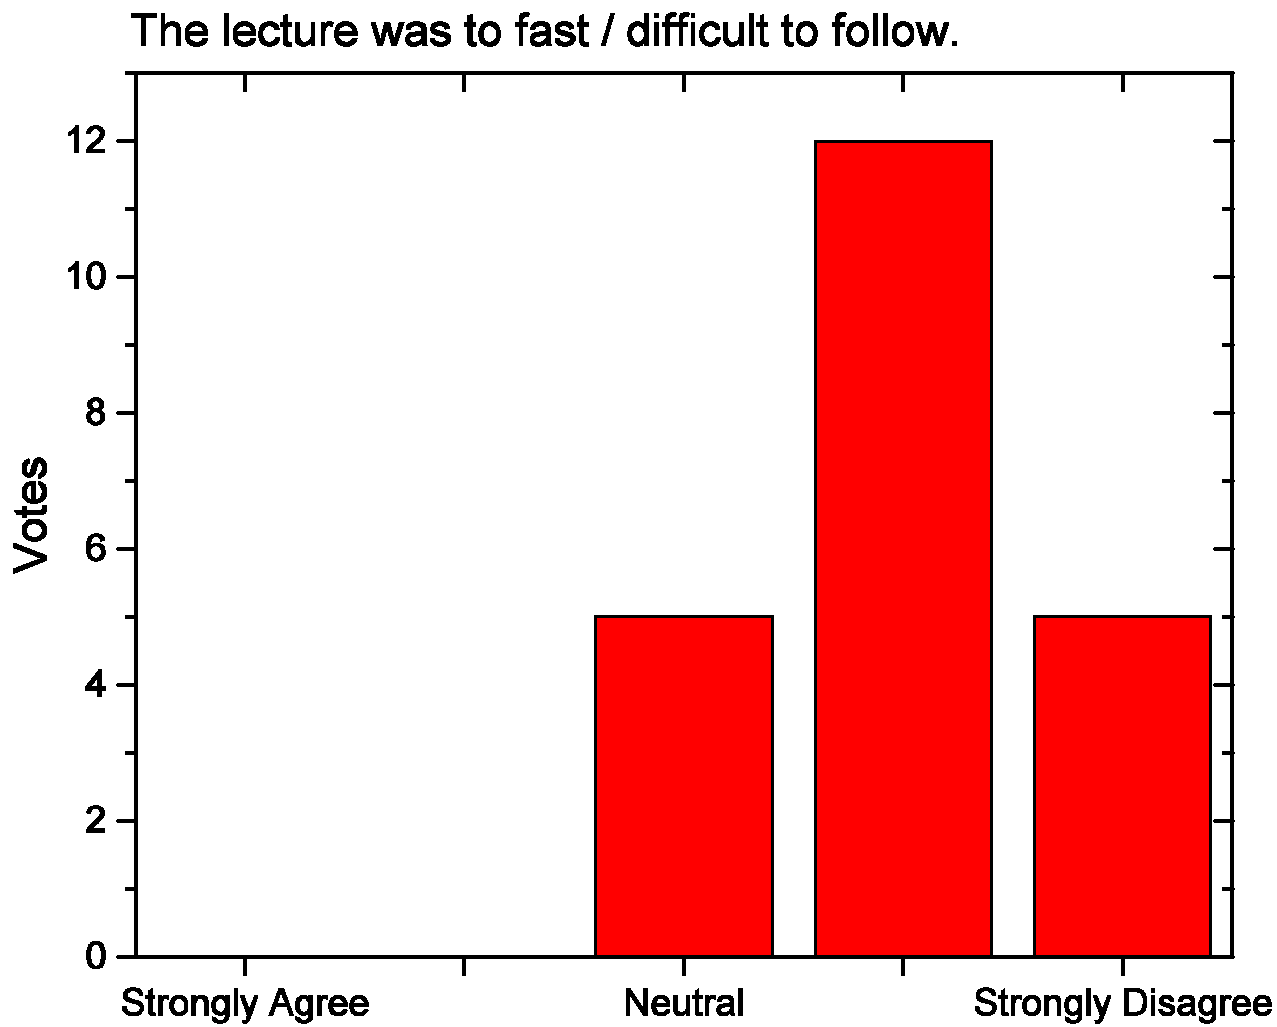
\includegraphics[height=50mm]{figures/n/Graph46.pdf}}
  \end{minipage}
\end{figure}

\begin{figure}[H]
  \begin{minipage}{.48\linewidth}
    \centering
      {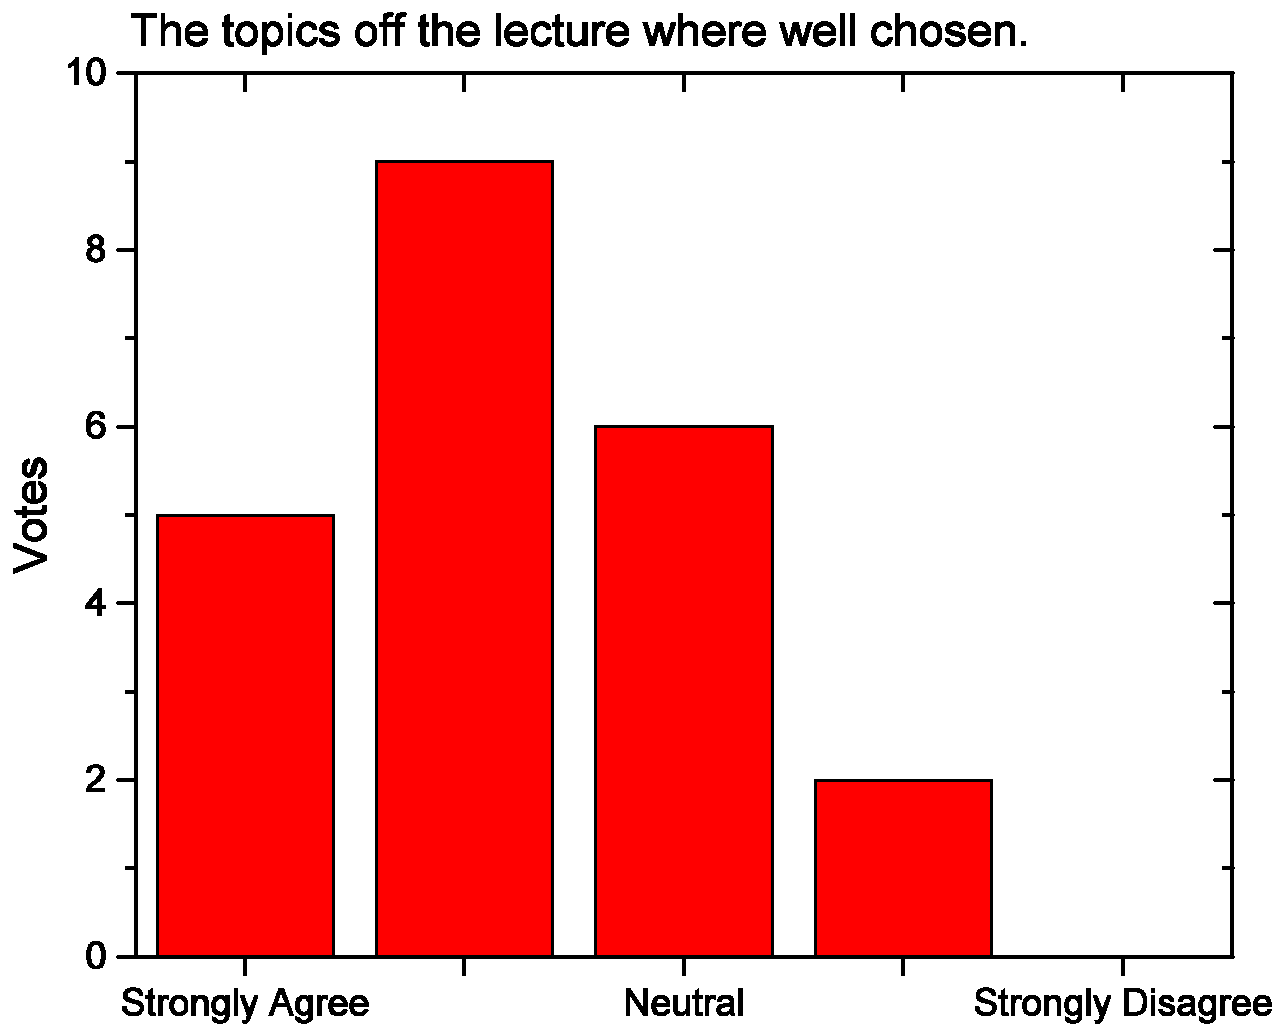
\includegraphics[height=50mm]{figures/n/Graph47.pdf}}
      {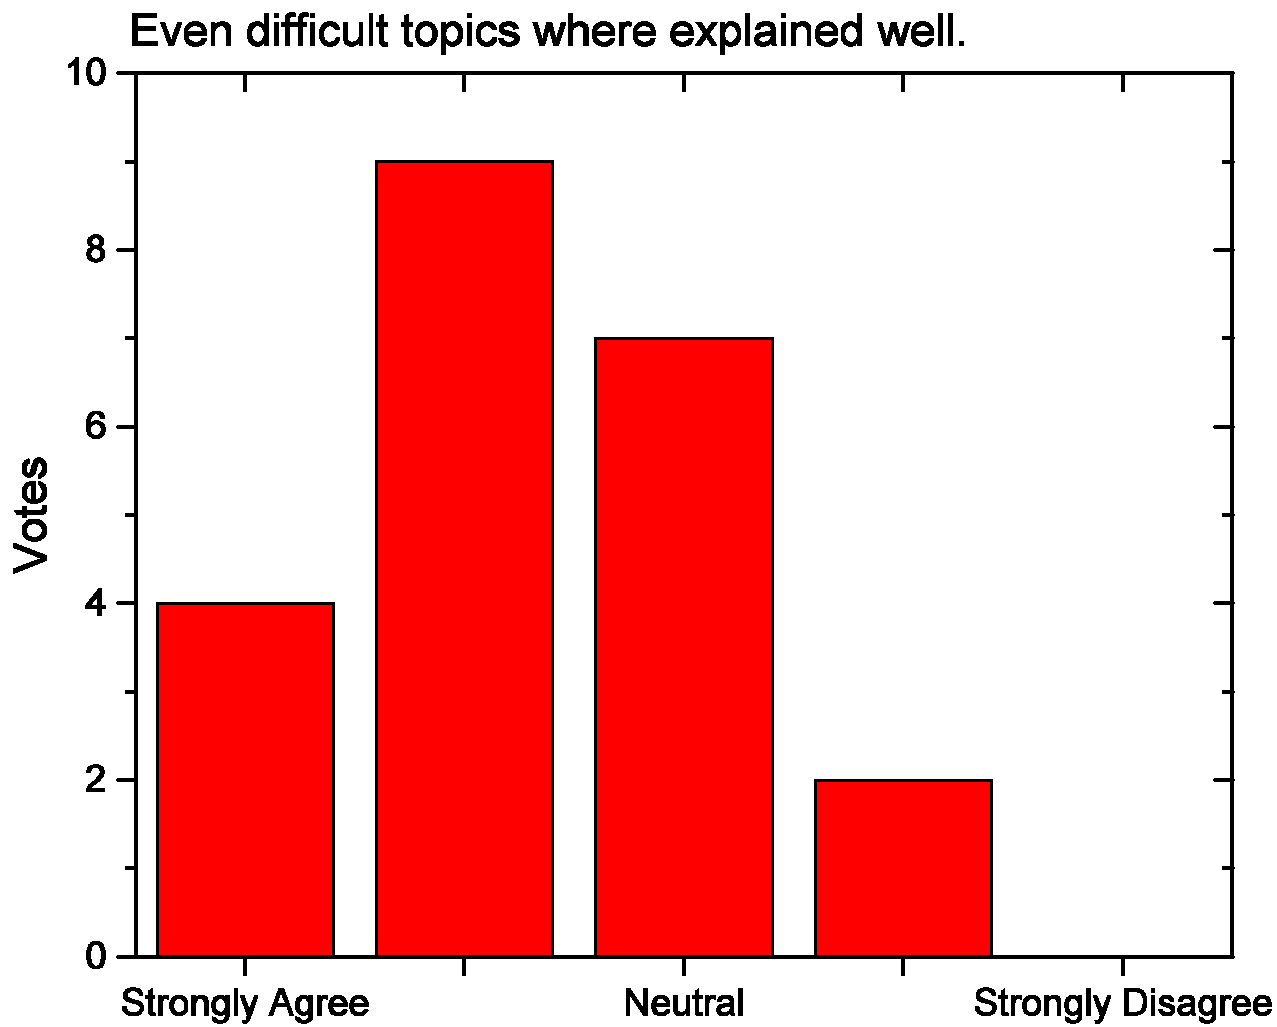
\includegraphics[height=50mm]{figures/n/Graph48.pdf}}
  \end{minipage}\quad
  \begin{minipage}{.48\linewidth}
    \centering
      {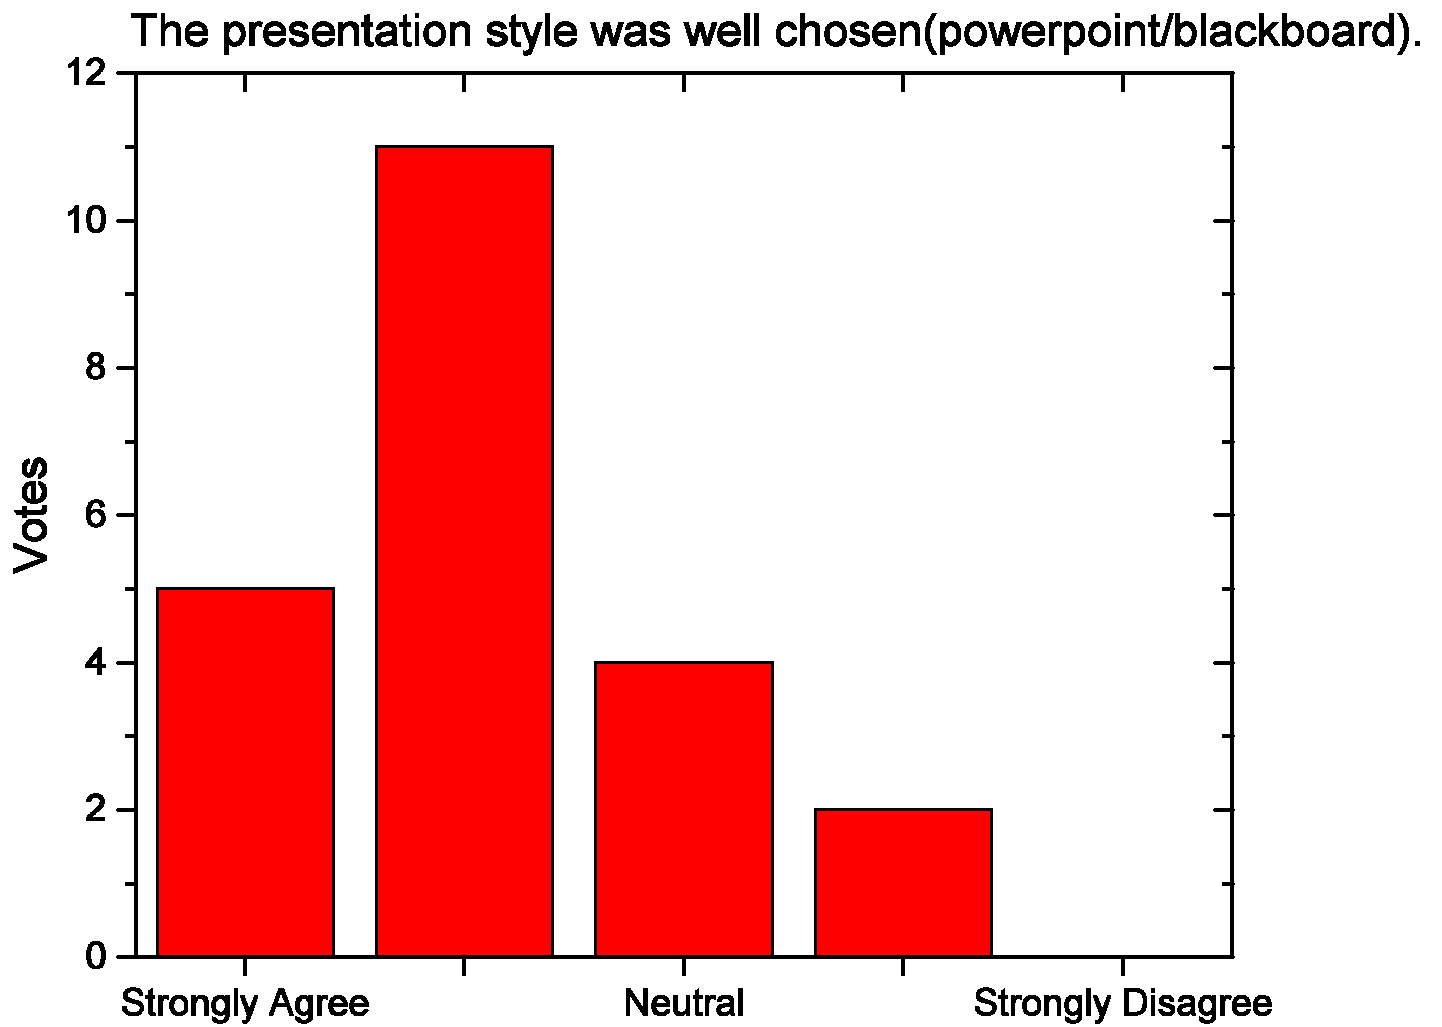
\includegraphics[height=50mm]{figures/n/Graph49.pdf}}
      {\includegraphics[height=50mm]{figures/n/Graph50.pdf}}
  \end{minipage}
\end{figure}
\subsubsection*{Comments}
\begin{itemize}
\item Overall good  and interesting but a bit too specialised.
\item Question were not answered very well.
\end{itemize}
\newpage


\subsubsection{Pascal Bohleber  --- The Physics of Glaciers }
\pdfbookmark{B2 Pascal Bohleber}{label:pb}
\begin{figure}[h!]
  \centering
  \begin{minipage}{.48\linewidth}
    \centering
      {\includegraphics[height=50mm]{figures/n/Graph51.pdf}}
      {\includegraphics[height=50mm]{figures/n/Graph52.pdf}}
      {\includegraphics[height=50mm]{figures/n/Graph53.pdf}}
  \end{minipage}\quad
  \begin{minipage}{.48\linewidth}
    \centering
      {\includegraphics[height=50mm]{figures/n/Graph54.pdf}}
      {\includegraphics[height=50mm]{figures/n/Graph55.pdf}}
      {\includegraphics[height=50mm]{figures/n/Graph56.pdf}}
  \end{minipage}
\end{figure}

\begin{figure}[H]
  \begin{minipage}{.48\linewidth}
    \centering
      {\includegraphics[height=50mm]{figures/n/Graph57.pdf}}
      {\includegraphics[height=50mm]{figures/n/Graph58.pdf}}
  \end{minipage}\quad
  \begin{minipage}{.48\linewidth}
    \centering
      {\includegraphics[height=50mm]{figures/n/Graph59.pdf}}
      {\includegraphics[height=50mm]{figures/n/Graph60.pdf}}
  \end{minipage}
\end{figure}
\subsubsection*{Comments}
-
\newpage

\subsubsection{Bj\"orn Malte Schäfer  --- General relativity in everyday life}
\pdfbookmark{B2 Bj\"orn Malte Schäfer}{label:bms}
\begin{figure}[h!]
  \centering
  \begin{minipage}{.48\linewidth}
    \centering
      {\includegraphics[height=50mm]{figures/n/Graph61.pdf}}
      {\includegraphics[height=50mm]{figures/n/Graph62.pdf}}
      {\includegraphics[height=50mm]{figures/n/Graph63.pdf}}
  \end{minipage}\quad
  \begin{minipage}{.48\linewidth}
    \centering
      {\includegraphics[height=50mm]{figures/n/Graph64.pdf}}
      {\includegraphics[height=50mm]{figures/n/Graph65.pdf}}
      {\includegraphics[height=50mm]{figures/n/Graph66.pdf}}
  \end{minipage}
\end{figure}

\begin{figure}[H]
  \begin{minipage}{.48\linewidth}
    \centering
      {\includegraphics[height=50mm]{figures/n/Graph67.pdf}}
      {\includegraphics[height=50mm]{figures/n/Graph68.pdf}}
  \end{minipage}\quad
  \begin{minipage}{.48\linewidth}
    \centering
      {\includegraphics[height=50mm]{figures/n/Graph69.pdf}}
      {\includegraphics[height=50mm]{figures/n/Graph70.pdf}}
  \end{minipage}
\end{figure}
\subsubsection*{Comments}
\begin{itemize}
\item Just amazing.
\end{itemize}
\newpage

\subsubsection{Morgan Fouesneau  --- Astrostatistics }
\pdfbookmark{B2 Morgan Fouesneau}{label:mf}
\begin{figure}[h!]
  \centering
  \begin{minipage}{.48\linewidth}
    \centering
      {\includegraphics[height=50mm]{figures/n/Graph71.pdf}}
      {\includegraphics[height=50mm]{figures/n/Graph72.pdf}}
      {\includegraphics[height=50mm]{figures/n/Graph73.pdf}}
  \end{minipage}\quad
  \begin{minipage}{.48\linewidth}
    \centering
      {\includegraphics[height=50mm]{figures/n/Graph74.pdf}}
      {\includegraphics[height=50mm]{figures/n/Graph75.pdf}}
      {\includegraphics[height=50mm]{figures/n/Graph76.pdf}}
  \end{minipage}
\end{figure}

\begin{figure}[H]
  \begin{minipage}{.48\linewidth}
    \centering
      {\includegraphics[height=50mm]{figures/n/Graph77.pdf}}
      {\includegraphics[height=50mm]{figures/n/Graph78.pdf}}
  \end{minipage}\quad
  \begin{minipage}{.48\linewidth}
    \centering
      {\includegraphics[height=50mm]{figures/n/Graph79.pdf}}
      {\includegraphics[height=50mm]{figures/n/Graph80.pdf}}
  \end{minipage}
\end{figure}
\subsubsection*{Comments}
-
\newpage


\subsubsection{Karlheinz Meier  --- Computers like brains - Physical model systems of neural circuits}
\pdfbookmark{B2 Karlheinz Meier}{label:khm}
\begin{figure}[h!]
  \centering
  \begin{minipage}{.48\linewidth}
    \centering
      {\includegraphics[height=50mm]{figures/n/Graph81.pdf}}
      {\includegraphics[height=50mm]{figures/n/Graph82.pdf}}
      {\includegraphics[height=50mm]{figures/n/Graph83.pdf}}
  \end{minipage}\quad
  \begin{minipage}{.48\linewidth}
    \centering
      {\includegraphics[height=50mm]{figures/n/Graph84.pdf}}
      {\includegraphics[height=50mm]{figures/n/Graph85.pdf}}
      {\includegraphics[height=50mm]{figures/n/Graph86.pdf}}
  \end{minipage}
\end{figure}

\begin{figure}[H]
  \begin{minipage}{.48\linewidth}
    \centering
      {\includegraphics[height=50mm]{figures/n/Graph87.pdf}}
      {\includegraphics[height=50mm]{figures/n/Graph88.pdf}}
  \end{minipage}\quad
  \begin{minipage}{.48\linewidth}
    \centering
      {\includegraphics[height=50mm]{figures/n/Graph89.pdf}}
      {\includegraphics[height=50mm]{figures/n/Graph90.pdf}}
  \end{minipage}
\end{figure}
\subsubsection*{Comments}
\begin{itemize}
\item Hands on demo was great unfortunately too little time.
\item Speaker had to jump a lot in his slides.
\end{itemize}
\newpage


\subsubsection{Craig Lawrie  --- Introduction to stringy physics }
\pdfbookmark{B2 Craig Lawrie}{label:cl}
\begin{figure}[h!]
  \centering
  \begin{minipage}{.48\linewidth}
    \centering
      {\includegraphics[height=50mm]{figures/n/Graph91.pdf}}
      {\includegraphics[height=50mm]{figures/n/Graph92.pdf}}
      {\includegraphics[height=50mm]{figures/n/Graph93.pdf}}
  \end{minipage}\quad
  \begin{minipage}{.48\linewidth}
    \centering
      {\includegraphics[height=50mm]{figures/n/Graph94.pdf}}
      {\includegraphics[height=50mm]{figures/n/Graph95.pdf}}
      {\includegraphics[height=50mm]{figures/n/Graph96.pdf}}
  \end{minipage}
\end{figure}

\begin{figure}[H]
  \begin{minipage}{.48\linewidth}
    \centering
      {\includegraphics[height=50mm]{figures/n/Graph97.pdf}}
      {\includegraphics[height=50mm]{figures/n/Graph98.pdf}}
  \end{minipage}\quad
  \begin{minipage}{.48\linewidth}
    \centering
      {\includegraphics[height=50mm]{figures/n/Graph99.pdf}}
      {\includegraphics[height=50mm]{figures/n/Graph100.pdf}}
  \end{minipage}
\end{figure}
\subsubsection*{Comments}
\begin{itemize}
\item First day was perfect second day a bit too fast
\end{itemize}
\newpage

\subsubsection{Niklaus Berger  --- As rare as it gets: Searching for charged lepton flavour violation }
\pdfbookmark{B2 Niklaus Berger}{label:nkb}
\begin{figure}[h!]
  \centering
  \begin{minipage}{.48\linewidth}
    \centering
      {\includegraphics[height=50mm]{figures/n/Graph101.pdf}}
      {\includegraphics[height=50mm]{figures/n/Graph102.pdf}}
      {\includegraphics[height=50mm]{figures/n/Graph103.pdf}}
  \end{minipage}\quad
  \begin{minipage}{.48\linewidth}
    \centering
      {\includegraphics[height=50mm]{figures/n/Graph104.pdf}}
      {\includegraphics[height=50mm]{figures/n/Graph105.pdf}}
      {\includegraphics[height=50mm]{figures/n/Graph106.pdf}}
  \end{minipage}
\end{figure}

\begin{figure}[H]
  \begin{minipage}{.48\linewidth}
    \centering
      {\includegraphics[height=50mm]{figures/n/Graph107.pdf}}
      {\includegraphics[height=50mm]{figures/n/Graph108.pdf}}
  \end{minipage}\quad
  \begin{minipage}{.48\linewidth}
    \centering
      {\includegraphics[height=50mm]{figures/n/Graph109.pdf}}
      {\includegraphics[height=50mm]{figures/n/Graph110.pdf}}
  \end{minipage}
\end{figure}
\subsubsection*{Comments}
-
\newpage